% \documentclass{article}


% % if you need to pass options to natbib, use, e.g.:
% %     \PassOptionsToPackage{numbers, compress}{natbib}
% % before loading neurips_2025

% \usepackage[numbers]{natbib}
% % ready for submission
% \usepackage{neurips_2026}
% \usepackage{enumitem}

% to compile a preprint version, e.g., for submission to arXiv, add add the
% [preprint] option:
%     \usepackage[preprint]{neurips_2025}


% to compile a camera-ready version, add the [final] option, e.g.:
%     \usepackage[final]{neurips_2025}


% to avoid loading the natbib package, add option nonatbib:
%    \usepackage[nonatbib]{neurips_2025}


% \usepackage[utf8]{inputenc} % allow utf-8 input
% \usepackage[T1]{fontenc}    % use 8-bit T1 fonts
% %\usepackage{hyperref}       % hyperlinks
% \usepackage{url}            % simple URL typesetting
% \usepackage{booktabs}       % professional-quality tables
% \usepackage{amsfonts}       % blackboard math symbols
% \usepackage{nicefrac}       % compact symbols for 1/2, etc.
% \usepackage{microtype}      % microtypography
% \usepackage{xcolor}         % colors
% \usepackage{graphicx}
% \usepackage{amsmath,amssymb}
% \usepackage{tikz}
% \usepackage[
%   dvipsnames,   % ≈ 68 extra names
%   svgnames,     % ≈ 151 SVG names (includes LightSkyBlue, SkyBlue, …)
%   x11names      % ≈ 140 X11 names (PowderBlue, LightBlue, …)
% ]{xcolor}

% \usepackage{subcaption}
% \usepackage{algorithm}
% \usepackage{algorithmic}

% \usepackage{comment}
% \usepackage{import}
% %\subimport{Neurips2025}{packages}
% %\subimport{Neurips2025}{macros}

% \usepackage{placeins}

% \usepackage{import, hyperref}
% % To have short pointers for sections and subsections. Oren Freifeld
% \renewcommand{\sectionautorefname}{\S} 
% \renewcommand{\subsectionautorefname}{\S} 
% \renewcommand{\subsubsectionautorefname}{\S} 
% \renewcommand{\equationautorefname}{Eq.}
% %\renewcommand{\figureautorefname}{Fig.}
% % \Autoref is for the beginning of the sentence
% \let\orgautoref\autoref
% \newcommand{\Autoref}[1]{%
% \begingroup%
% \renewcommand{\equationautorefname}{Equation}%
% \renewcommand{\figureautorefname}{Figure}%
% \autoref{#1}%
% \endgroup%
% }



\begin{center}
{\LARGE \textbf{SemGeo-Gen: Unsupervised Generation of Approximate Cross-Instance Semantic-Geometric Correspondences}}\\[4pt]
{\large ------------}\\[4pt]
{\LARGE \textbf{Supplementary Material}}
\end{center}

\vspace{1em}


% The \author macro works with any number of authors. There are two commands
% used to separate the names and addresses of multiple authors: \And and \AND.
%
% Using \And between authors leaves it to LaTeX to determine where to break the
% lines. Using \AND forces a line break at that point. So, if LaTeX puts 3 of 4
% authors names on the first line, and the last on the second line, try using
% \AND instead of \And before the third author name.


\author{%
  David S.~Hippocampus\thanks{Use footnote for providing further information
    about author (webpage, alternative address)---\emph{not} for acknowledging
    funding agencies.} \\
  Department of Computer Science\\
  Cranberry-Lemon University\\
  Pittsburgh, PA 15213 \\
  \texttt{hippo@cs.cranberry-lemon.edu} \\
  % examples of more authors
  % \And
  % Coauthor \\
  % Affiliation \\
  % Address \\
  % \texttt{email} \\
  % \AND
  % Coauthor \\
  % Affiliation \\
  % Address \\
  % \texttt{email} \\
  % \And
  % Coauthor \\
  % Affiliation \\
  % Address \\
  % \texttt{email} \\
  % \And
  % Coauthor \\
  % Affiliation \\
  % Address \\
  % \texttt{email} \\
}




In this supplementary material, we provide additional qualitative results, extended ablations, and detailed per-label analysis to complement the main paper.


\section*{Contents}
\begin{enumerate}[]
    \item \autoref{sup:qualitative} - Qualitative Results on SPair-71k and KeypointNet.
    \item \autoref{sup:supp_spair} - Additional Quantitative Results on SPair-71k.
    \item \autoref{sup:ablation_study} - Extended Ablation Study.
    \item \autoref{sup:supp_semantic_analy} - Qualitative Analysis of DINOv2 Based Semantic Filtering.
    \item \autoref{Sup:per_label} - Detailed PCK Results by Semantic Label and KeypointNet Category.
\end{enumerate}
\clearpage

\section{Qualitative Results}
\label{sup:qualitative}

\subsection{SPair-71k Transfer Results}

We provide qualitative SPair-71k \cite{min2019spair71k} examples comparing models trained only on real SPair-71k annotations with the same models pretrained on our generated synthetic correspondences and then fine-tuned on SPair-71k. We show results for both MARCO \cite{cuttano2026marco} (see \autoref{fig:qual_marco}) and GeoAware-SC \cite{zhang2024tellingLeftFromRight} (see \autoref{fig:qual_geoaware}).


\begin{figure*}[h]
\centering
\setlength{\tabcolsep}{3pt}
\begin{tabular}{cc}
\textbf{MARCO \cite{cuttano2026marco} Real-only} & \textbf{MARCO \cite{cuttano2026marco} Ours P.T.$\rightarrow$Real} \\
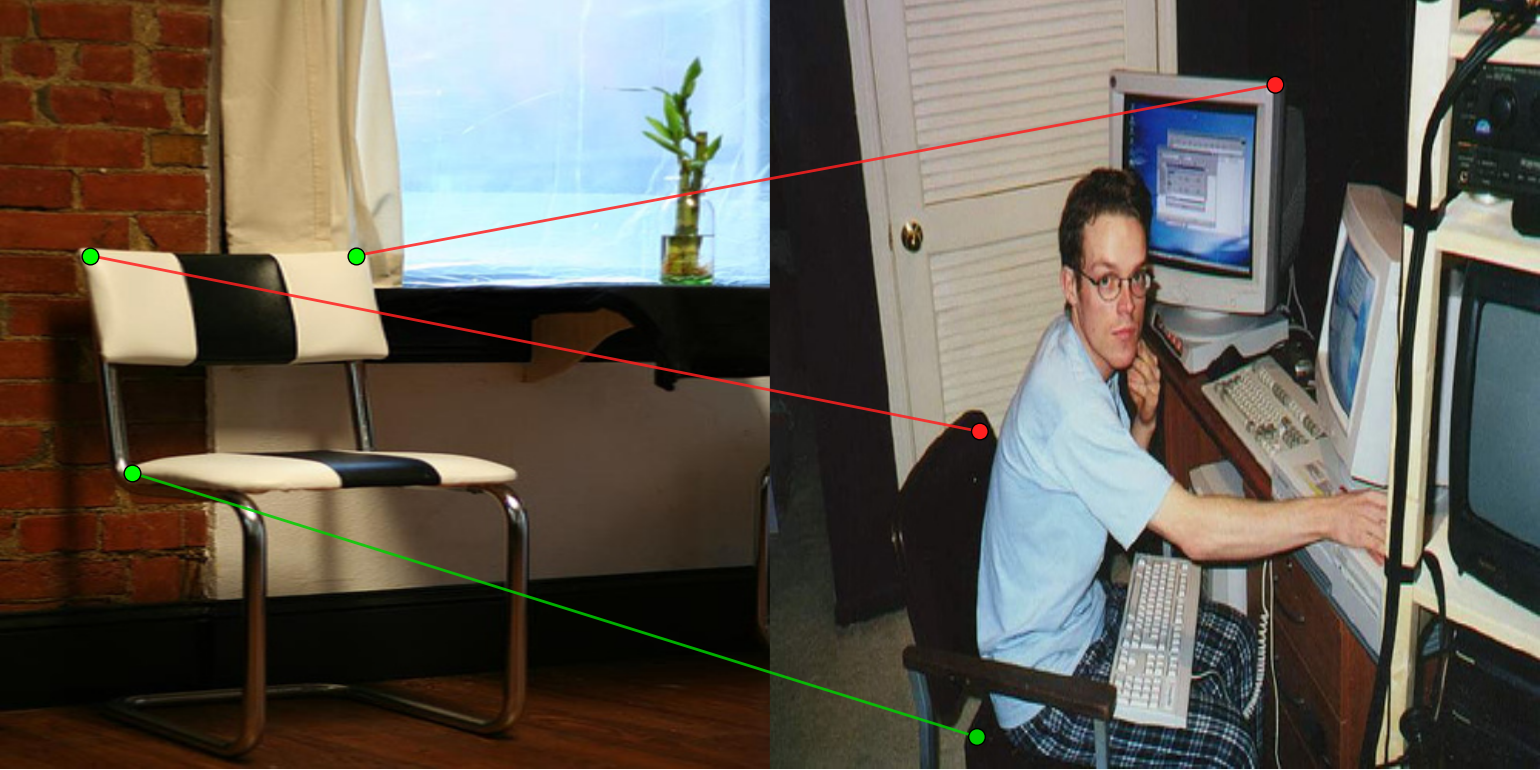
\includegraphics[width=0.48\textwidth]{figures/qualitative/marco/match_real_chair.png} &
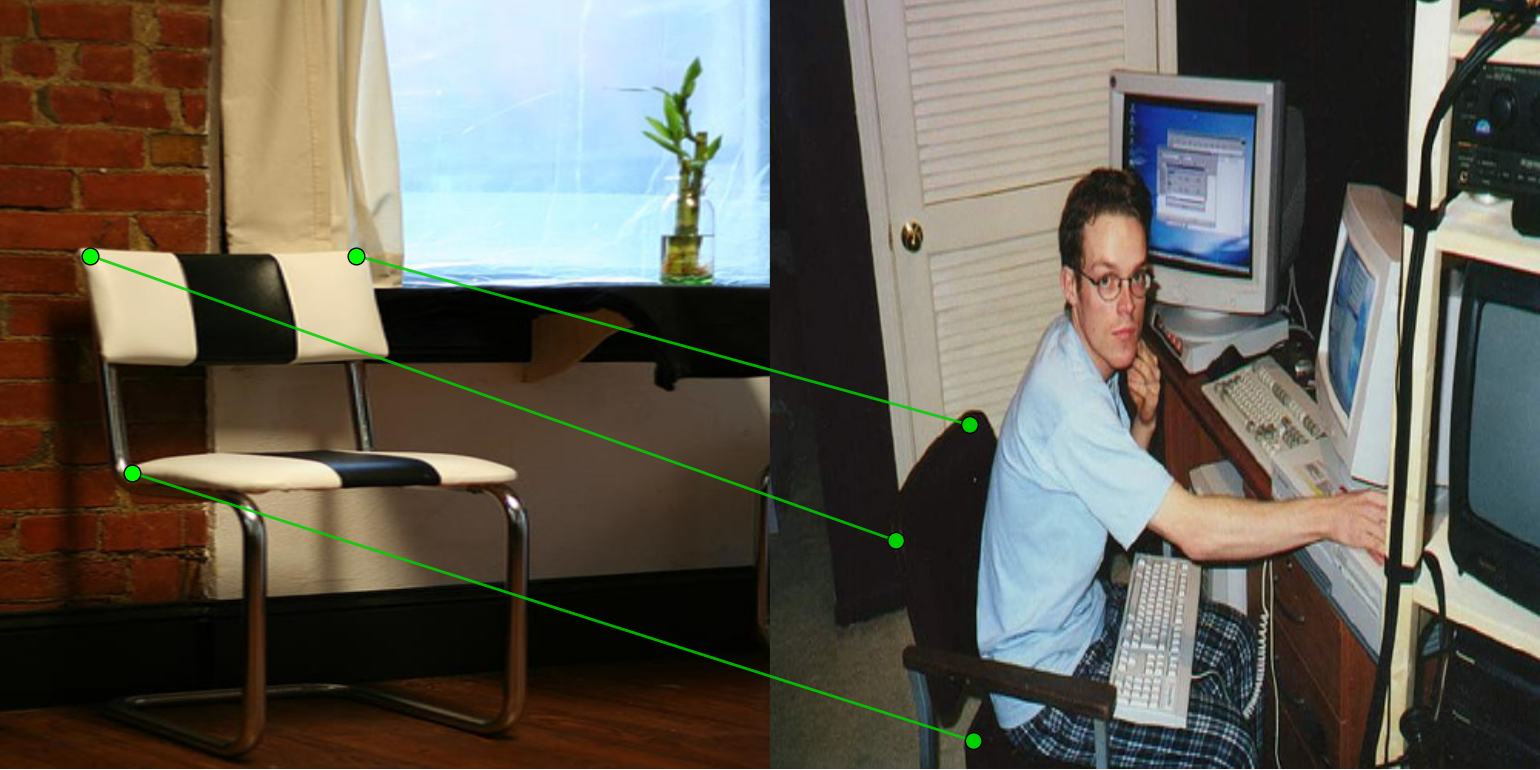
\includegraphics[width=0.48\textwidth]{figures/qualitative/marco/match_ours_chair.png} \\
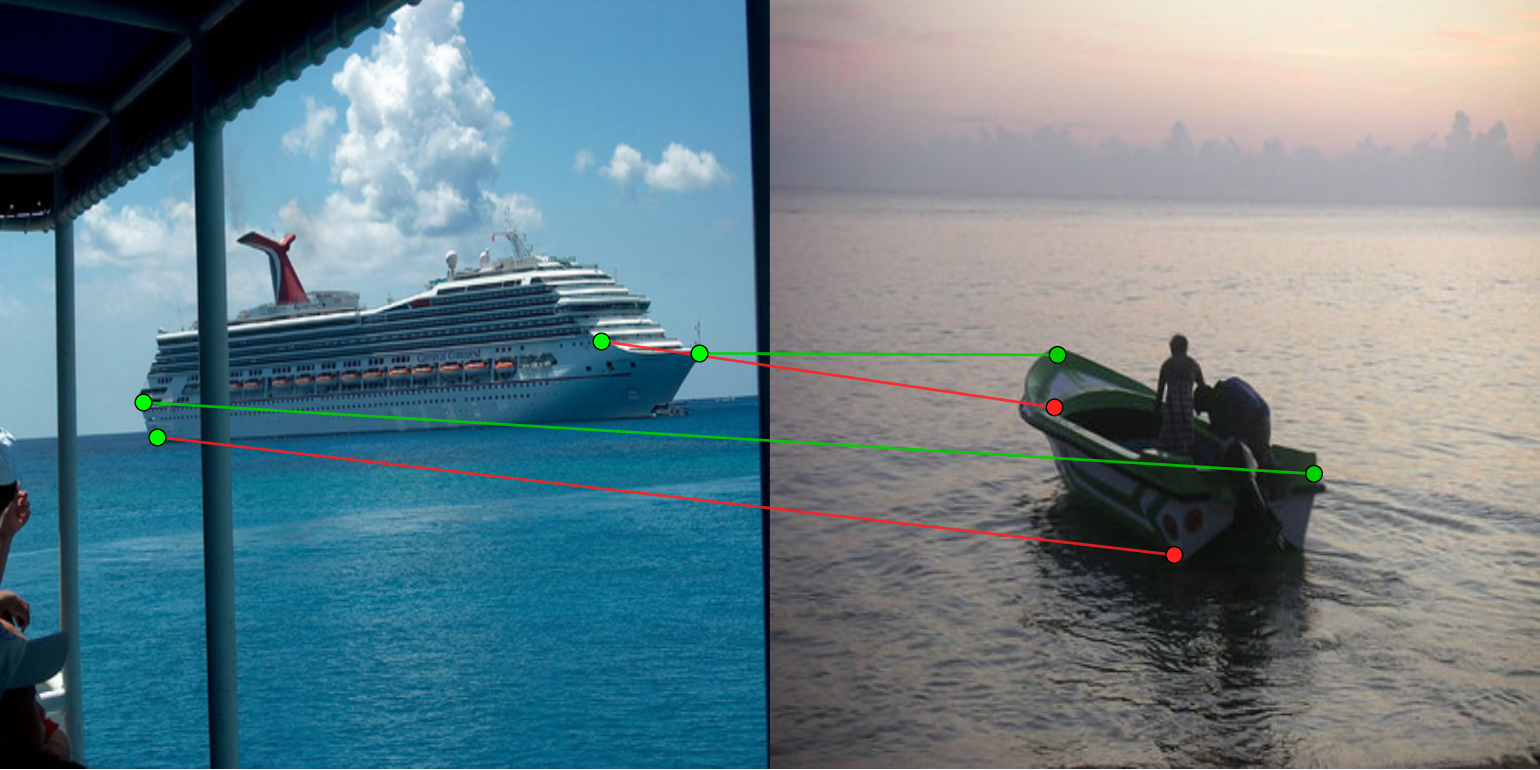
\includegraphics[width=0.48\textwidth]{figures/qualitative/marco/match_real_boat.png} &
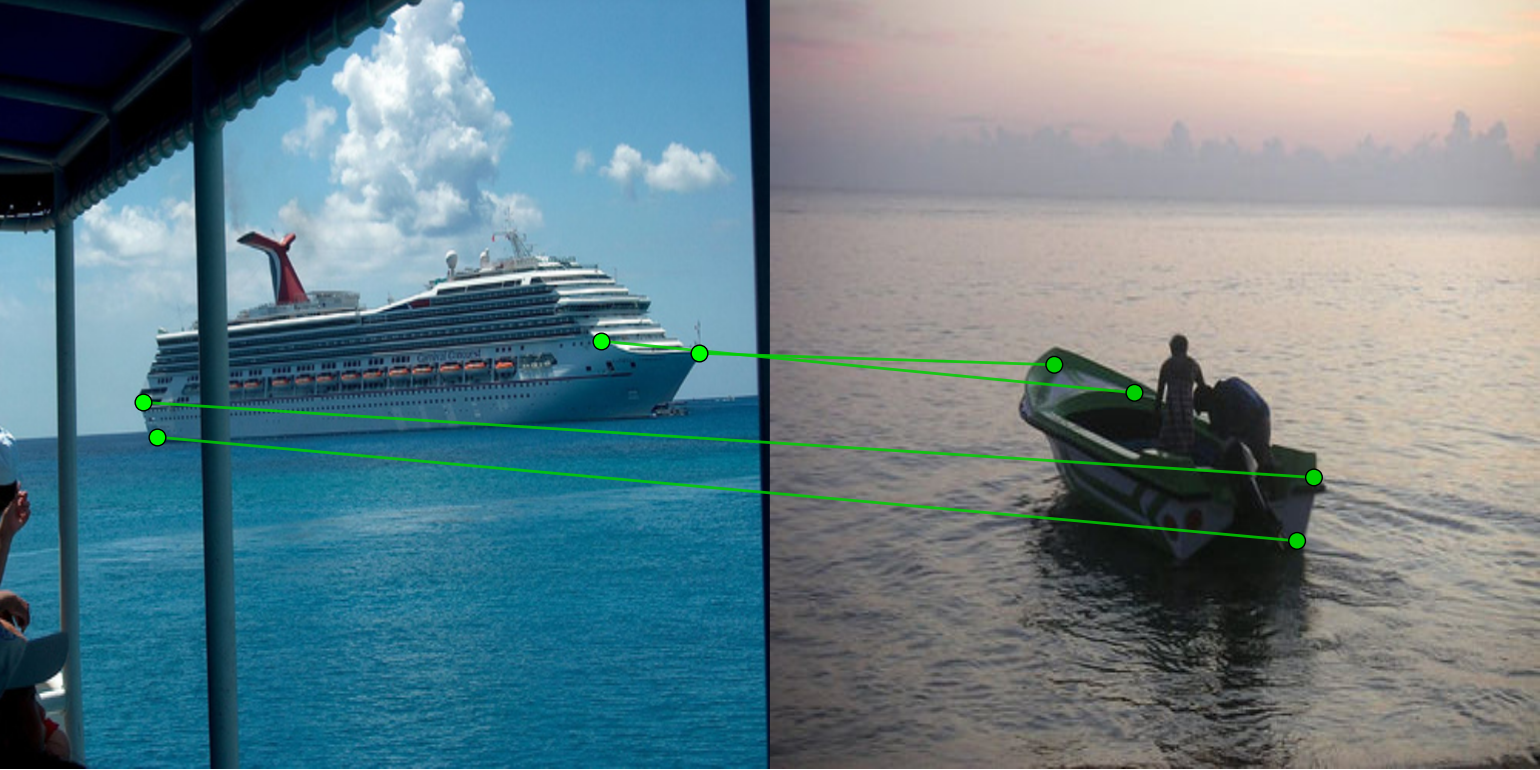
\includegraphics[width=0.48\textwidth]{figures/qualitative/marco/match_ours_boat.png} \\
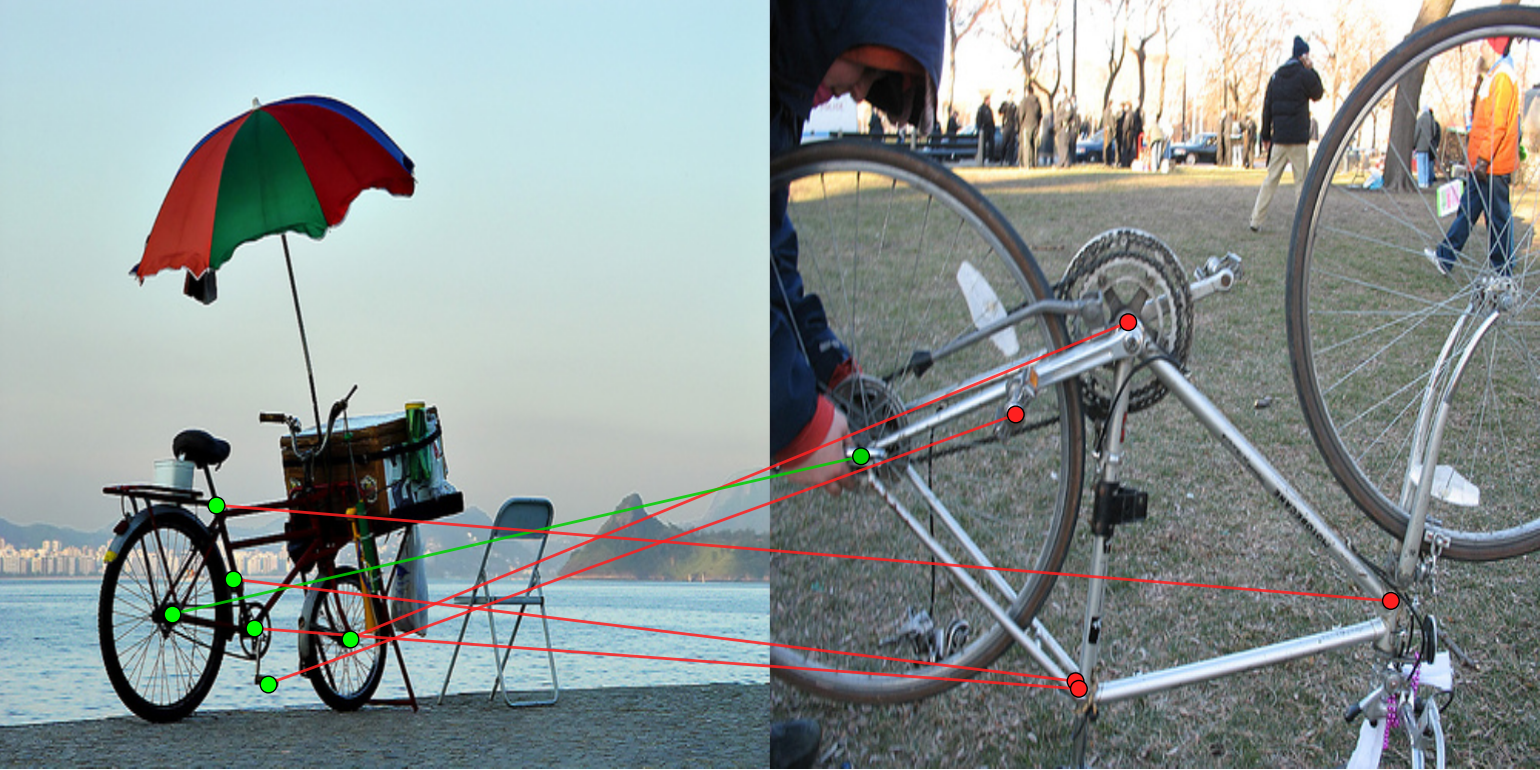
\includegraphics[width=0.48\textwidth]{figures/qualitative/marco/match_real_bicycle.png} &
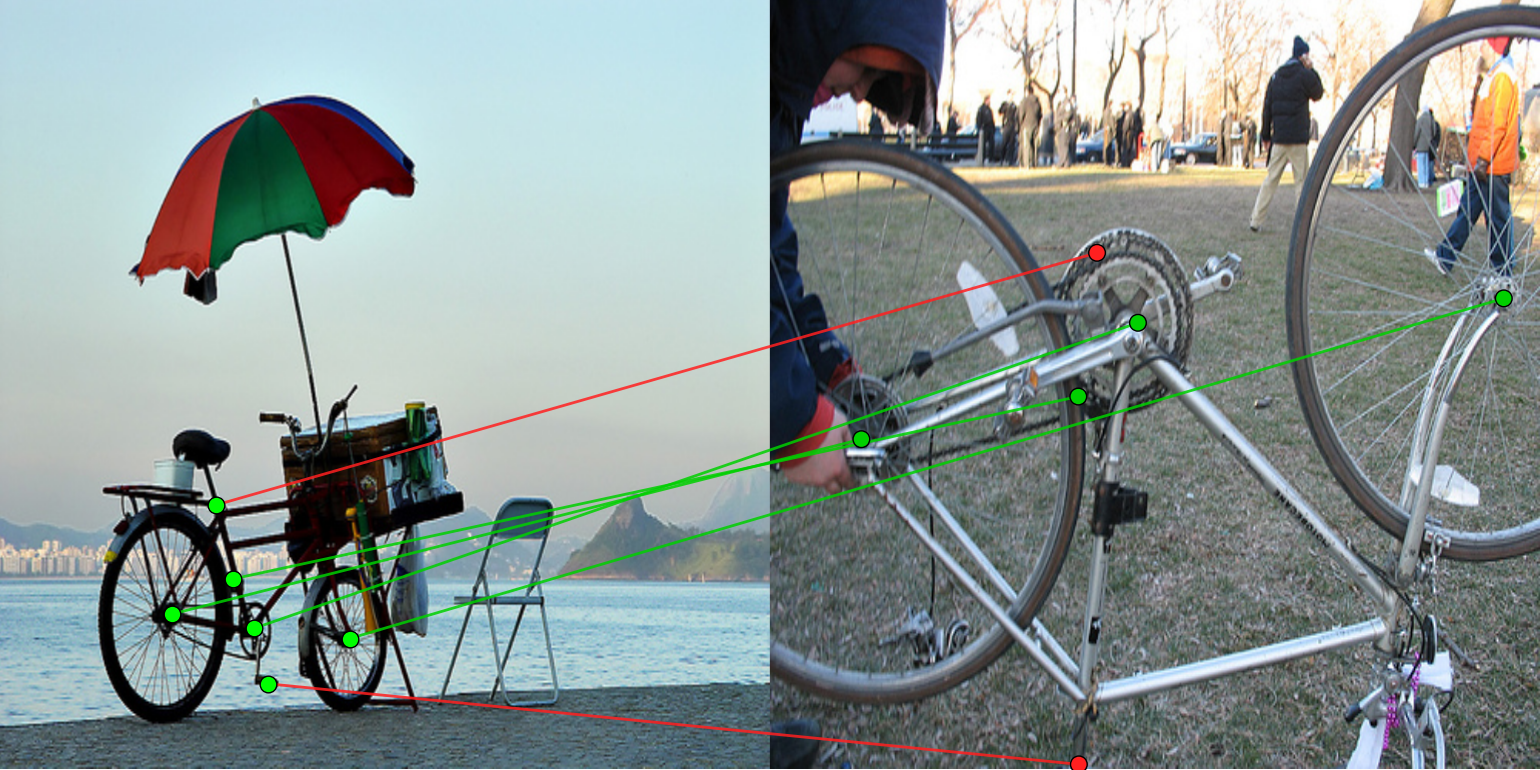
\includegraphics[width=0.48\textwidth]{figures/qualitative/marco/match_ours_bicycle.png} \\
\end{tabular}
\caption{\textbf{Qualitative SPair-71k \cite{min2019spair71k} results for MARCO \cite{cuttano2026marco}.}
Each image shows a source--target pair with predicted correspondences. We compare MARCO trained on SPair-71k against MARCO pretrained on our generated correspondences and then fine-tuned on SPair-71k.}
\label{fig:qual_marco}
\end{figure*}


\begin{figure*}[t]
\centering
\setlength{\tabcolsep}{3pt}
\begin{tabular}{cc}
\textbf{GeoAware-SC Real-only} & \textbf{GeoAware-SC Ours P.T.$\rightarrow$Real} \\
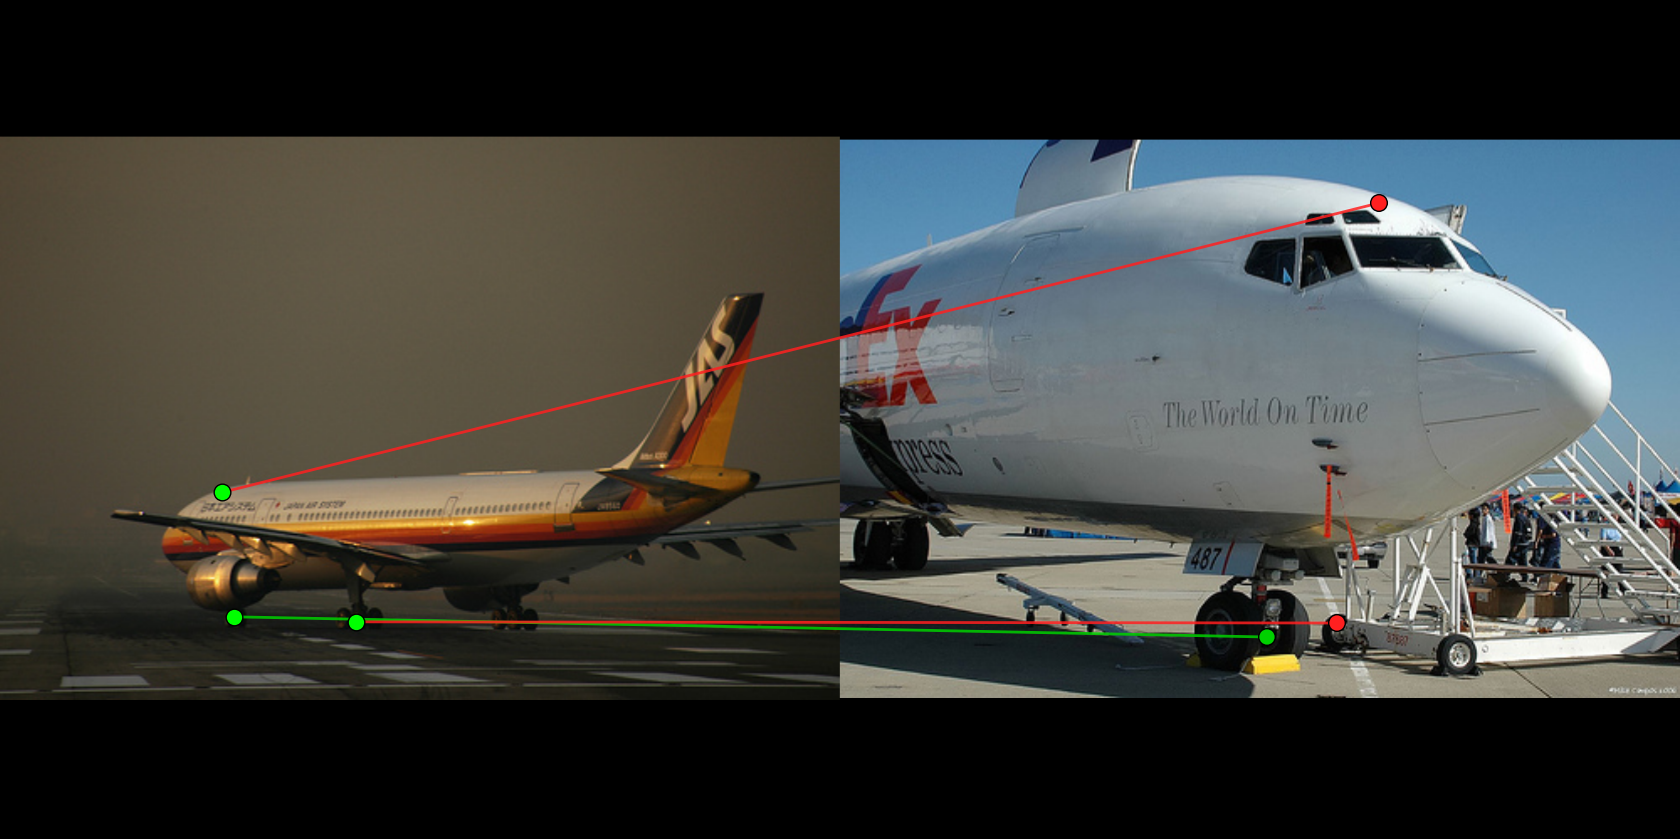
\includegraphics[width=0.48\textwidth]{figures/qualitative/geoaware/match_real_airplane.png} &
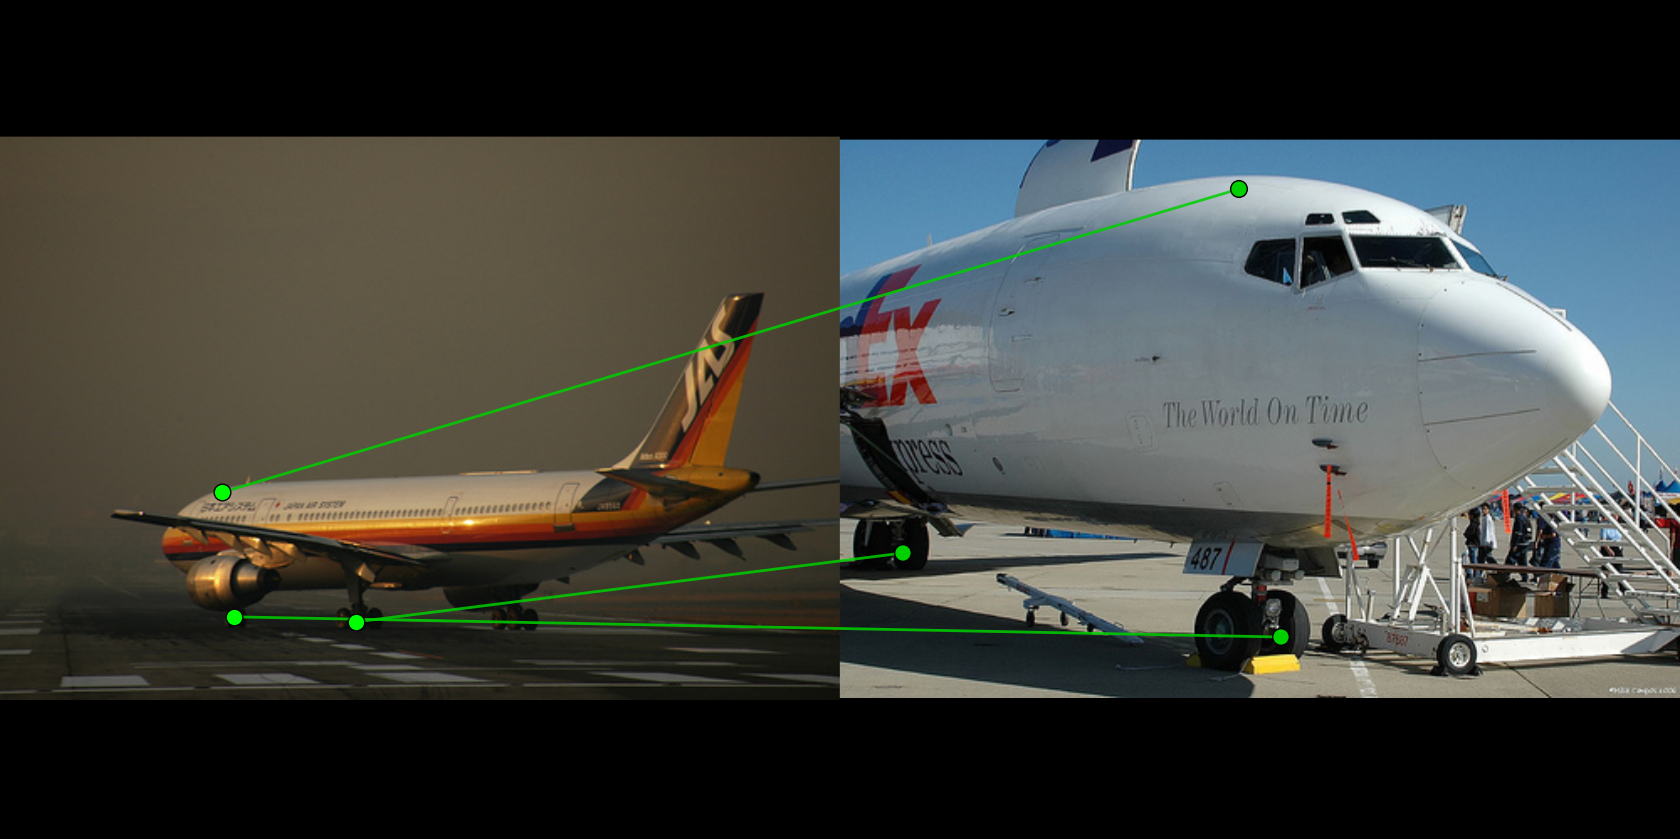
\includegraphics[width=0.48\textwidth]{figures/qualitative/geoaware/match_ours_airplane.png} \\
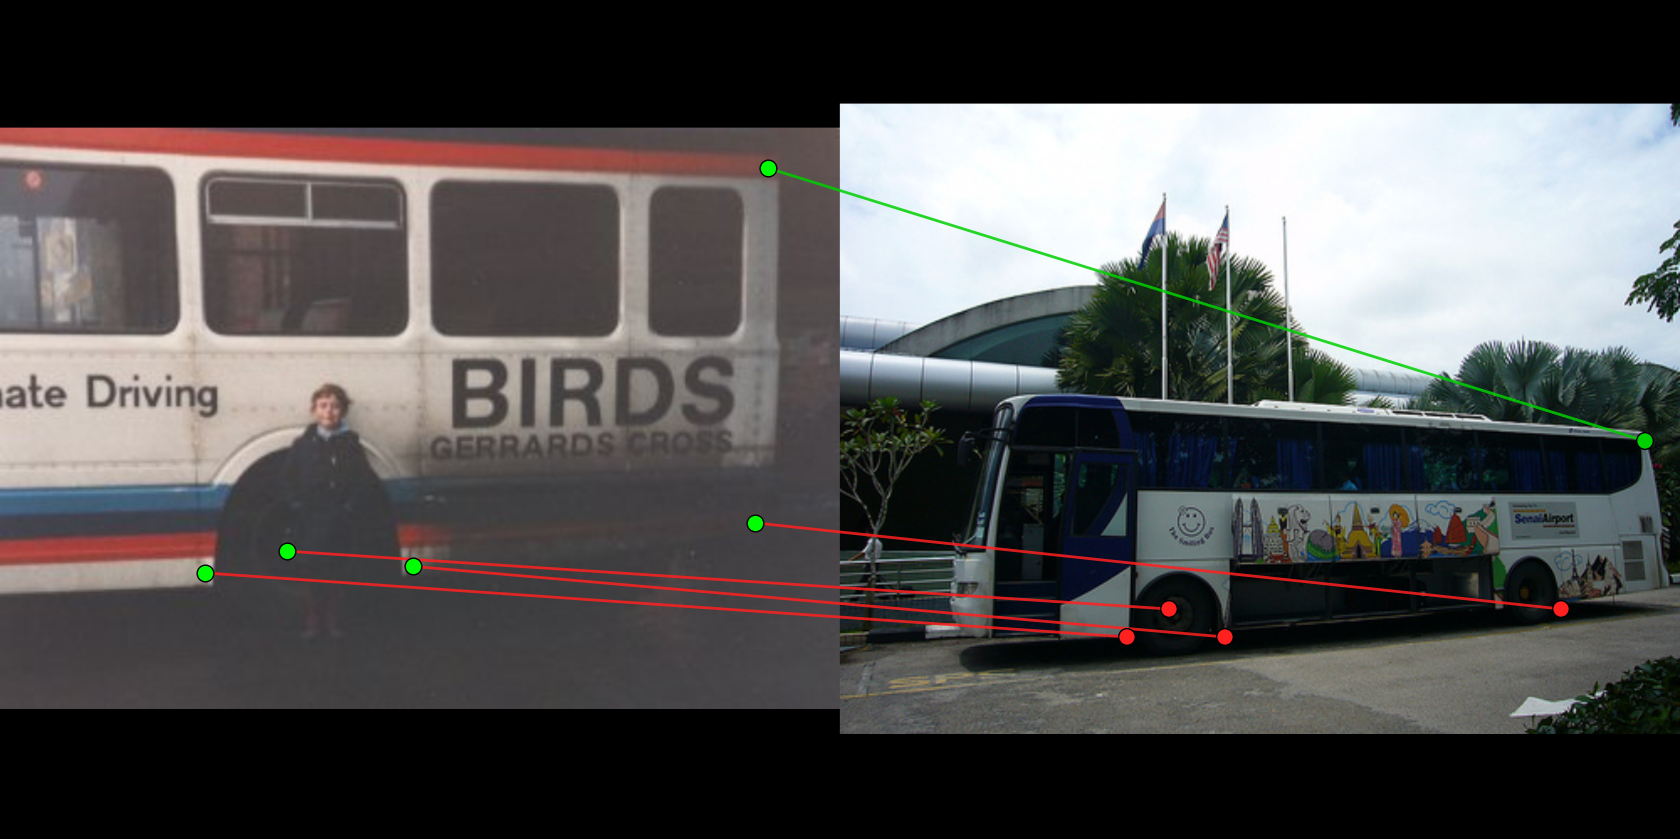
\includegraphics[width=0.48\textwidth]{figures/qualitative/geoaware/match_real_bus.png} &
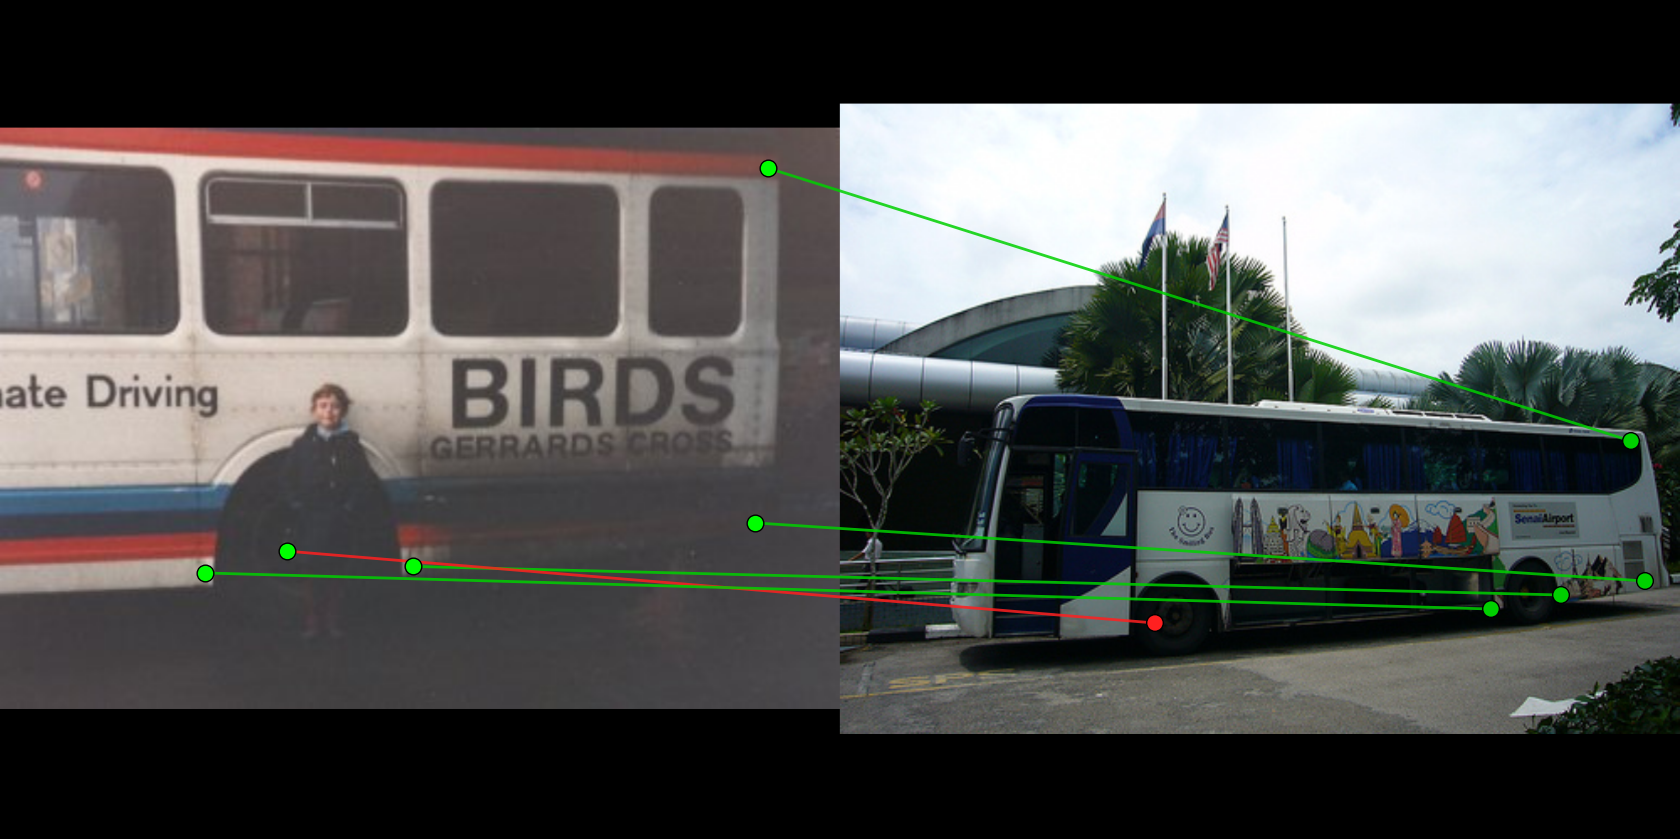
\includegraphics[width=0.48\textwidth]{figures/qualitative/geoaware/match_ours_bus.png} \\
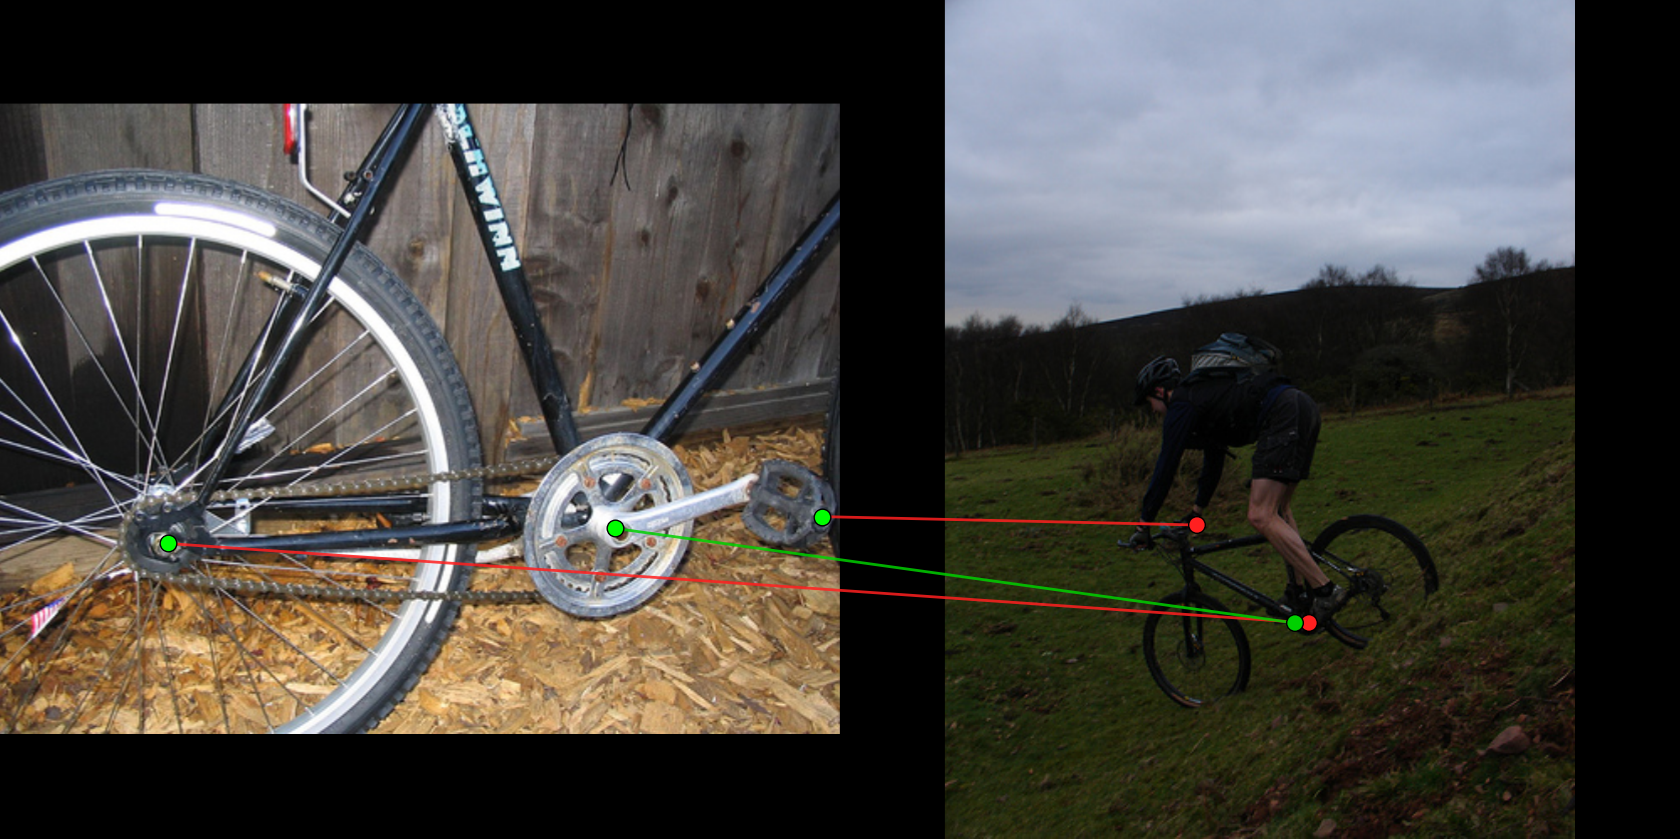
\includegraphics[width=0.48\textwidth]{figures/qualitative/geoaware/match_real_bike.png} &
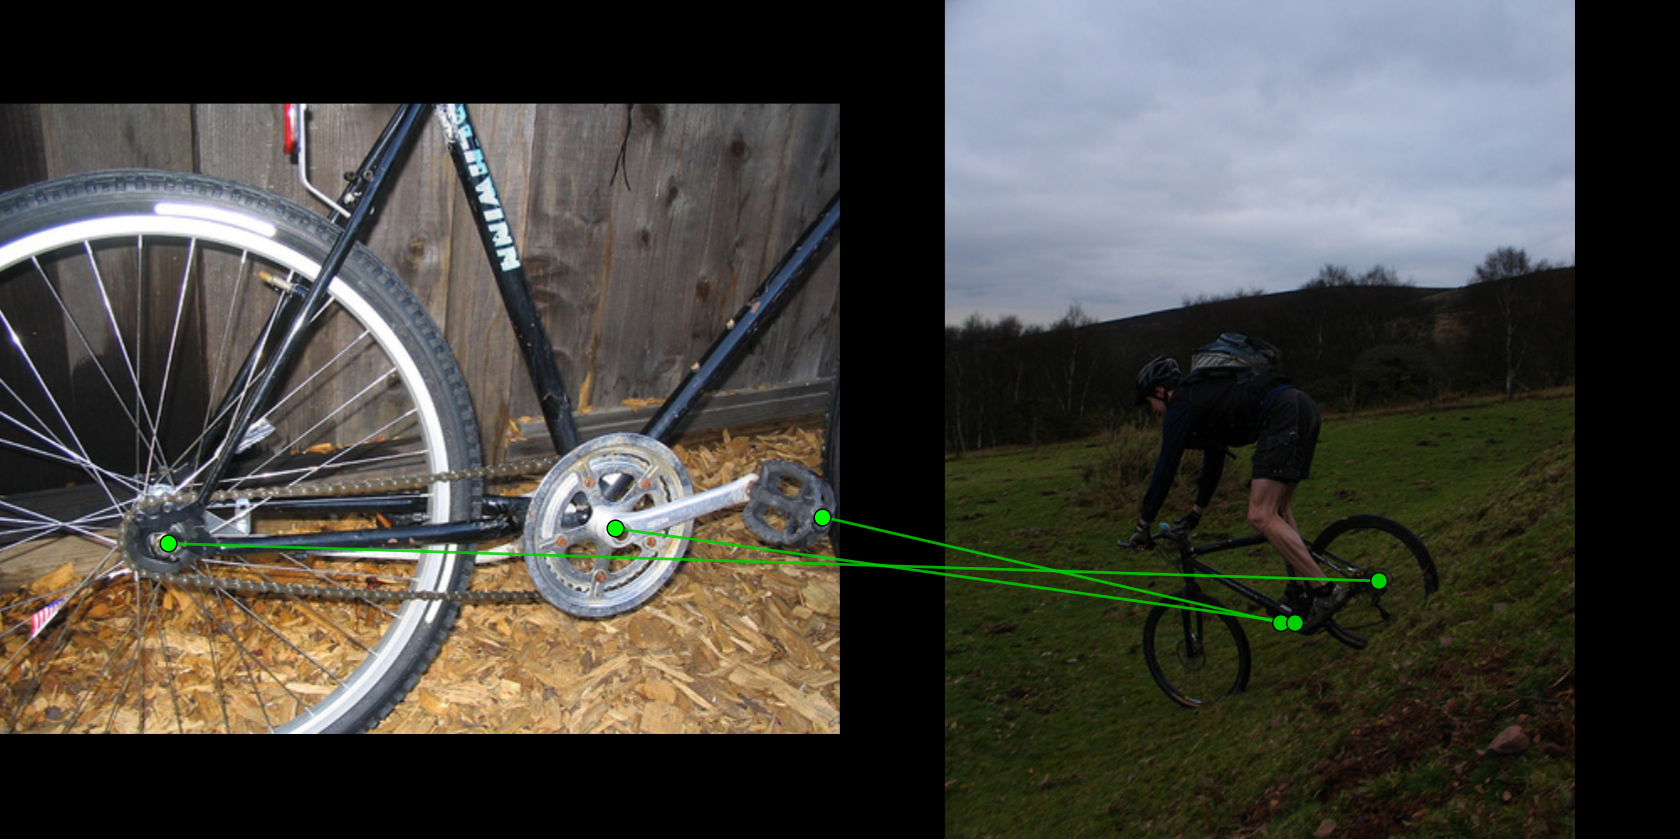
\includegraphics[width=0.48\textwidth]{figures/qualitative/geoaware/match_ours_bike.png} \\
\end{tabular}
\caption{\textbf{Qualitative SPair-71k \cite{min2019spair71k} results for GeoAware-SC \cite{zhang2024tellingLeftFromRight}.}
Each image shows a source--target pair with predicted correspondences. We compare GeoAware-SC trained on SPair-71k against GeoAware-SC pretrained on our generated correspondences and then fine-tuned on SPair-71k.}
\label{fig:qual_geoaware}
\end{figure*}

\clearpage
\subsection{Correspondence Examples on New Categories}

We additionally show (\autoref{fig:new_categories_examples}) qualitative correspondence examples on rigid categories beyond those covered by existing correspondence benchmarks such as SPair-71k \cite{min2019spair71k}, KeypointNet \cite{you2020}, and AP-10K \cite{yu2021AP10k}. These examples demonstrate the ability of our method to establish approximate semantic-geometric correspondences on diverse categories from Objaverse-OA \cite{orient_anything}.

\begin{figure*}[h]
\centering
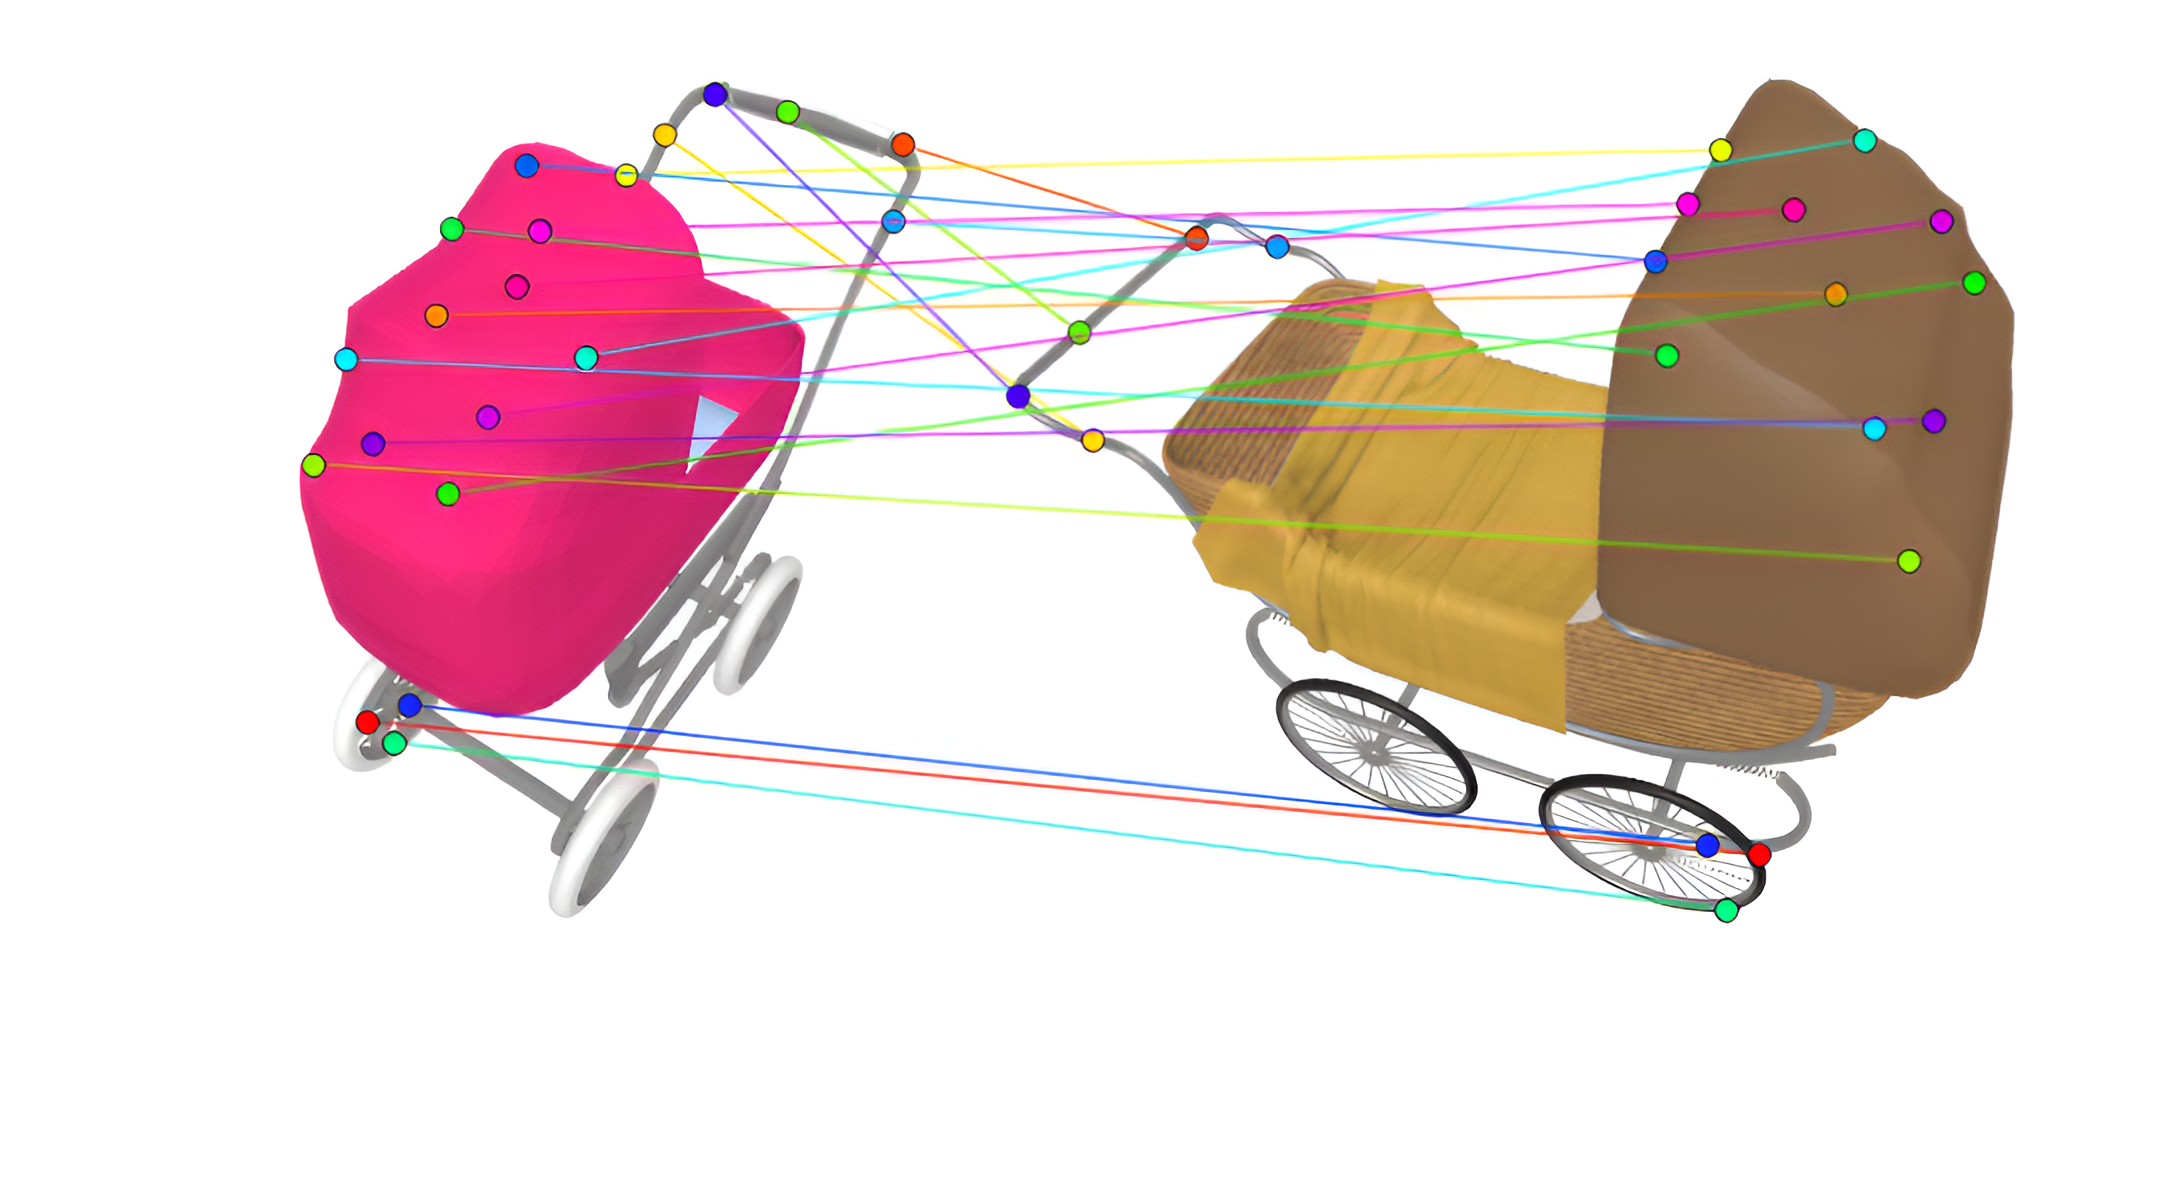
\includegraphics[width=0.92\linewidth,height=0.22\textheight,keepaspectratio,trim={100 150 100 40},clip]{figures/matching_examples/baby_buggy_highres.png}\vspace{1mm}

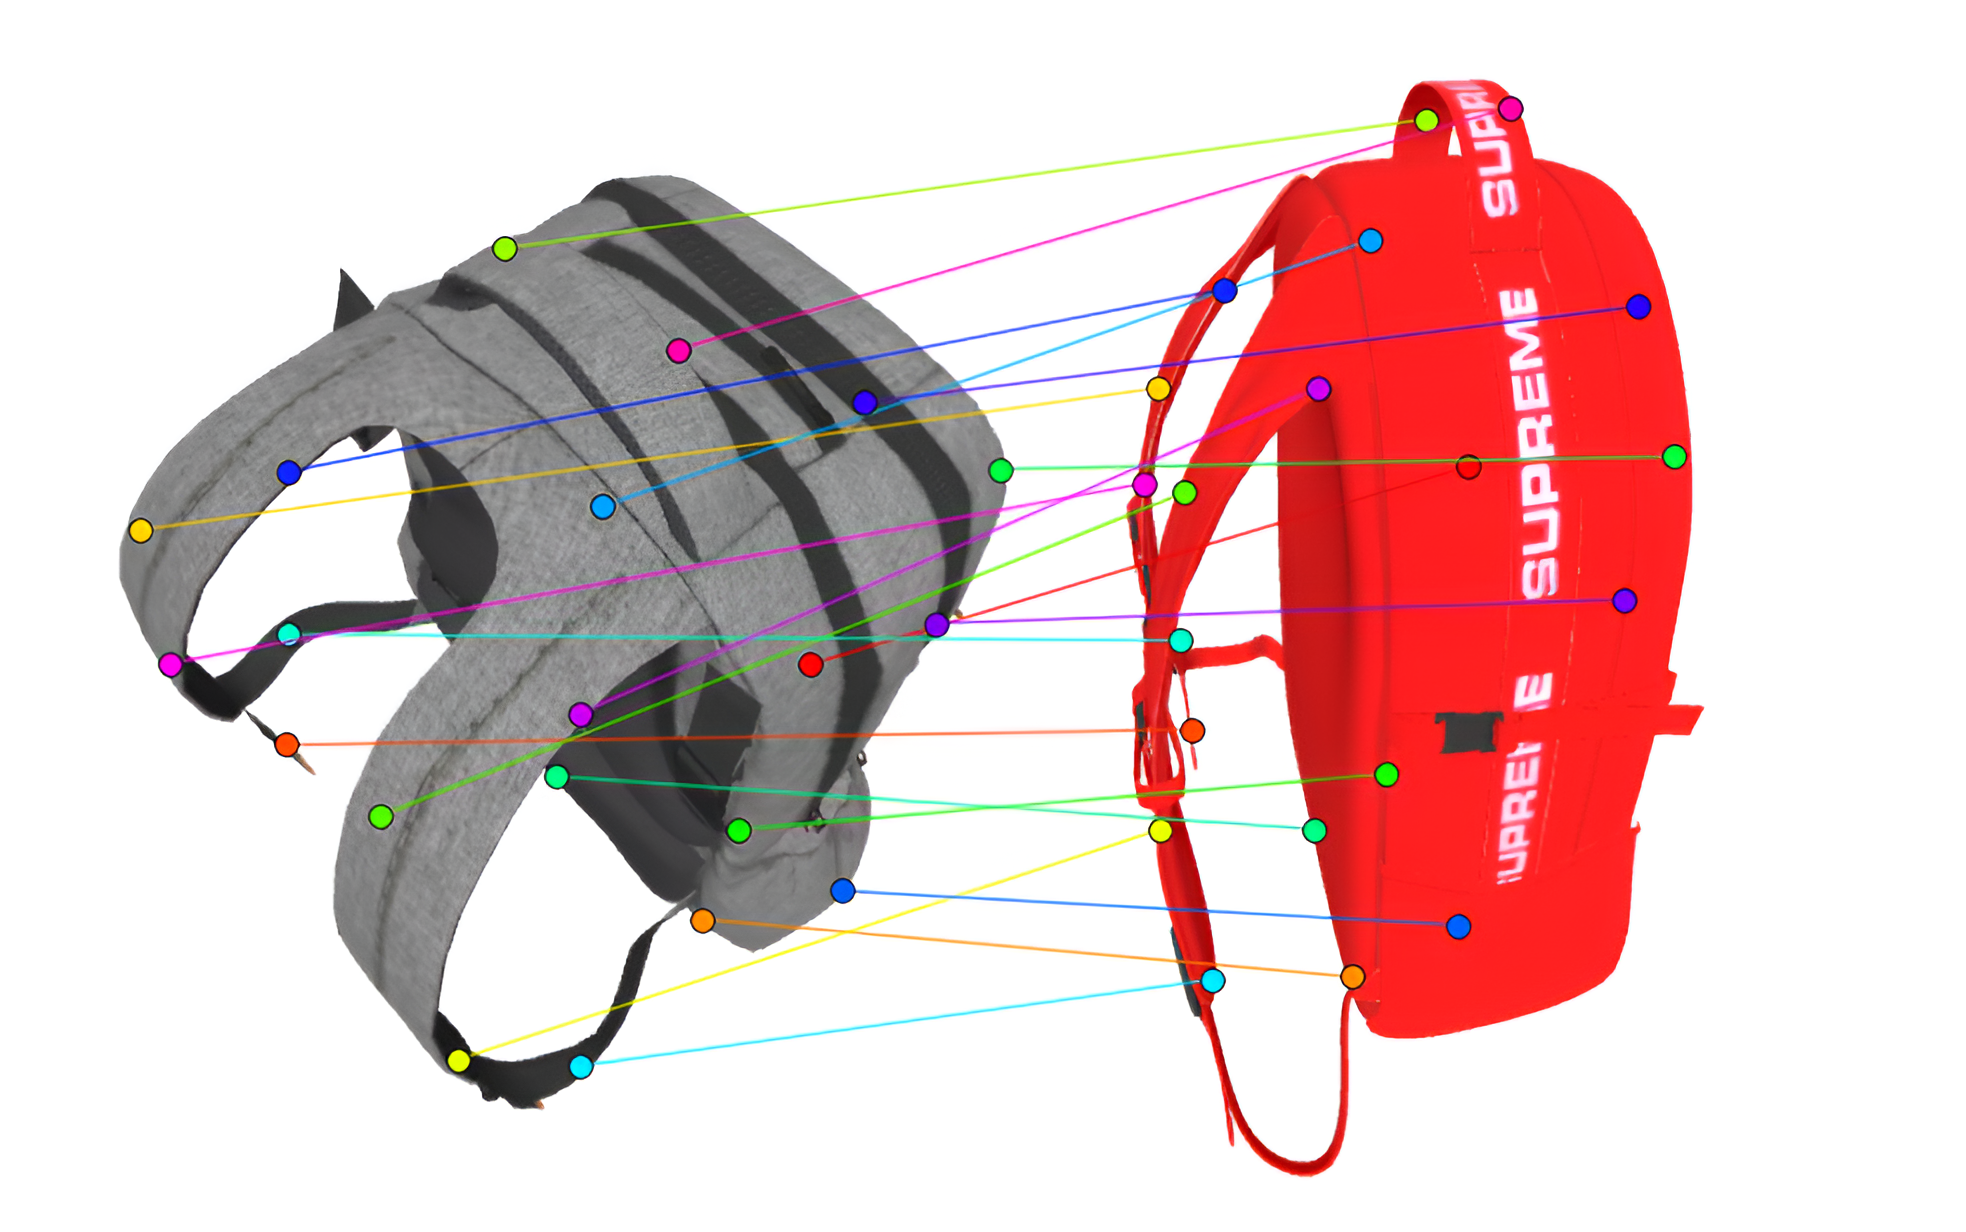
\includegraphics[width=0.92\linewidth,height=0.22\textheight,keepaspectratio,trim={0 20 70 40},clip]{figures/matching_examples/backpack_highres.png}\vspace{1mm}

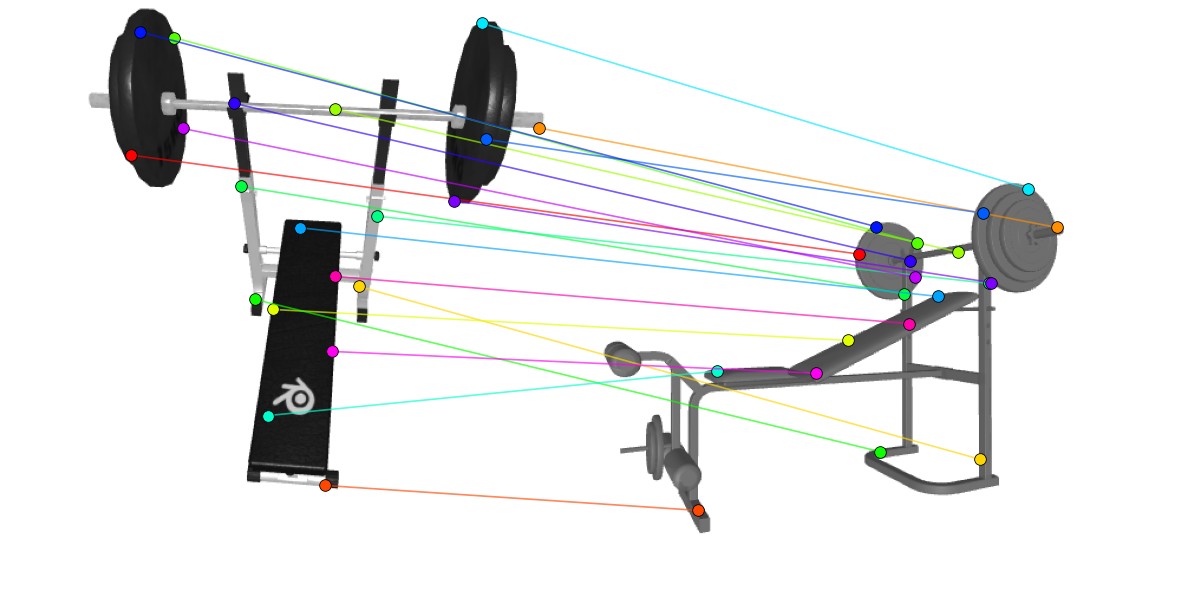
\includegraphics[width=0.92\linewidth,height=0.22\textheight,keepaspectratio,trim={0 45 50 0},clip]{figures/matching_examples/barbell.png}

\caption{
Qualitative correspondence examples on categories beyond existing correspondence benchmarks. Colors indicate sampled semantic-geometric correspondences established by our method.
}
\label{fig:new_categories_examples}
\end{figure*}

% \begin{figure*}[t]
% \centering
% 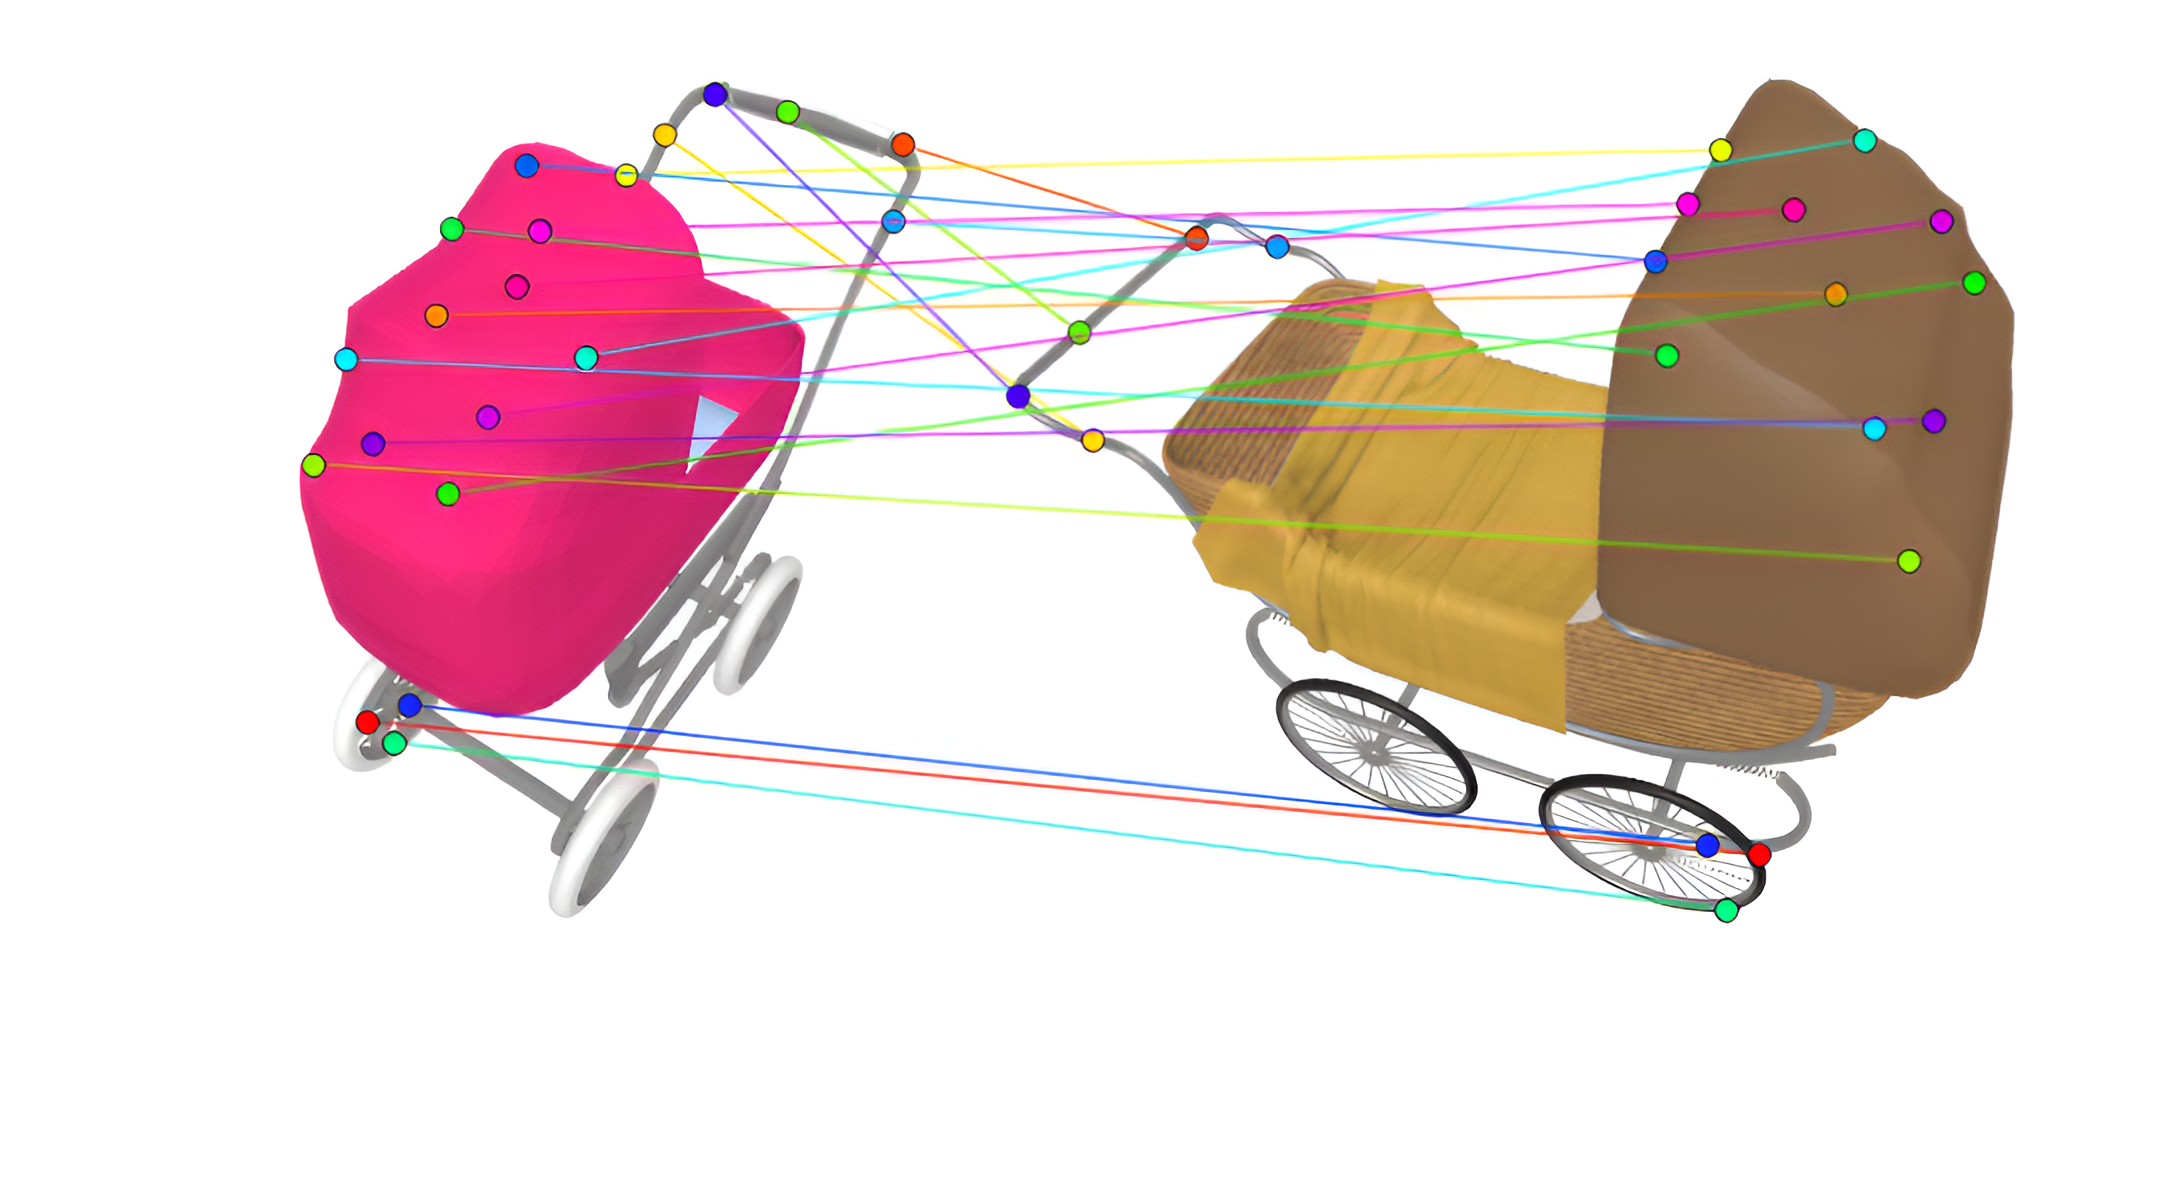
\includegraphics[width=\linewidth,height=\kpimgheight,trim={100 150 100 40},clip]{figures/matching_examples/baby_buggy_highres.png}\vfill
% % 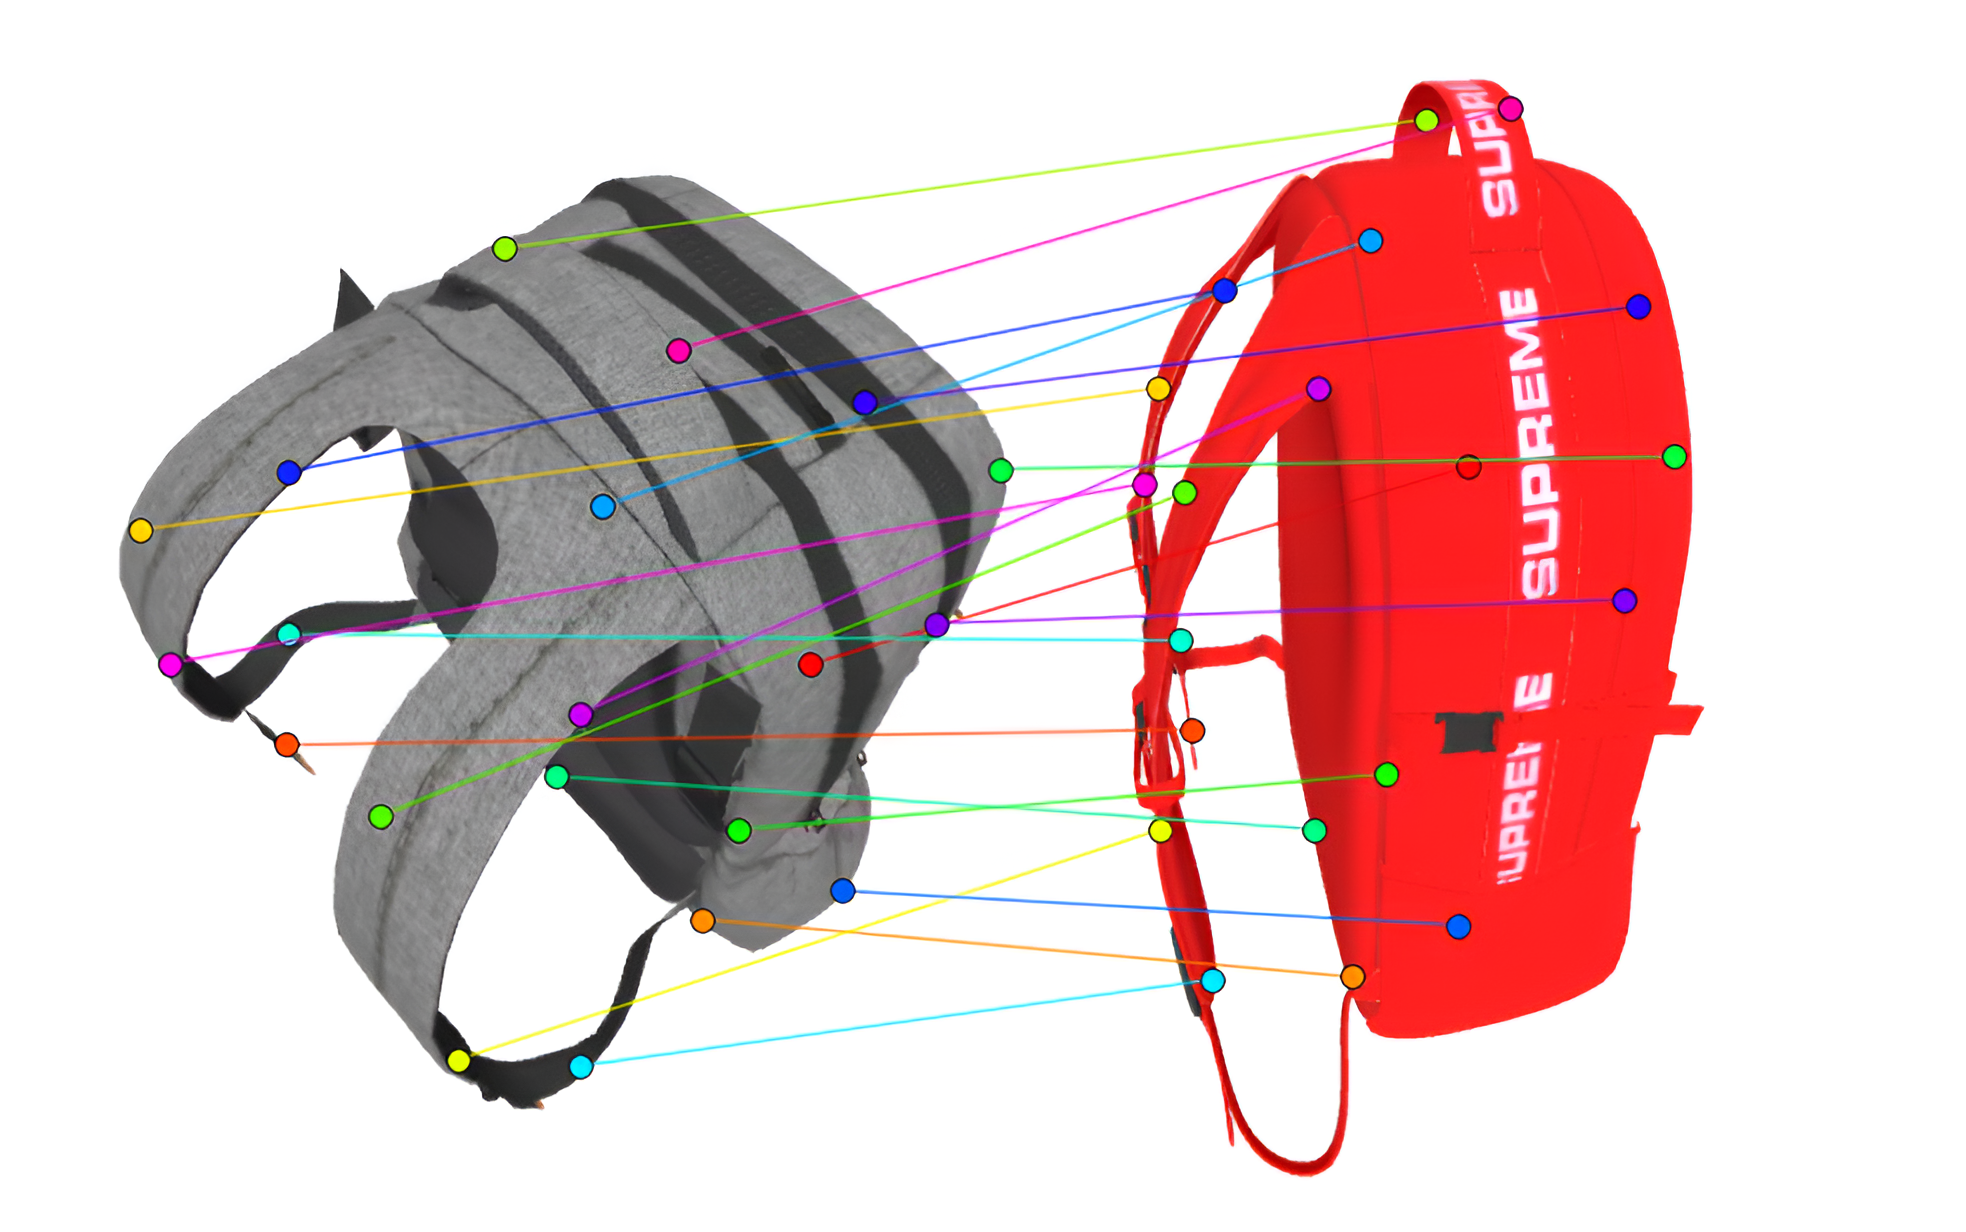
\includegraphics[width=\linewidth,height=\kpimgheight,trim={0 20 70 40},clip]{figures/matching_examples/backpack_highres.png}\vfill
% % 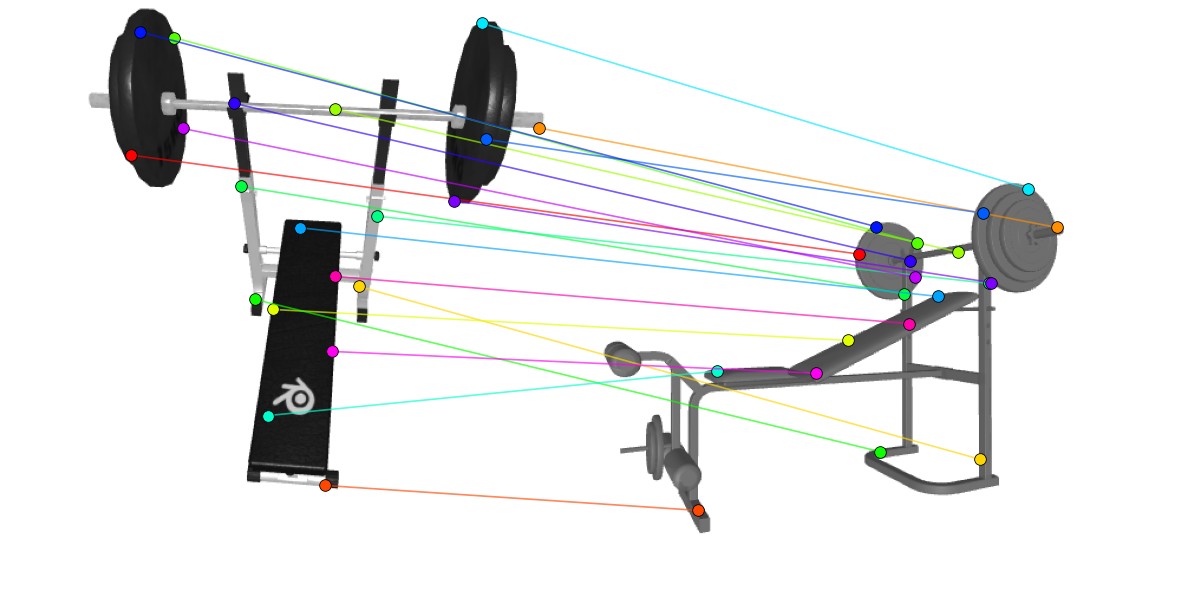
\includegraphics[width=\linewidth,height=\kpimgheight,trim={00 45 50 0},clip]{figures/matching_examples/barbell.png}
% \caption{
% Qualitative correspondence examples on categories beyond existing correspondence benchmarks. Colors indicate sampled semantic-geometric correspondences established by our method.

% We provide qualitative SPair-71k \cite{min2019spair71k} examples comparing models trained only on real SPair-71k annotations with the same models pretrained on our generated synthetic correspondences and then fine-tuned on SPair-71k. We show results for both MARCO \cite{cuttano2026marco} (see \autoref{fig:qual_marco}) and GeoAware-SC \cite{zhang2024tellingLeftFromRight} (see \autoref{fig:qual_geoaware}).


% \begin{figure*}[t]
% \centering
% \setlength{\tabcolsep}{3pt}
% \begin{tabular}{cc}
% \textbf{MARCO \cite{cuttano2026marco} Real-only} & \textbf{MARCO \cite{cuttano2026marco} Ours P.T.$\rightarrow$Real} \\
% 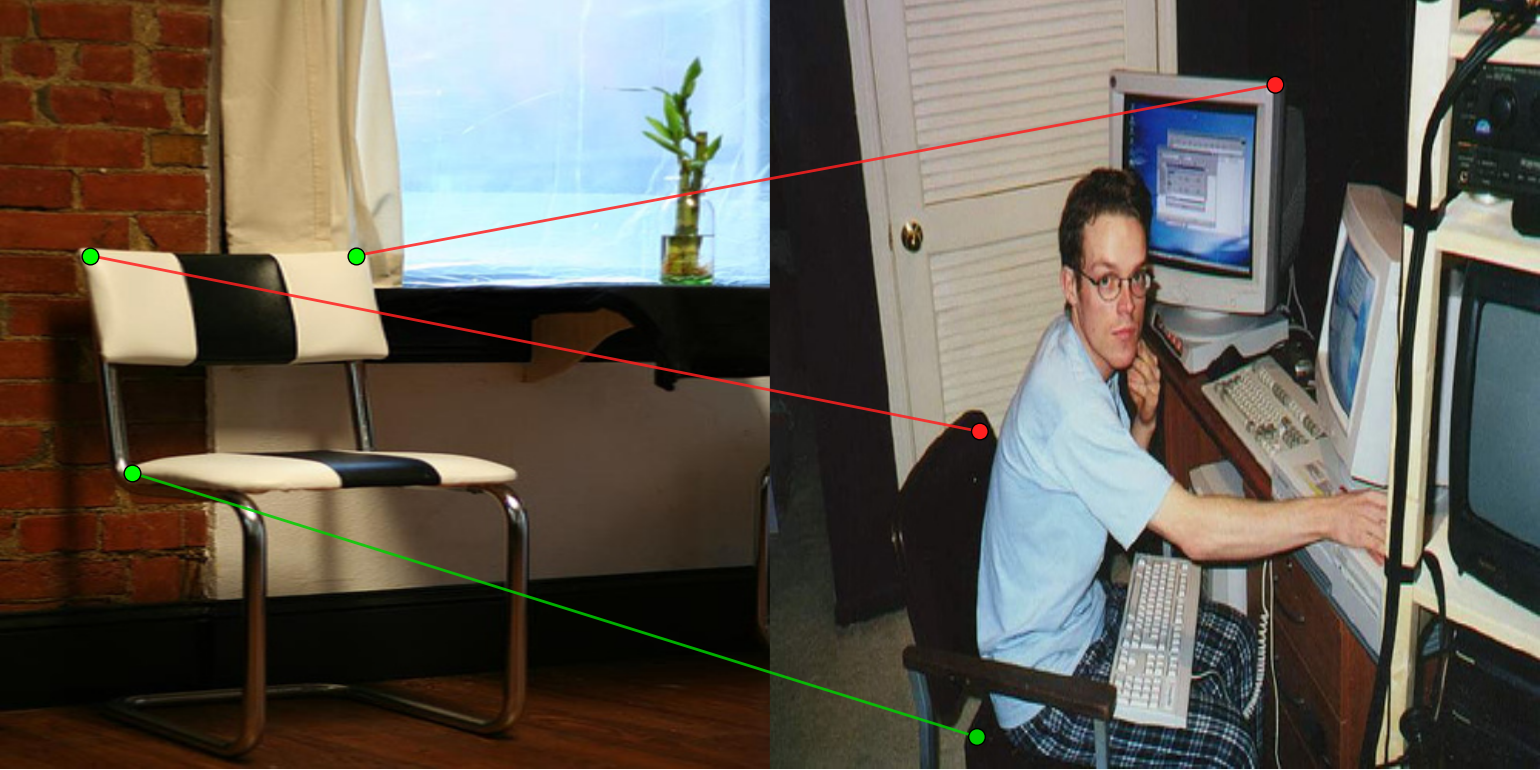
\includegraphics[width=0.48\textwidth]{figures/qualitative/marco/match_real_chair.png} &
% 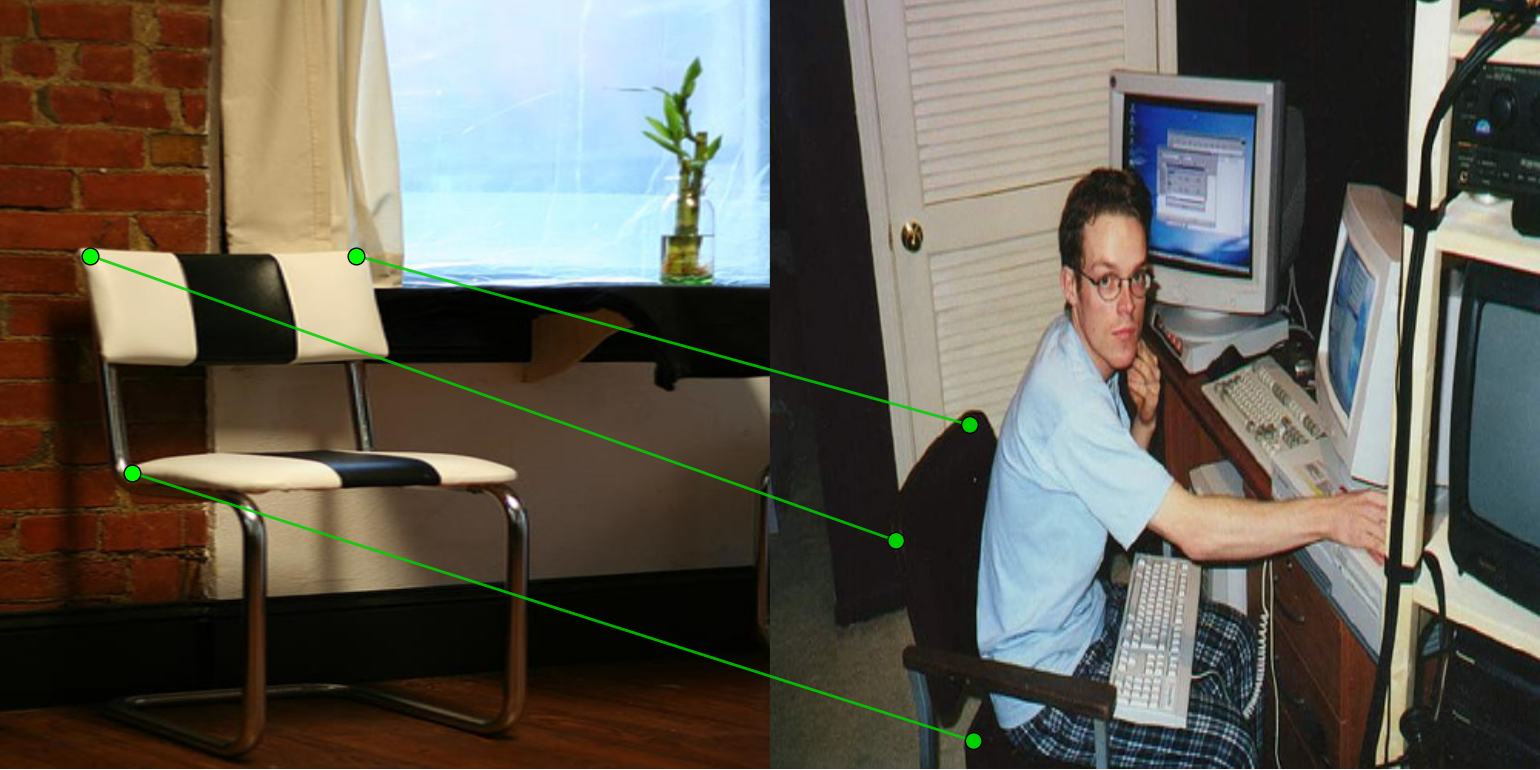
\includegraphics[width=0.48\textwidth]{figures/qualitative/marco/match_ours_chair.png} \\
% 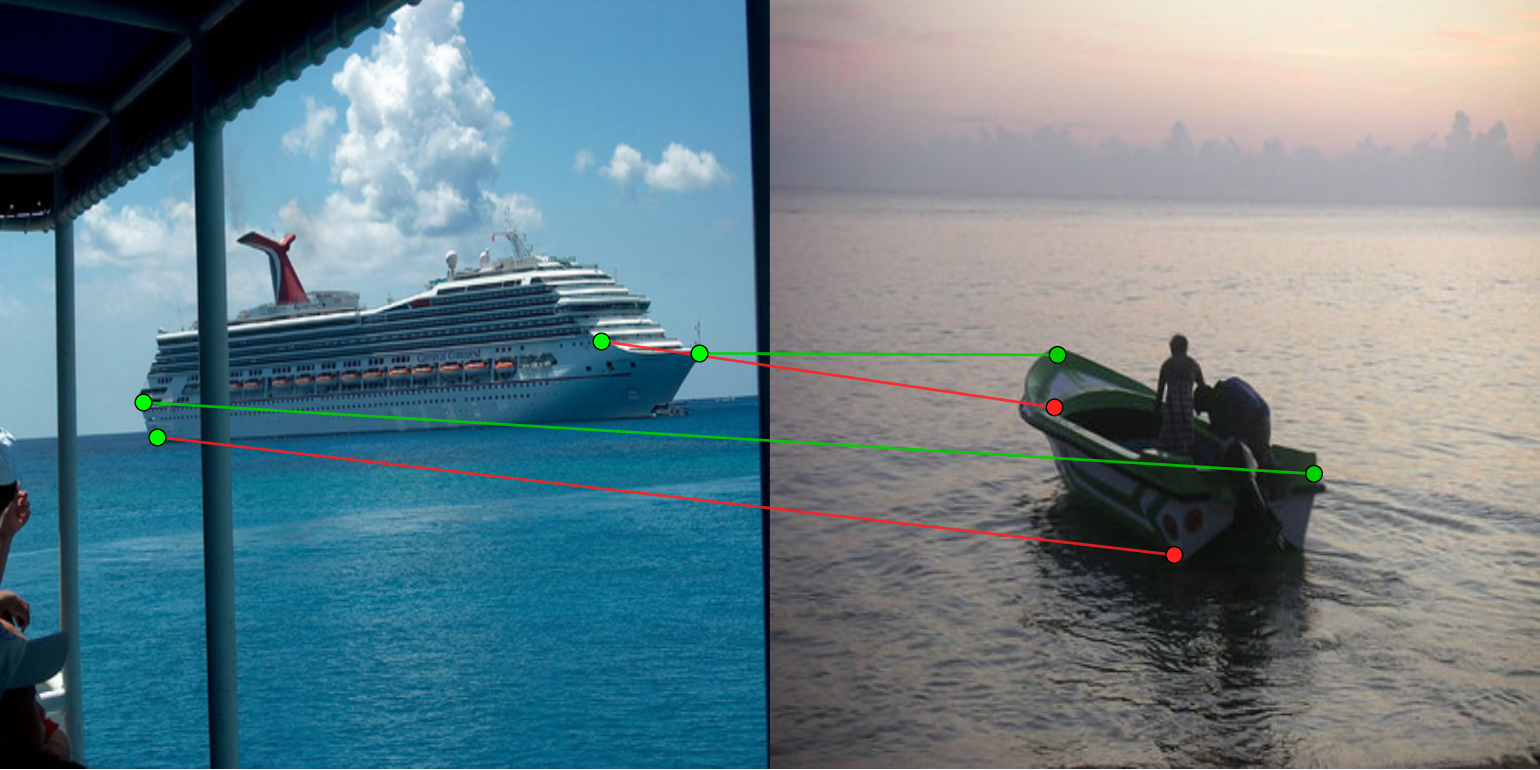
\includegraphics[width=0.48\textwidth]{figures/qualitative/marco/match_real_boat.png} &
% 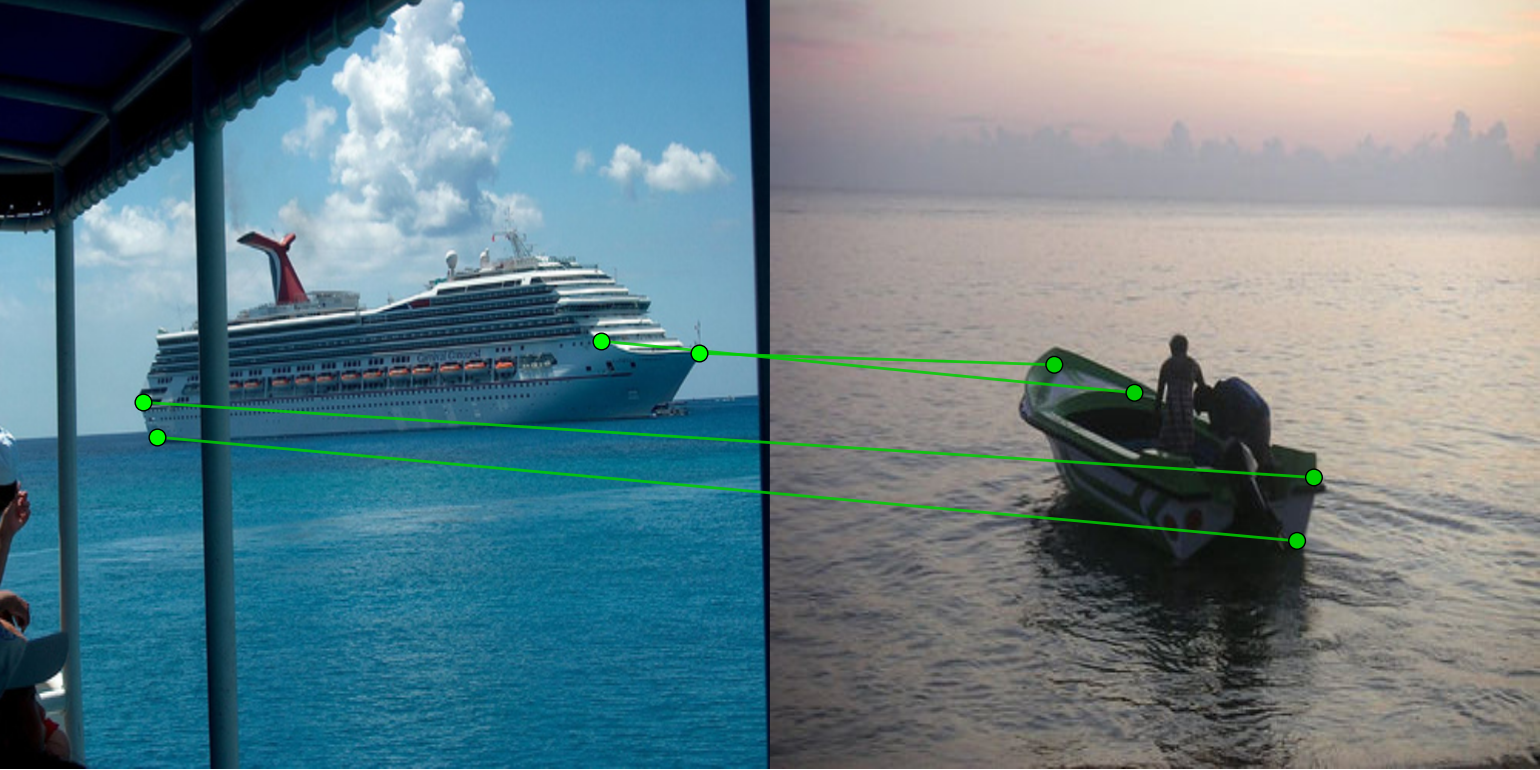
\includegraphics[width=0.48\textwidth]{figures/qualitative/marco/match_ours_boat.png} \\
% 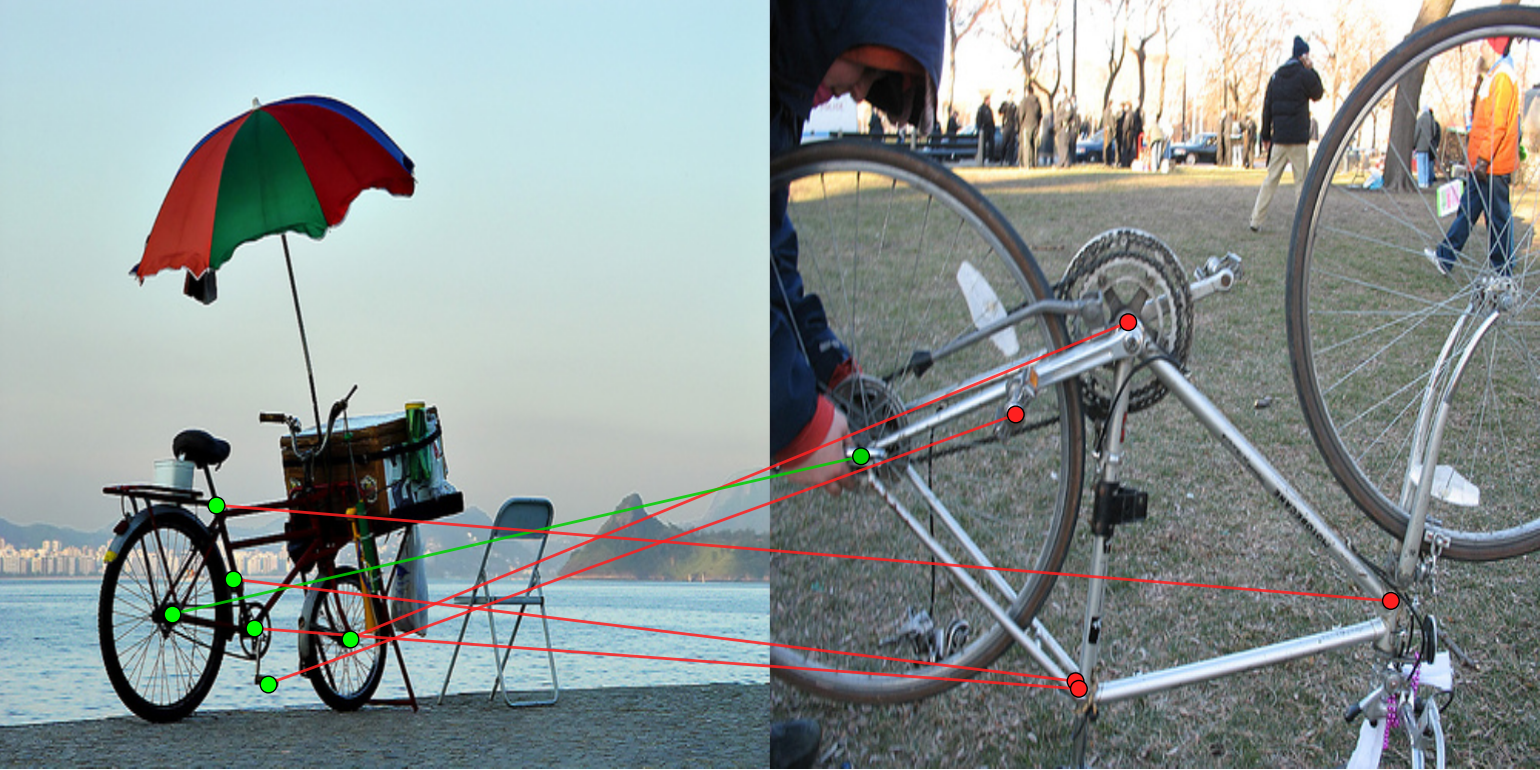
\includegraphics[width=0.48\textwidth]{figures/qualitative/marco/match_real_bicycle.png} &
% 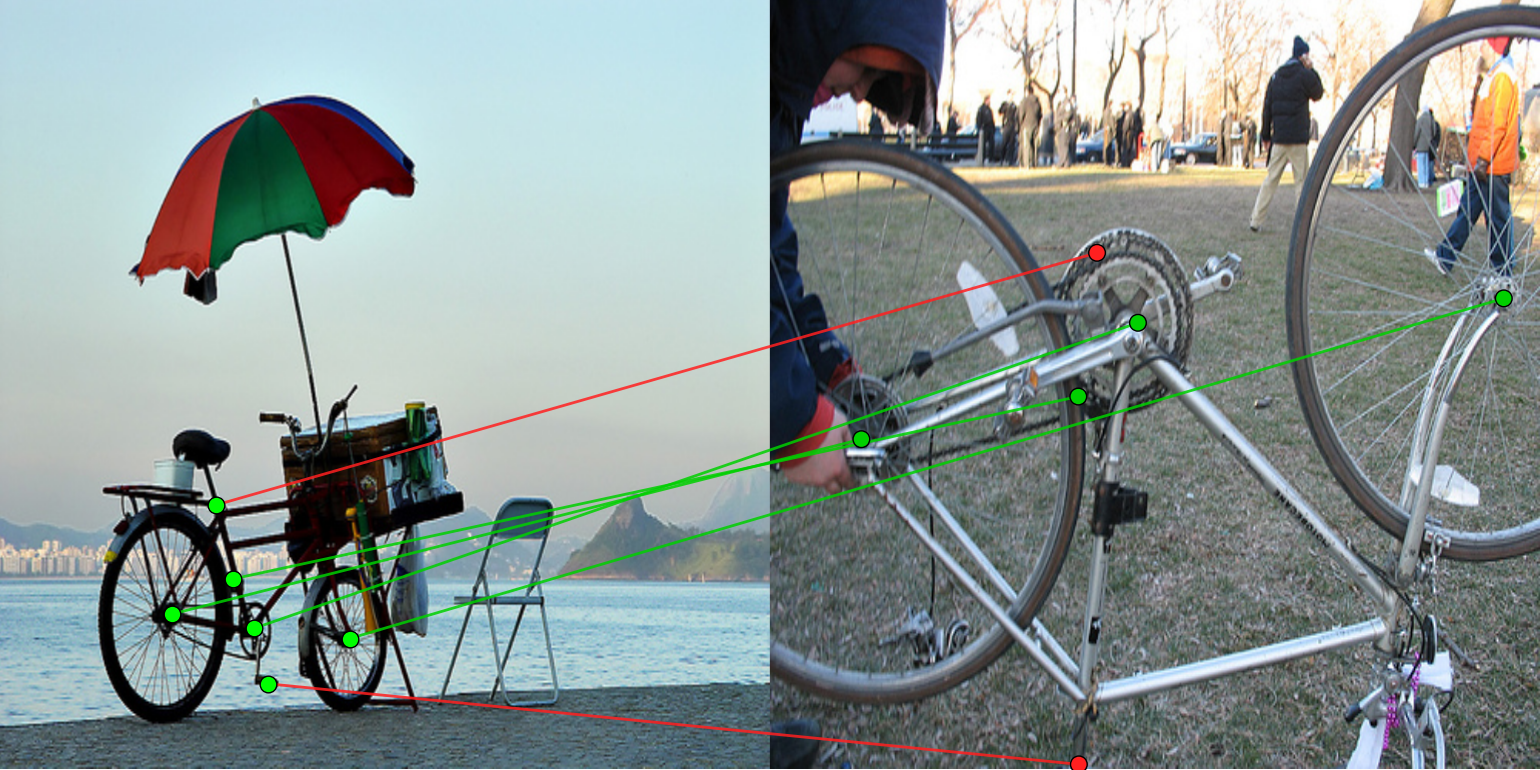
\includegraphics[width=0.48\textwidth]{figures/qualitative/marco/match_ours_bicycle.png} \\
% \end{tabular}
% \caption{\textbf{Qualitative SPair-71k \cite{min2019spair71k} results for MARCO \cite{cuttano2026marco}.}
% Each image shows a source--target pair with predicted correspondences. We compare MARCO trained on SPair-71k against MARCO pretrained on our generated correspondences and then fine-tuned on SPair-71k.}
% \label{fig:qual_marco}
% \end{figure*}


% \begin{figure*}[t]
% \centering
% \setlength{\tabcolsep}{3pt}
% \begin{tabular}{cc}
% \textbf{GeoAware-SC Real-only} & \textbf{GeoAware-SC Ours P.T.$\rightarrow$Real} \\
% 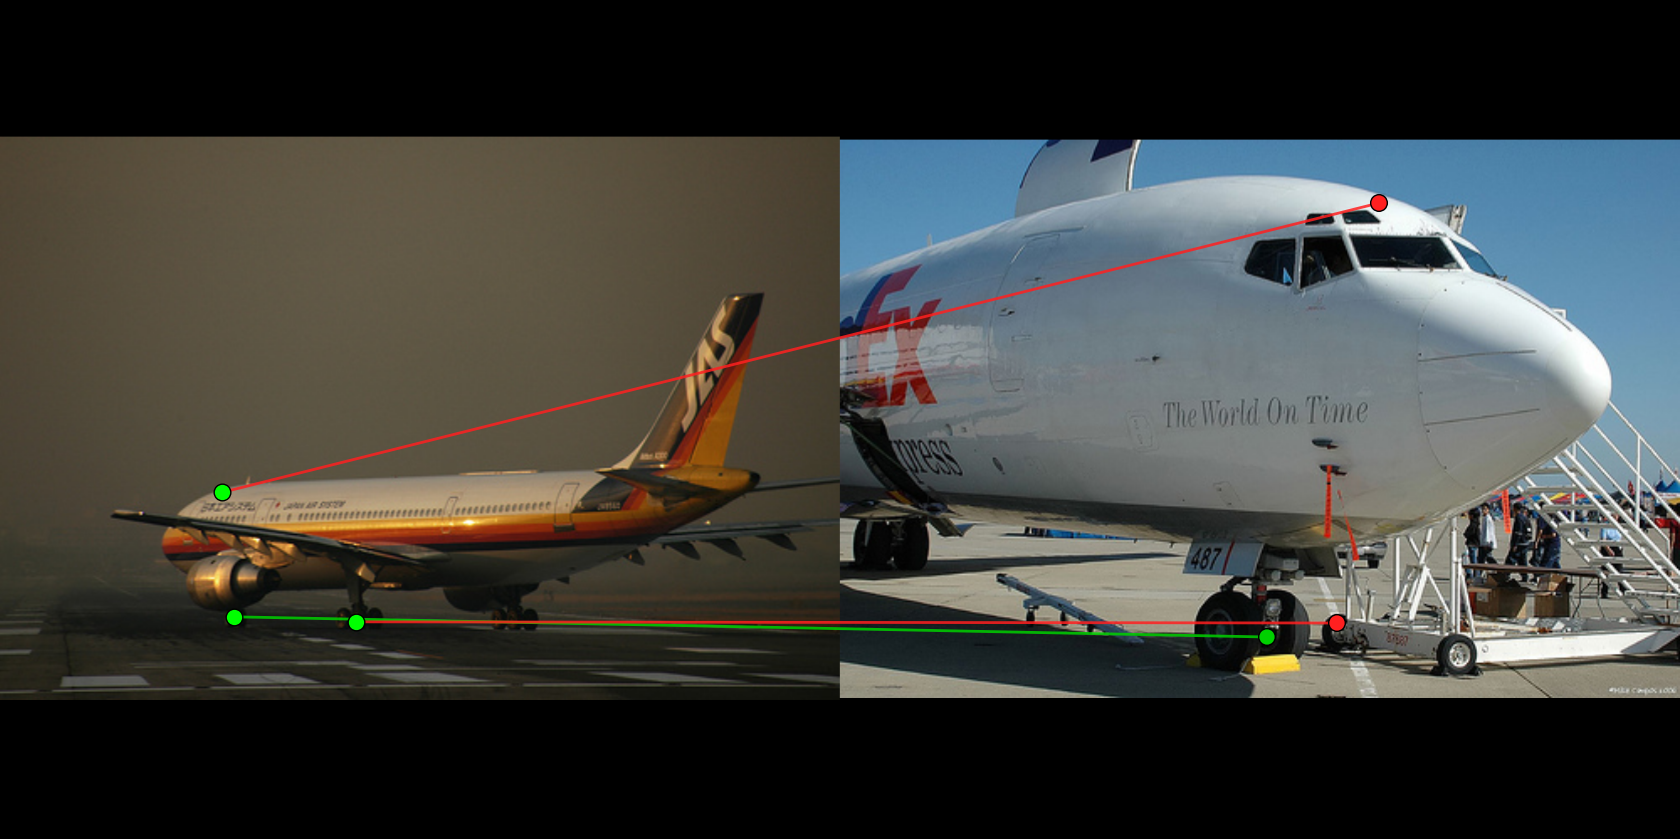
\includegraphics[width=0.48\textwidth]{figures/qualitative/geoaware/match_real_airplane.png} &
% 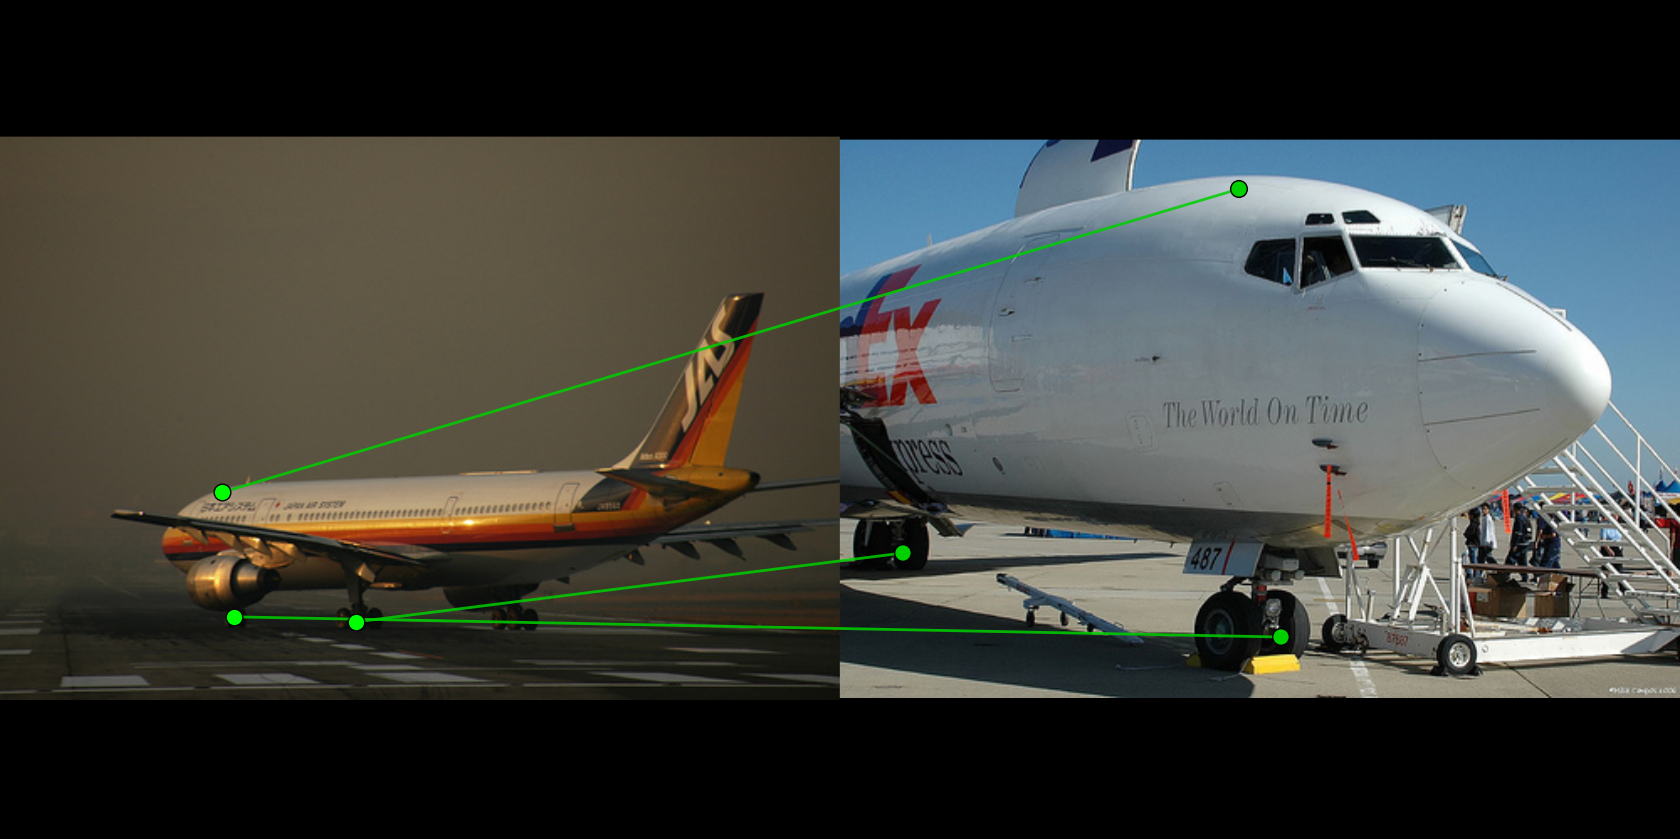
\includegraphics[width=0.48\textwidth]{figures/qualitative/geoaware/match_ours_airplane.png} \\
% 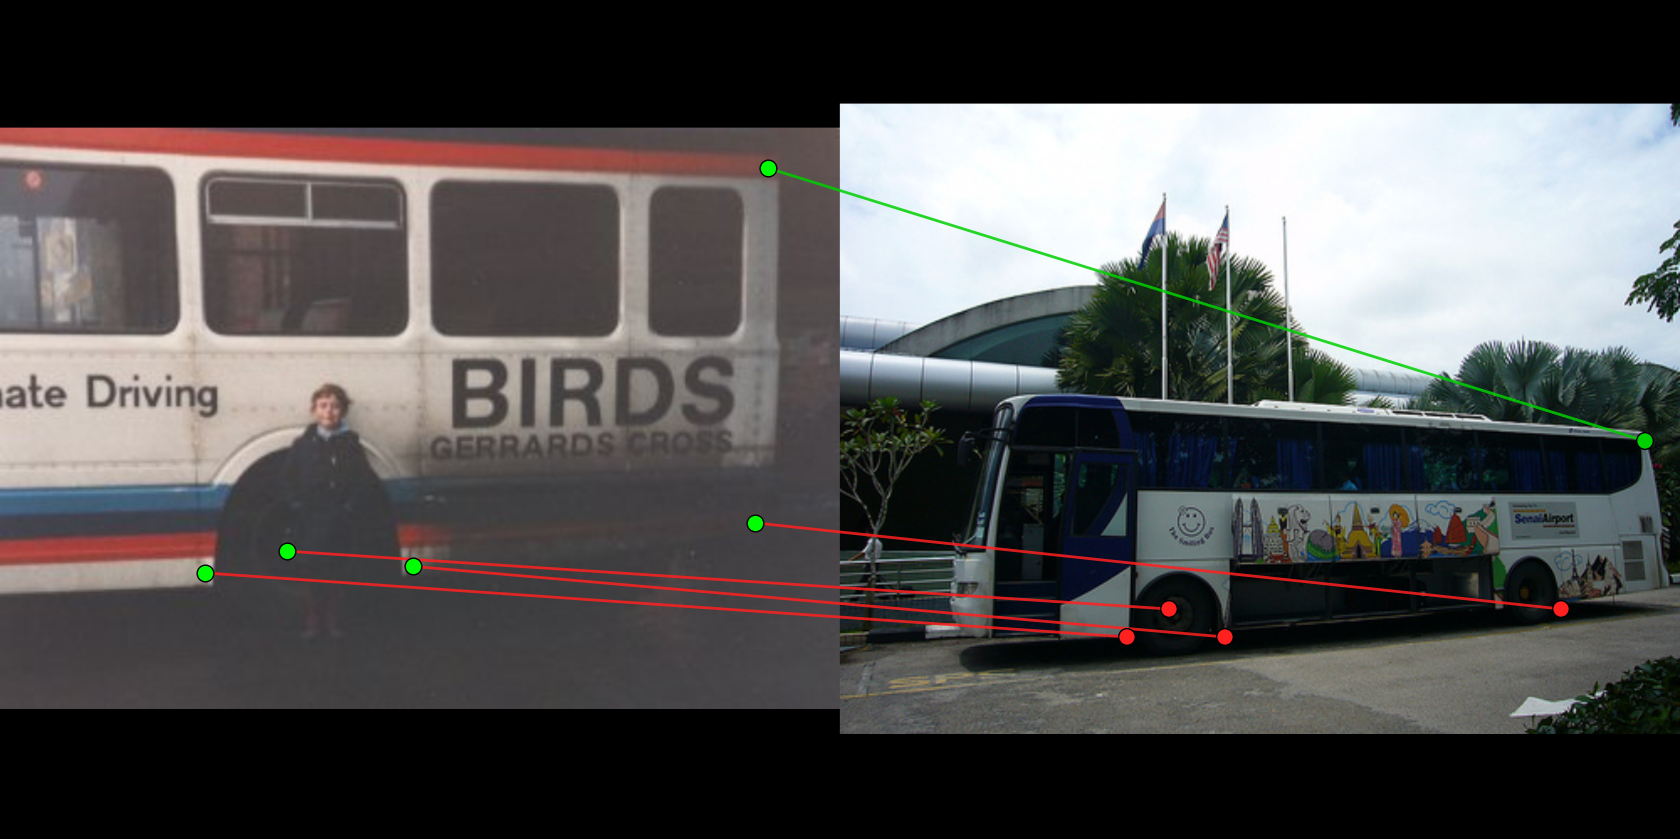
\includegraphics[width=0.48\textwidth]{figures/qualitative/geoaware/match_real_bus.png} &
% 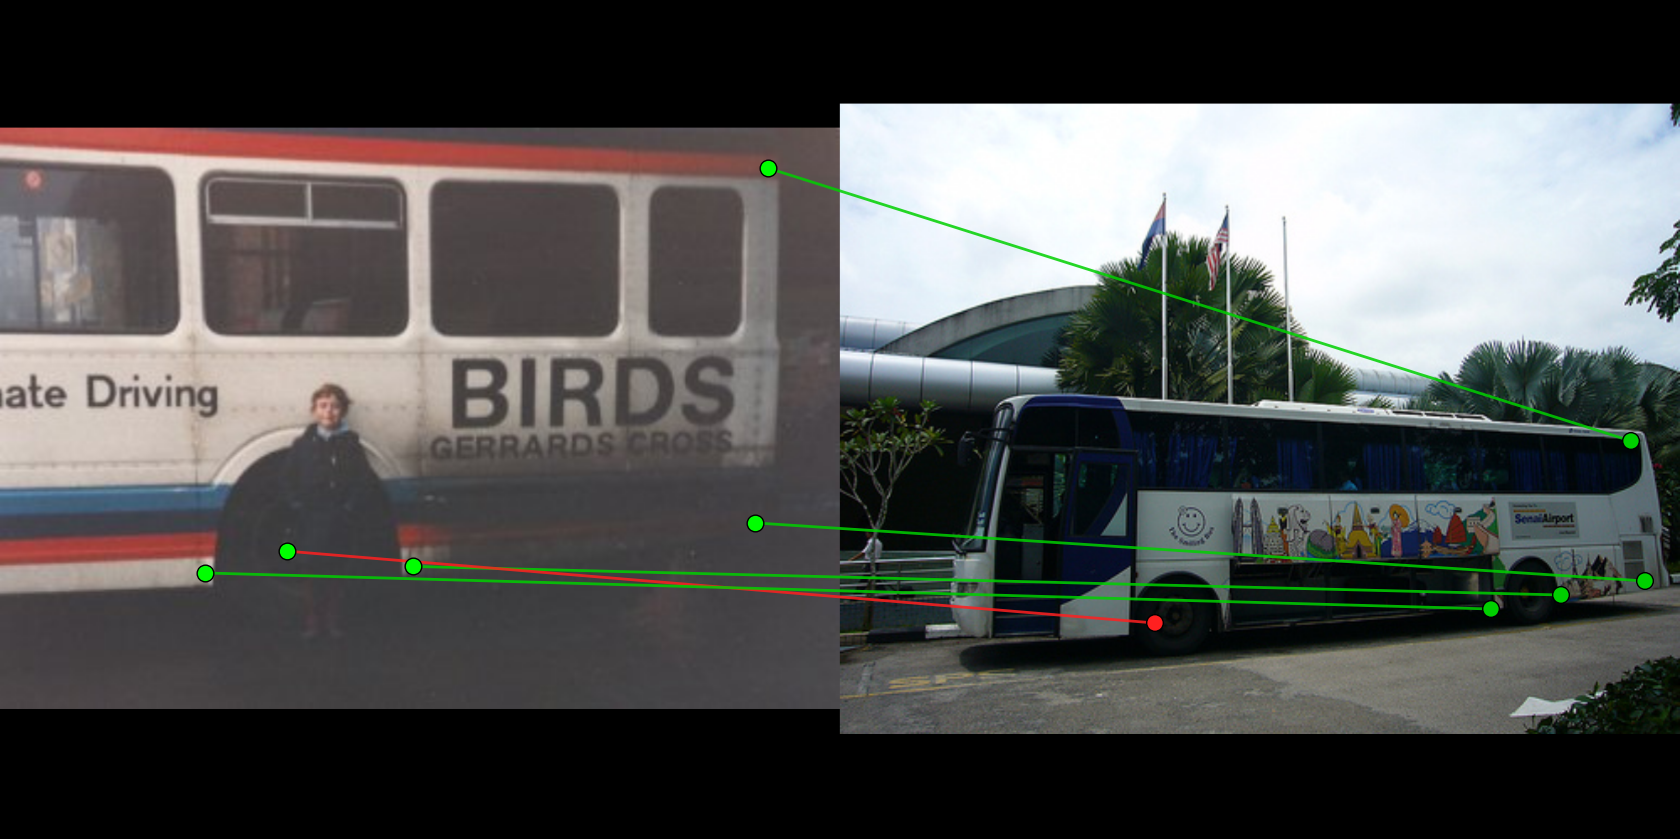
\includegraphics[width=0.48\textwidth]{figures/qualitative/geoaware/match_ours_bus.png} \\
% 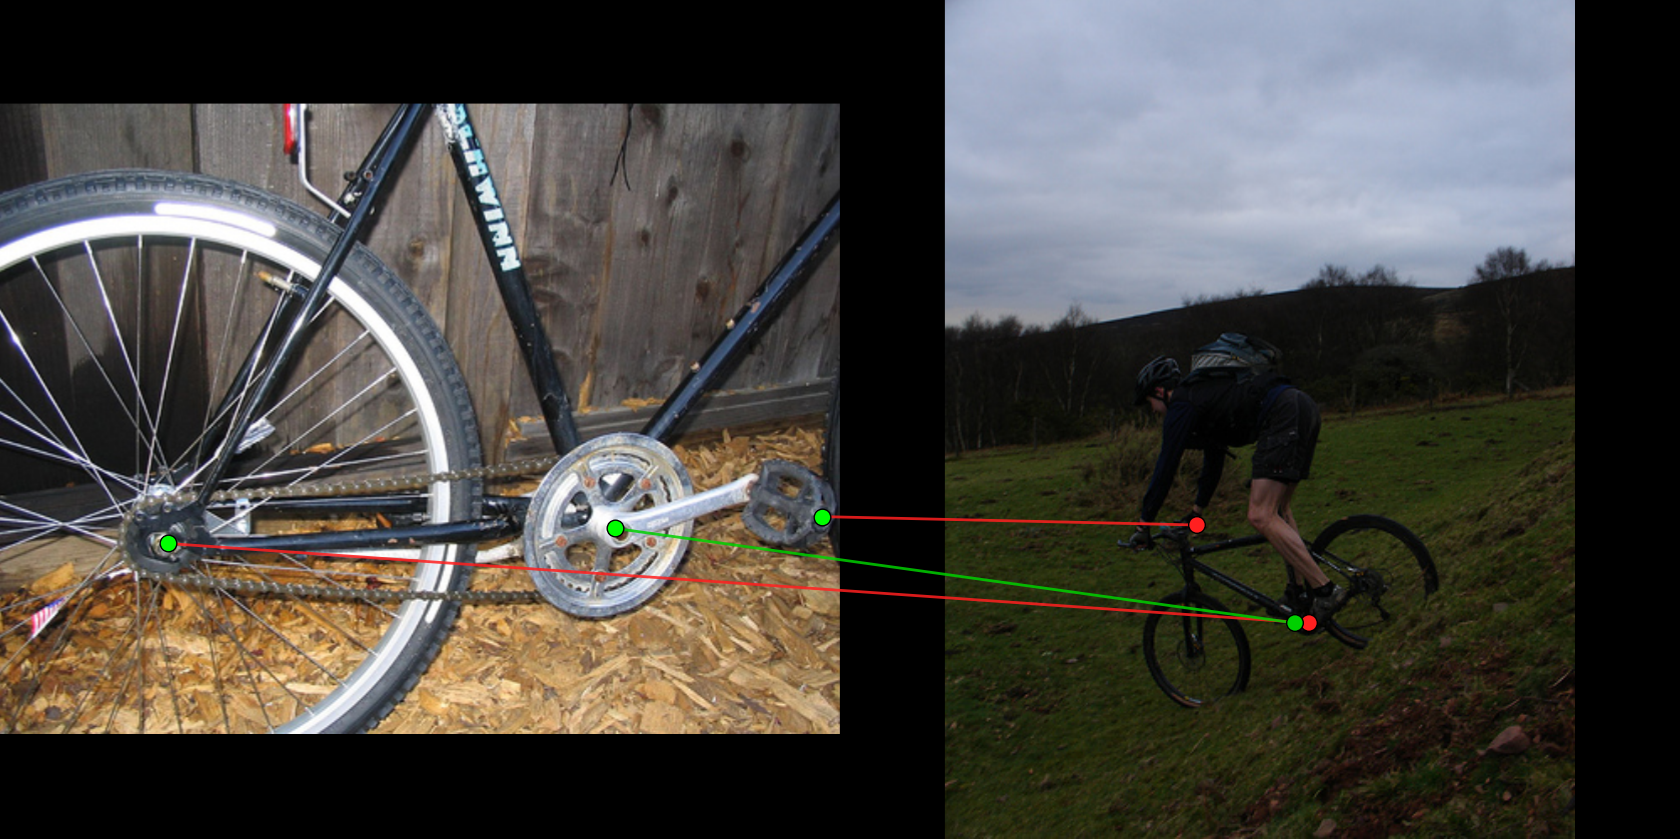
\includegraphics[width=0.48\textwidth]{figures/qualitative/geoaware/match_real_bike.png} &
% 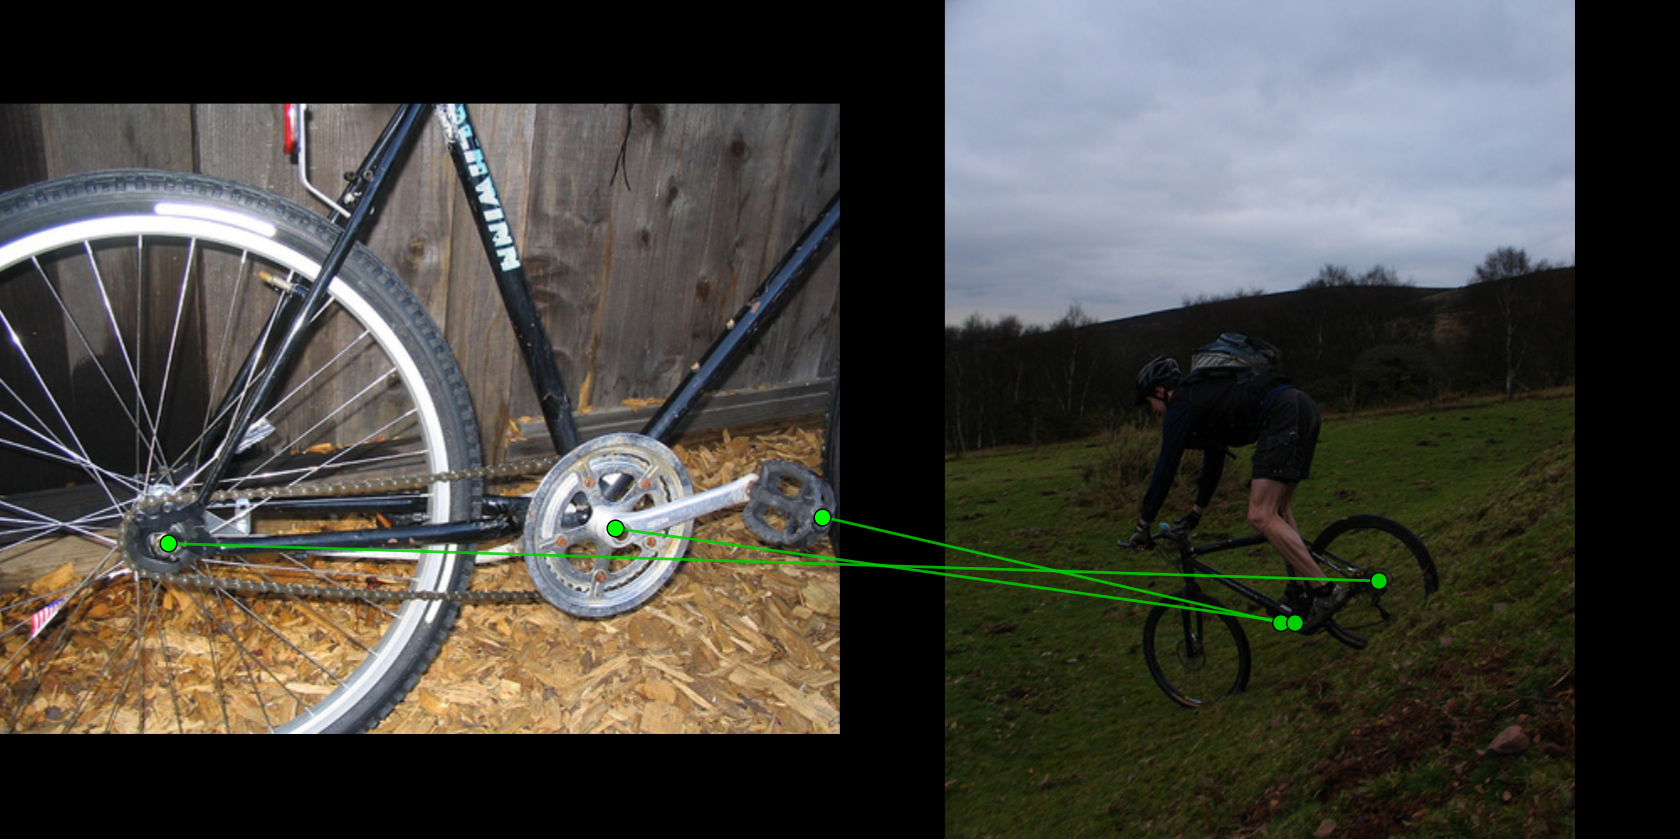
\includegraphics[width=0.48\textwidth]{figures/qualitative/geoaware/match_ours_bike.png} \\
% \end{tabular}
% \caption{\textbf{Qualitative SPair-71k \cite{min2019spair71k} results for GeoAware-SC \cite{zhang2024tellingLeftFromRight}.}
% Each image shows a source--target pair with predicted correspondences. We compare GeoAware-SC trained on SPair-71k against GeoAware-SC pretrained on our generated correspondences and then fine-tuned on SPair-71k.}
% \label{fig:qual_geoaware}
% \end{figure*}


\clearpage
\subsection{Qualitative Results on KeypointNet}

We provide qualitative correspondence results on KeypointNet \cite{you2020}, comparing our predicted correspondences against sparse human-annotated semantic keypoints. For each object pair, we use the human-annotated keypoints on the source object as queries and predict the corresponding points on the target object. As shown in \autoref{fig:keypointnet_examples}, our predictions generally align well with the human annotations across different categories. Predicted correspondences are shown in lighter colors, while the human annotations are shown in darker colors. Red lines connect each prediction to its corresponding ground-truth annotation.

We further show examples with strong agreement in \autoref{fig:keypointnet_strong_overlap}. The close overlap between our predictions and the human annotations indicates that our generated correspondences are highly consistent with the sparse semantic keypoints used for evaluation.

\begin{figure}[h]
    \centering

    \begin{subfigure}[b]{0.48\linewidth}
        \centering
        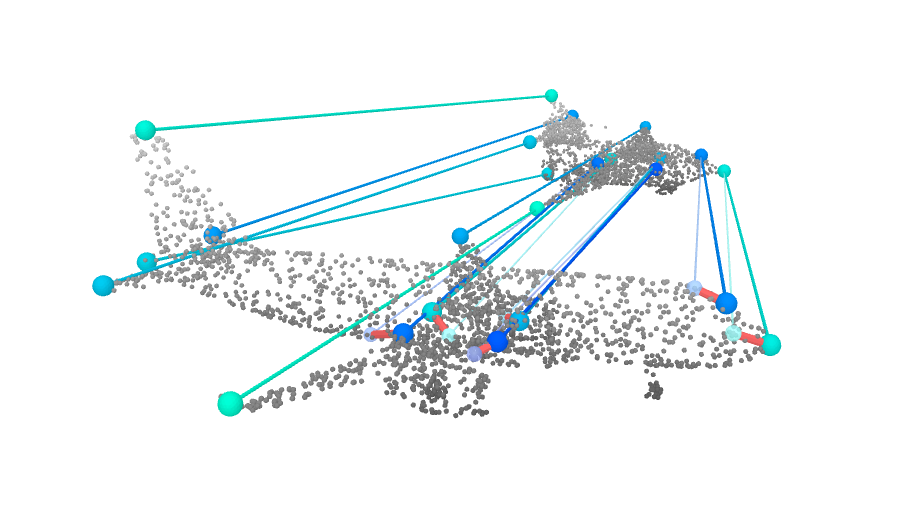
\includegraphics[width=\linewidth]{sup_mat/figures/airplane_top15_464a8718_x_dfa36bff_yaw-253p84_pitch76p57.png}
        \caption{Airplanes}
        \label{fig:example_a}
    \end{subfigure}
    \hfill
    \begin{subfigure}[b]{0.48\linewidth}
        \centering
        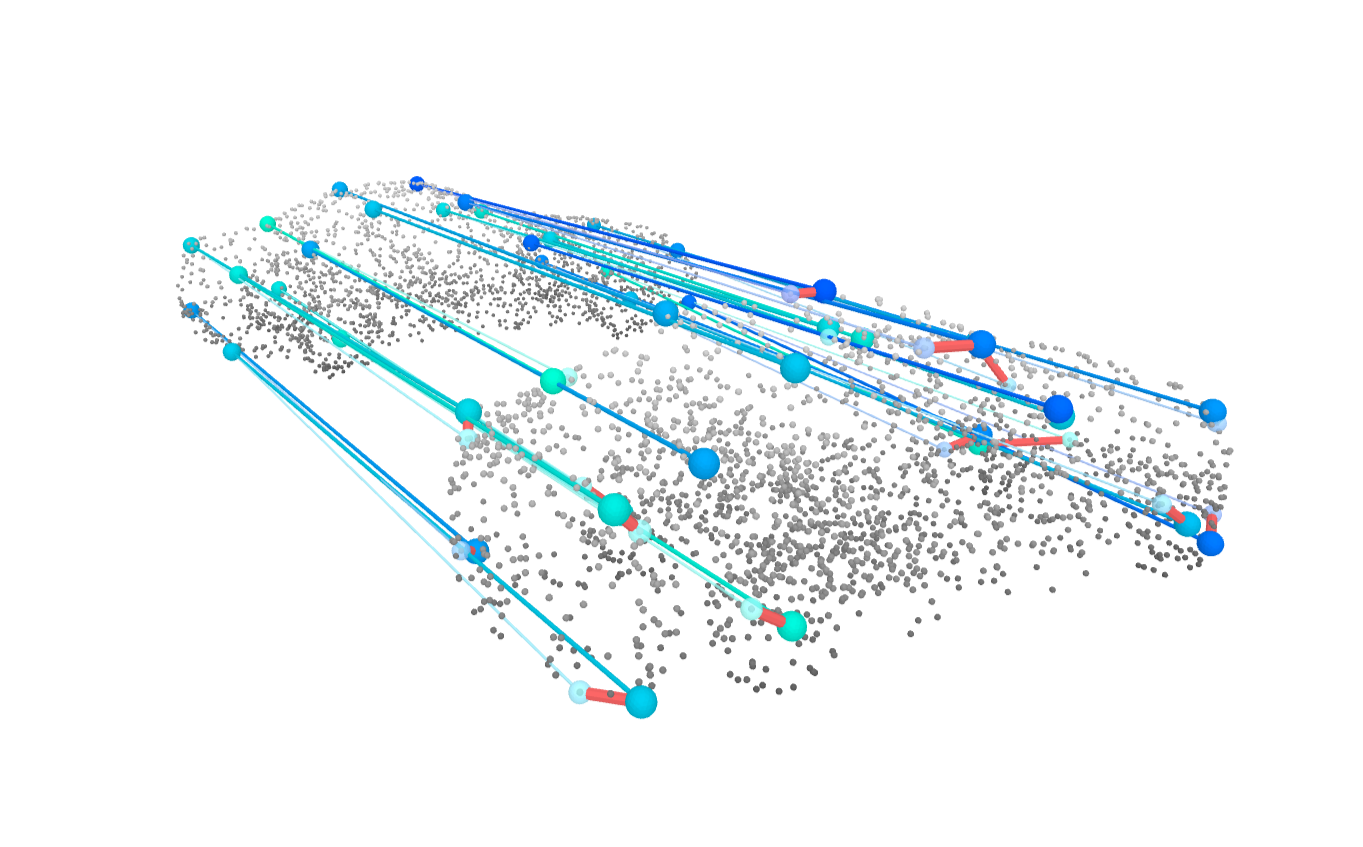
\includegraphics[width=\linewidth]{sup_mat/figures/car_top02_119033fe_x_1836f75b_yaw-298p07_pitch74p22.png}
        \caption{Cars}
        \label{fig:example_b}
    \end{subfigure}

    \caption{\textbf{Qualitative correspondence results on KeypointNet \cite{you2020}}
    We compare our predicted correspondences with human-annotated keypoints on the target object. Predicted correspondences are shown in lighter colors, while human annotations are shown in darker colors. Red lines connect each prediction to its corresponding ground-truth annotation, visualizing the localization difference between them.}
    \label{fig:keypointnet_examples}
\end{figure}

\begin{figure}[h]
    \centering

    \begin{subfigure}[b]{0.45\linewidth}
        \centering
        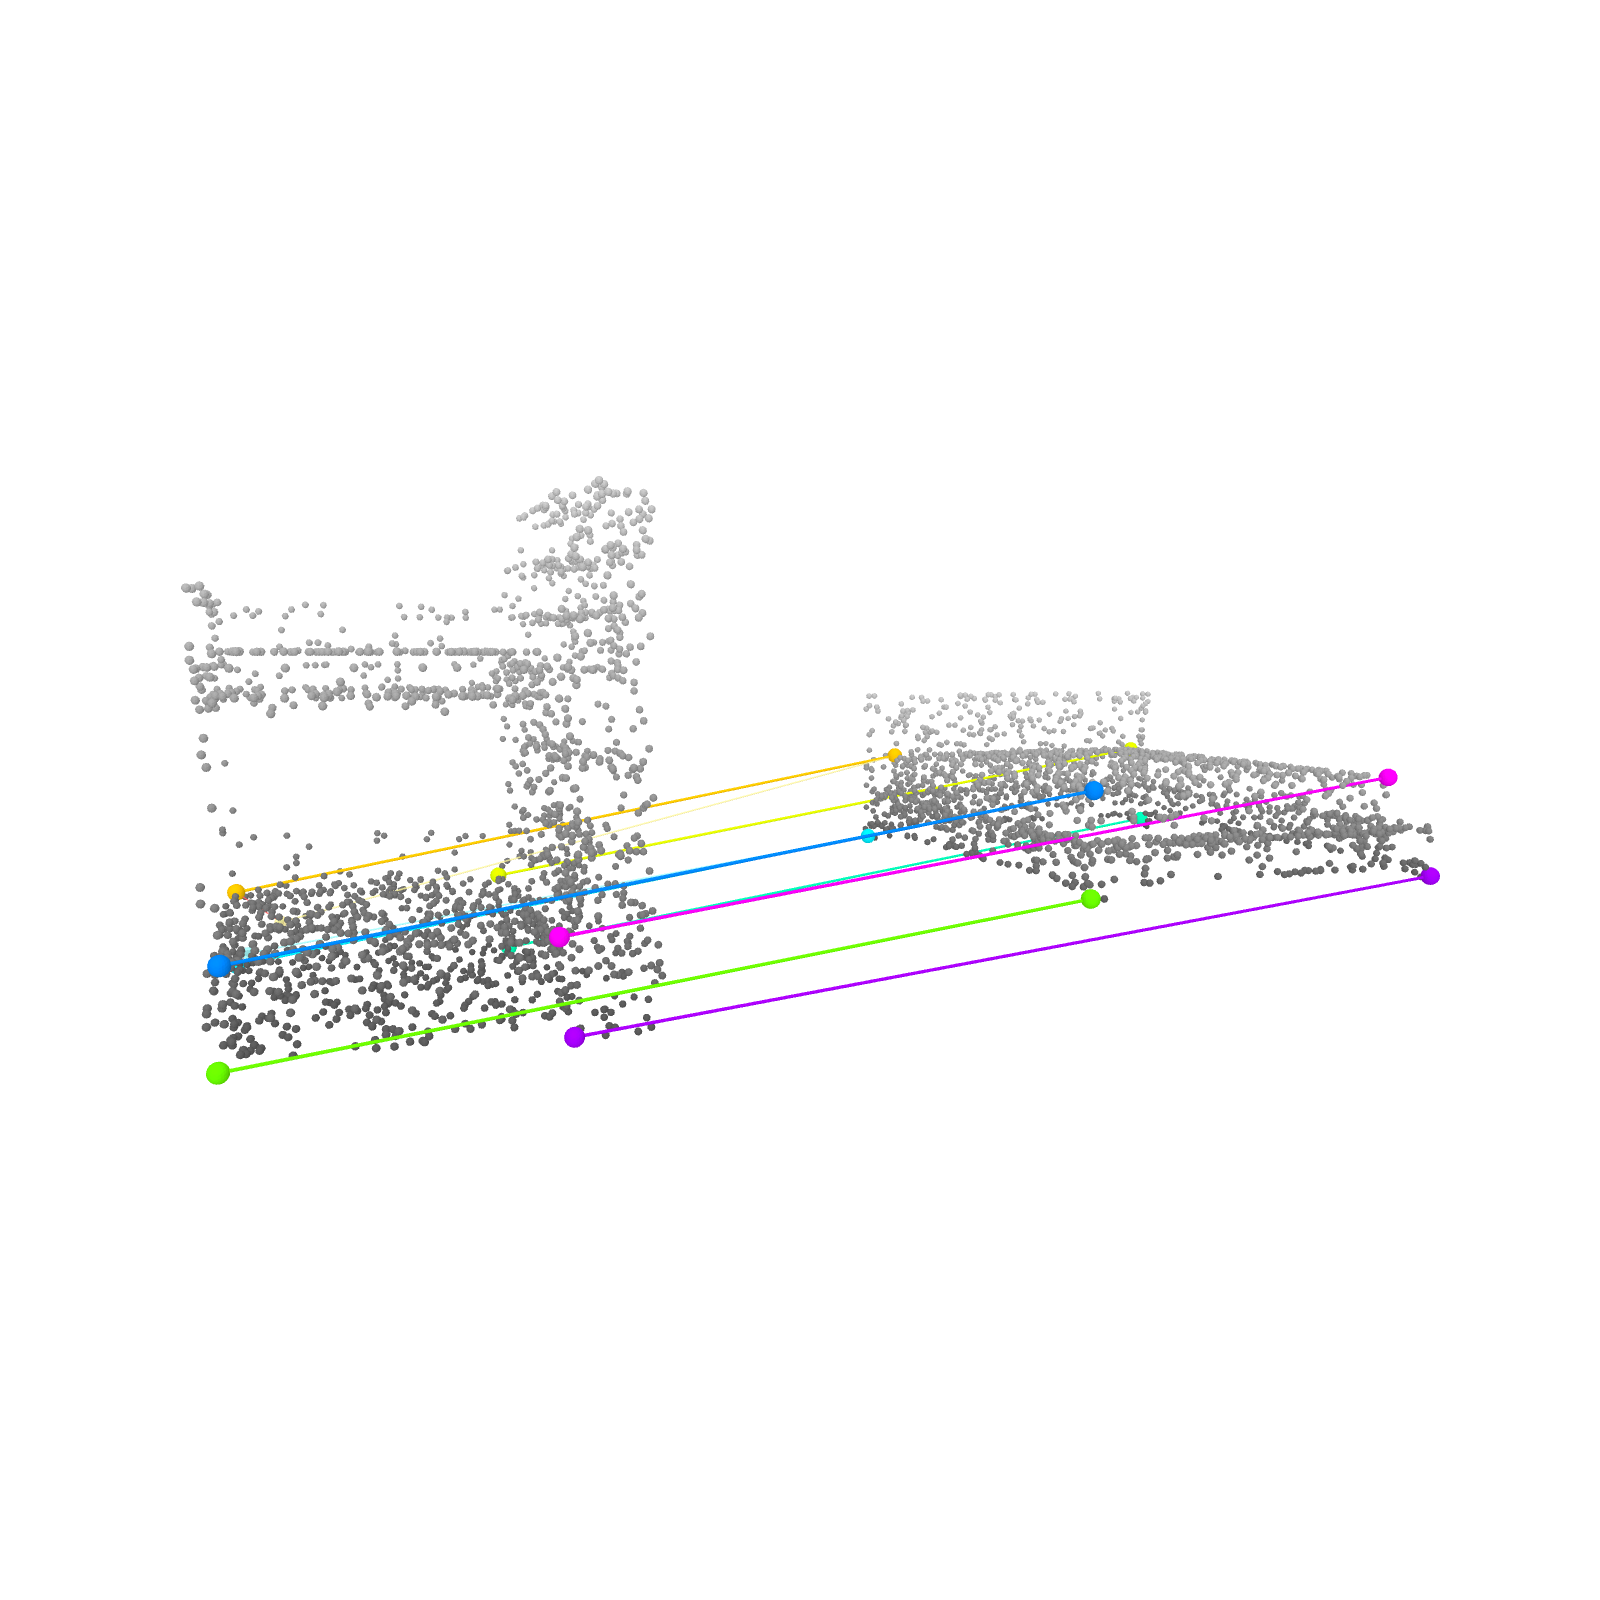
\includegraphics[trim={10 350 10 400},clip,width=\linewidth,height=\linewidth,keepaspectratio]{sup_mat/figures/bed_top11_ac97ffc6_x_e2532c6b_yaw-200p22_pitch84p01.png}
        \caption{Bed}
        \label{fig:square_bed}
    \end{subfigure}
    \hfill
    \begin{subfigure}[b]{0.45\linewidth}
        \centering
        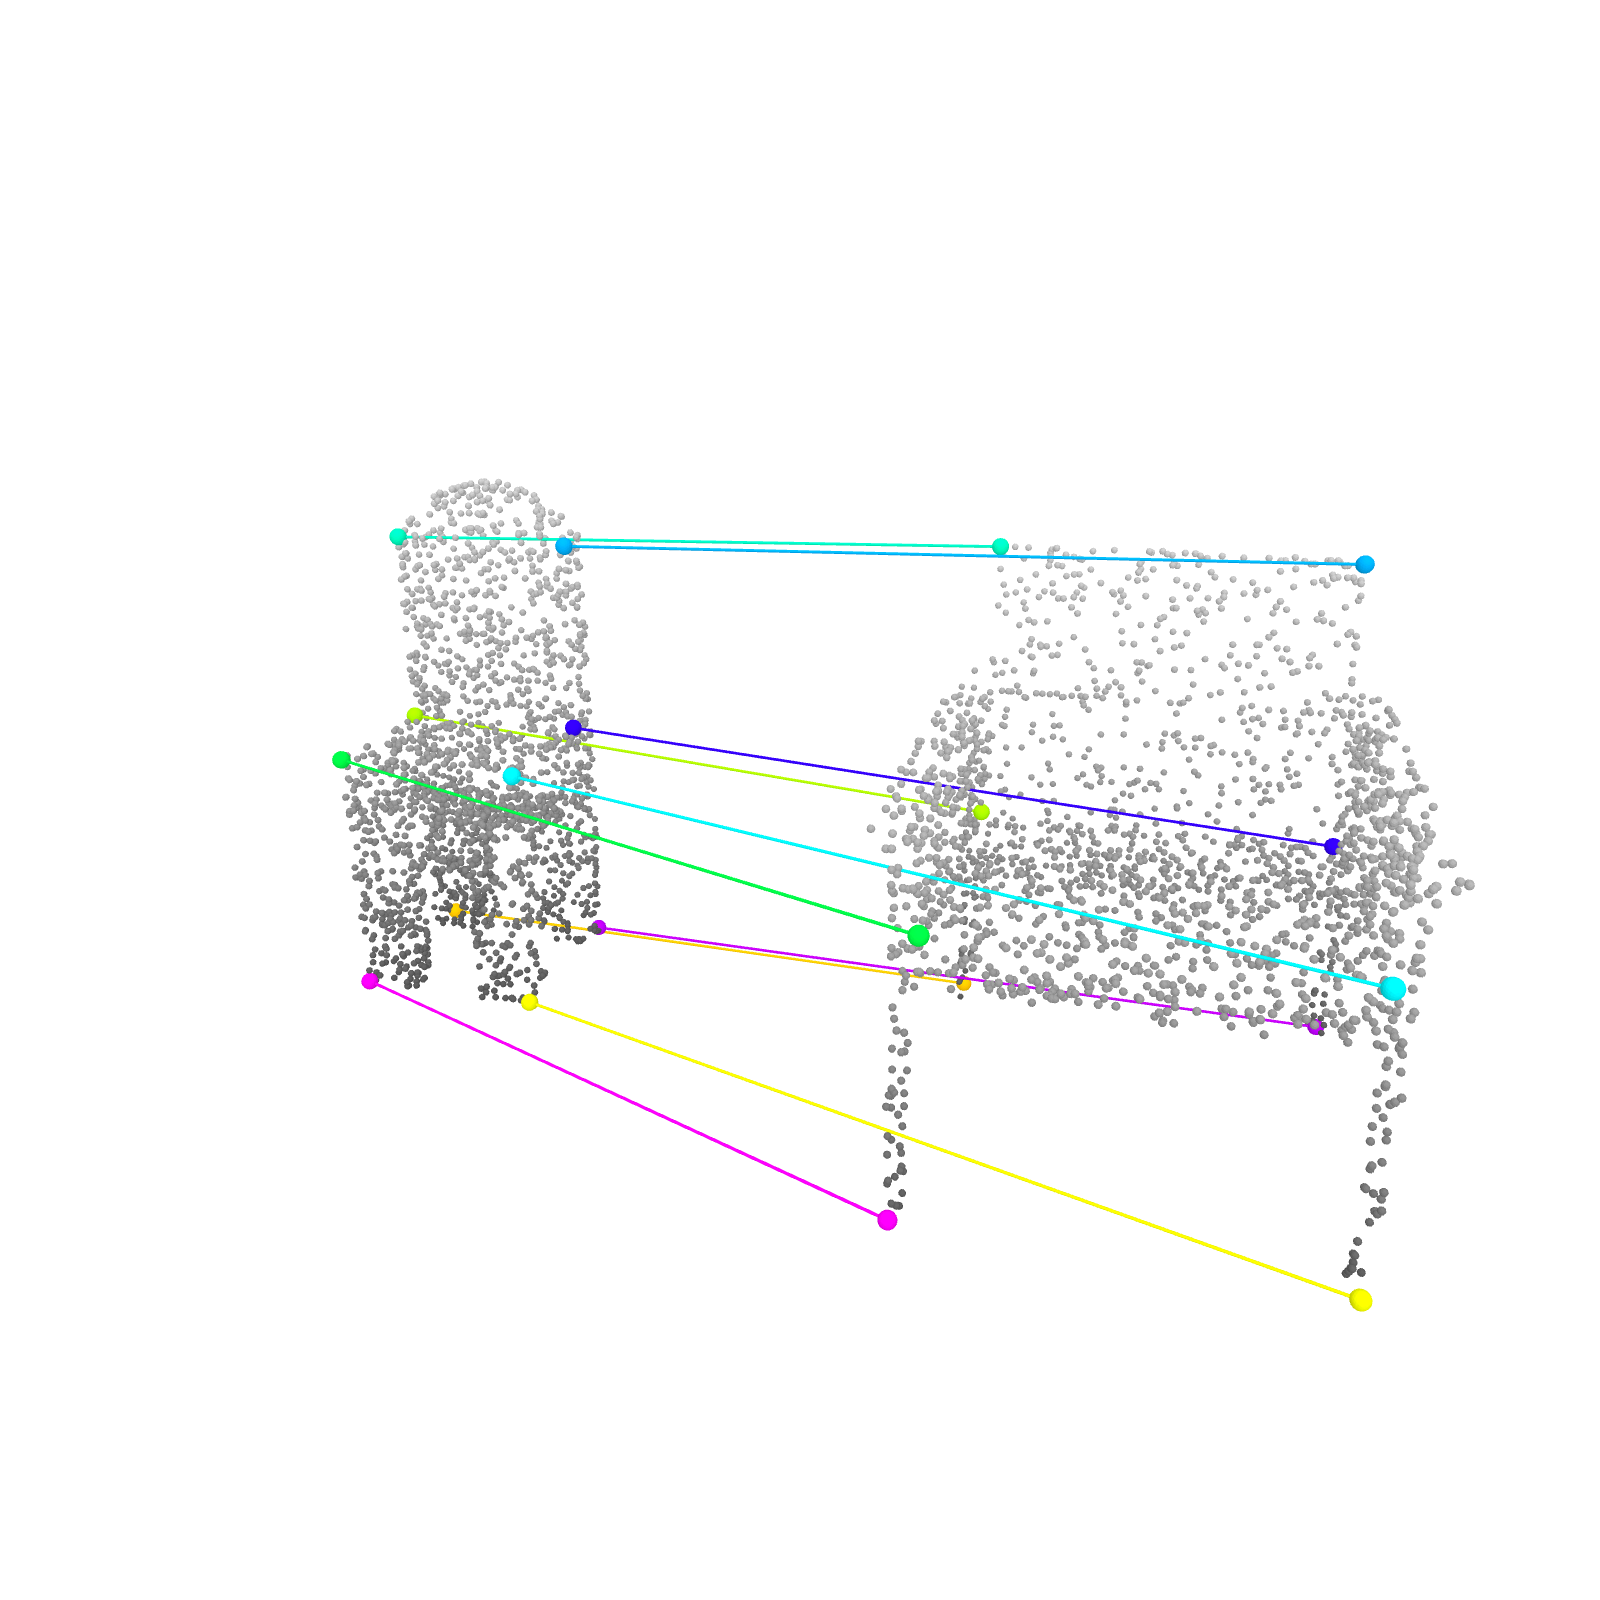
\includegraphics[trim={10 150 10 400},clip,width=\linewidth,height=\linewidth,keepaspectratio]{sup_mat/figures/chair_top11_2828b98d_x_4647b2b9_yaw-164p94_pitch69p52.png}
        \caption{Chair}
        \label{fig:square_chair}
    \end{subfigure}

    \begin{subfigure}[b]{0.45\linewidth}
        \centering
        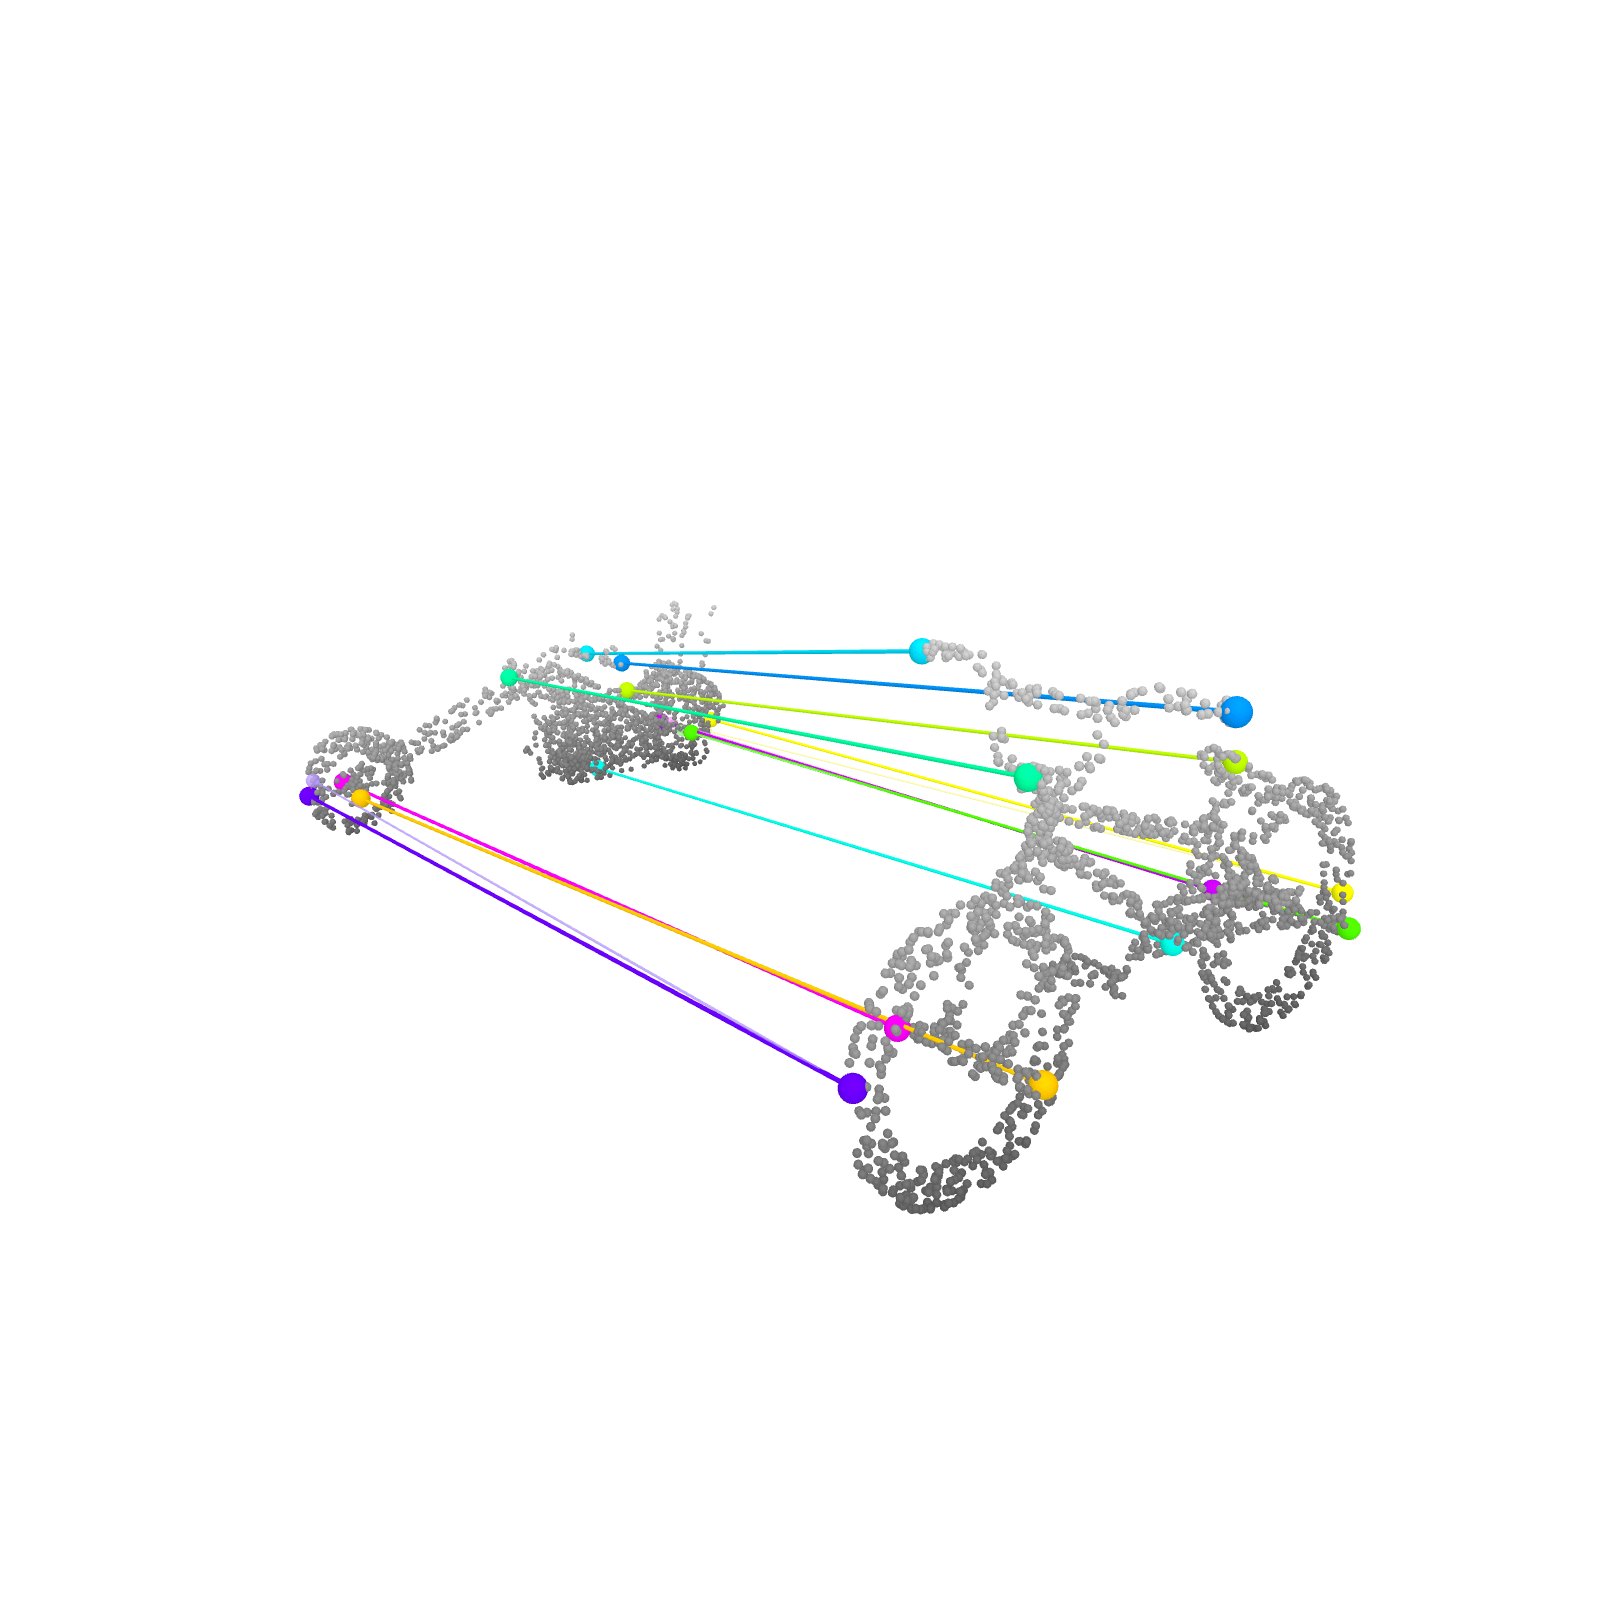
\includegraphics[trim={10 350 10 400},clip,width=\linewidth,height=\linewidth,keepaspectratio]{sup_mat/figures/motorcycle_top03_1d8fb258_x_a1553e0b_yaw-131p95_pitch72p26.png}
        \caption{Motorcycle}
        \label{fig:square_motorcycle}
    \end{subfigure}
    \begin{subfigure}[b]{0.45\linewidth}
        \centering
        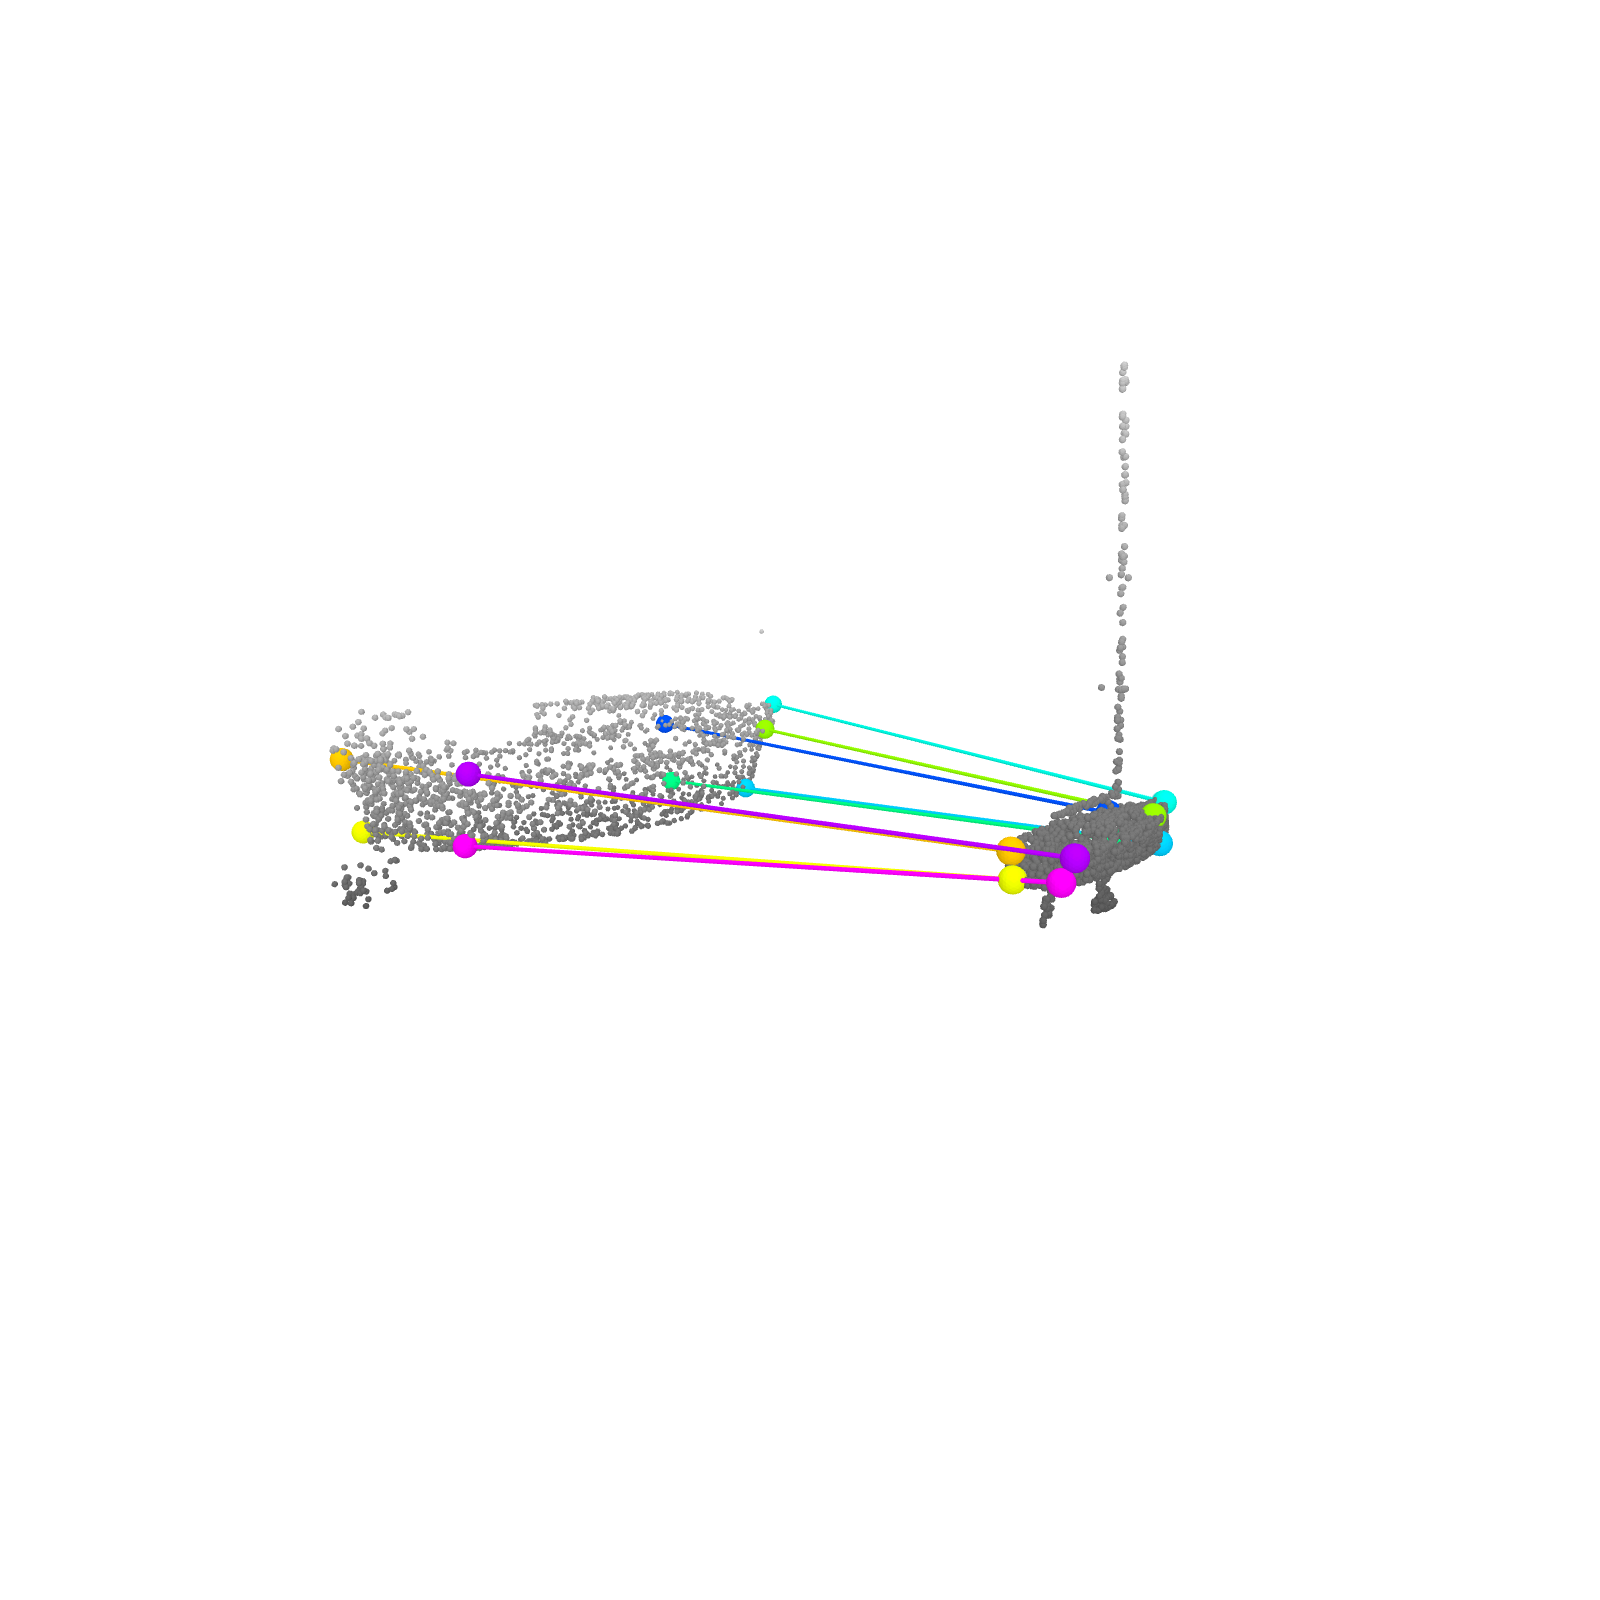
\includegraphics[trim={10 550 10 400},clip,width=\linewidth,height=\linewidth,keepaspectratio]{sup_mat/figures/vessel_top02_cc6656ba_x_e604463b_yaw-325p50_pitch80p49.png}
        \caption{Vessel}
        \label{fig:square_vessel}
    \end{subfigure}

    \caption{\textbf{KeypointNet \cite{you2020} examples with strong annotation agreement.}
    Predicted correspondences are shown in lighter colors, while human annotations are shown in darker colors. The strong overlap between the two indicates that our pipeline recovers correspondences that are highly consistent with human semantic annotations.}
    \label{fig:keypointnet_strong_overlap}
\end{figure}









\clearpage
\section{Additional Quantitative Results on SPair-71k}
\label{sup:supp_spair}

We provide additional evaluation results on SPair-71k \cite{min2019spair71k} across multiple PCK thresholds and training regimes. While the main paper reports PCK@0.10 (see \autoref{tab:spair_pck010}), here we analyze performance at stricter and looser thresholds, and compare four training strategies: \emph{Synth-only}, \emph{Both} (joint real and synthetic training), \emph{Real-only}, and \emph{Synth$\rightarrow$Real} (pretraining on synthetic correspondences followed by fine-tuning on real data).

\paragraph{MARCO \cite{cuttano2026marco} results.}
Across all thresholds (PCK@0.01-0.20), the Synth$\rightarrow$Real setting consistently outperforms Real-only training at practical thresholds. In particular, improvements of $+2.4$ to $+2.9$ PCK are observed for PCK@0.05--0.20. At PCK@0.10, performance improves from $86.39$ to $89.28$, matching the results reported in \autoref{tab:spair_pck010}.

At very strict thresholds (PCK@0.01), Synth$\rightarrow$Real slightly underperforms Real-only ($-2.17$). However, this gap disappears at more relaxed thresholds, where Synth$\rightarrow$Real consistently achieves the best performance.

We also observe that joint training (\emph{Both}) underperforms Real-only, indicating that naive mixing of synthetic and real data is suboptimal, and that a two-stage training strategy is more effective.

\paragraph{GeoAware-SC \cite{zhang2024tellingLeftFromRight} results.}
We observe the same qualitative trend for GeoAware-SC. Synth$\rightarrow$Real consistently improves over Real-only training across all evaluated thresholds, while Synth-only performs poorly in isolation. Joint training again underperforms Real-only, reinforcing that synthetic correspondences are most effective as a pretraining signal rather than as direct supervision.

At PCK@0.10, as we see in the results from the main paper (\autoref{tab:spair_pck010}), synthetic pretraining improves performance from $79.36$ to $83.73$, corresponding to a gain of $+4.37$ PCK.

\paragraph{Cross-architecture consistency.}
Using the PCK@0.10 results from \autoref{tab:spair_pck010}, we observe consistent improvements across architectures and feature choices:
\begin{center}
\begin{tabular}{lccccc}
\toprule
Architecture & DINOv2 \cite{oquab2024dinov2} & Stable Diffusion \cite{rombach2022stablediffusion} & Real-only & Synth$\rightarrow$Real & Gain \\
\midrule
GeoAware-SC \cite{zhang2024tellingLeftFromRight} & \checkmark & \checkmark & 79.36 & 83.73 & +4.37 \\
MARCO \cite{cuttano2026marco}      & \checkmark & $\times$ & 86.39 & 89.28 & +2.89 \\
\bottomrule
\end{tabular}
\end{center}

GeoAware-SC \cite{zhang2024tellingLeftFromRight} uses both DINOv2 \cite{oquab2024dinov2} and Stable Diffusion \cite{rombach2022stablediffusion} features, while MARCO \cite{cuttano2026marco} relies on DINOv2 features without Stable Diffusion. The gains across both settings suggest that our synthetic pretraining signal is not tied to a specific feature family, but provides useful semantic-geometric supervision across different recent correspondence models.

These consistent gains suggest that the benefit of synthetic pretraining is largely architecture-agnostic. Rather than improving a specific model design, the generated correspondences provide a strong pretraining signal that improves representation quality across different backbones and matching heads.

\paragraph{Summary.}
Overall, these results support three key observations: (i) synthetic correspondences alone are insufficient for high performance, (ii) naive joint training is suboptimal, and (iii) a two-stage Synth$\rightarrow$Real strategy consistently yields the best results. This pattern holds across architectures and evaluation thresholds, reinforcing the generality of the proposed data generation pipeline.

% Add your qualitative figures / tables here
% Example:
% \subimport{./sup_mat/figures}{qualitative_results}
% \subimport{./sup_mat/figures}{more_spair_vis}
% \subimport{./sup_mat/figures}{more_keypointnet_vis}
\clearpage
\section{Extended Ablation Study}
\label{sup:ablation_study}
\subsection{Registration Method Ablation}
\label{sup:ablation_registration}

We ablate the deformation model used in the registration stage prior to correspondence extraction. All other components are kept fixed, including lifted DINOv2 \cite{oquab2024dinov2} features, nearest-neighbor assignment, and the semantic threshold $\tau_{\mathrm{sem}}=0.85$. We compare our default continuous piecewise-affine (CPA) model with two alternatives: a global affine transformation and a thin-plate spline (TPS) deformation.

\paragraph{Affine.}
As a global transformation baseline, we use an affine transformation

\[
f(\mathbf{x}) = \mathbf{A}\mathbf{x} + \mathbf{t},
\]
where $\mathbf{A} \in \mathbb{R}^{3\times 3}$ and $\mathbf{t} \in \mathbb{R}^{3}$. This model has 12 learnable parameters and is optimized with Adam using the same Chamfer objective. Since it cannot model non-rigid variation, it serves as a baseline for how much alignment can be explained by global pose normalization alone.

\paragraph{Continuous Piecewise-Affine (CPA).}
Our default model uses a $6 \times 6 \times 6$ control grid (216 vertices) over the normalized 3D domain, tetrahedralized via Delaunay triangulation. Each vertex has a learnable displacement, and each point is warped using barycentric interpolation within its enclosing tetrahedron. This yields a deformation that is locally affine and globally continuous. We enforce smoothness by penalizing squared differences between neighboring vertex displacements, with $\lambda_{\mathrm{smooth}}=0.3$. The model has 648 degrees of freedom.

\paragraph{Thin-Plate Spline (TPS).}
We compare with a classical smooth non-rigid deformation
\[
f(\mathbf{x}) = \mathbf{a} + \mathbf{B}\mathbf{x}
+ \sum_{k=1}^{K} \mathbf{w}_k \, U(\|\mathbf{x}-\mathbf{c}_k\|),
\qquad U(r) = -r,
\]
where $\mathbf{B}\in\mathbb{R}^{3\times3}$, $\mathbf{a}\in\mathbb{R}^{3}$, and $\mathbf{w}_k\in\mathbb{R}^{3}$. We use $K=216$ control points sampled from the source, resulting in a similar number of parameters to CPA (660 vs.\ 648). Smoothness is enforced with an $\ell_2$ penalty on the radial weights.

\paragraph{Protocol.}
We evaluate all three methods on the 16 KeypointNet \cite{you2020} categories. For each category, we sample 100 source-target pairs from random instances and run all methods on them. All hyperparameters are shared: 10,000 Adam iterations with early stopping on a loss plateau, a learning rate of $0.005$, and no pair-level filtering. Performance is measured using PCK at multiple thresholds, where a prediction is correct if it falls within $\tau \cdot d$ of the ground-truth target keypoint, with $d$ the target bounding-box diagonal.

\paragraph{Results.}
\autoref{tab:ablation_registration} reports mean PCK across all categories. CPA achieves the best average performance at four of the five PCK thresholds, while TPS is slightly better only at PCK@0.05. Overall, CPA and TPS obtain very similar accuracy, indicating that the choice of non-rigid basis has limited impact on correspondence quality.

\begin{table}[h!]
\centering
\small
\caption{\textbf{Registration ablation on KeypointNet.}
Mean PCK across all 16 categories. PCK thresholds define the allowed normalized distance from the ground-truth keypoint, measured as a fraction of the target bounding-box diagonal. DOF denotes the number of learnable parameters. Time reports the mean registration time per pair on a single A6000 GPU. Best results are shown in \textbf{bold}.}
\label{tab:ablation_registration}
\setlength{\tabcolsep}{4pt}
\begin{tabular}{lccccccc}
\toprule
Method & DOF & Time (s/pair) & PCK@0.01 & PCK@0.05 & PCK@0.10 & PCK@0.15 & PCK@0.20 \\
\midrule
Affine            & 12  & 1.15 & 0.221 & 0.686 & 0.898 & 0.960 & 0.982 \\
TPS ($K\!=\!216$) & 660 & 3.71 & 0.226 & \textbf{0.739} & 0.919 & 0.966 & 0.983 \\
CPA (ours)        & 648 & \textbf{1.13} & \textbf{0.236} & 0.729 & \textbf{0.922} & \textbf{0.971} & \textbf{0.986} \\
\bottomrule
\end{tabular}
\end{table}

In contrast, CPA is substantially more efficient. It is about $3.3\times$ faster per pair (1.13s vs.\ 3.71s), despite having a similar number of parameters. We also observe that CPA typically converges earlier. This difference arises from the underlying structure: CPA uses local barycentric interpolation within tetrahedra, while TPS requires dense kernel interactions between all points and control points at each iteration.

Compared with the affine baseline, CPA provides clear gains, especially at tighter PCK thresholds, highlighting the importance of non-rigid alignment for cross-instance correspondence.

\paragraph{Conclusion.}
This ablation supports two conclusions: (i) non-rigid deformation is essential for accurate alignment, as affine transformations perform significantly worse; and (ii) among non-rigid models, CPA offers a better accuracy-efficiency tradeoff, achieving similar performance to TPS while being significantly faster and more stable in practice.

\subsection{Ablation on Semantic Filtering}
\label{sup:ablation_semantic_filtering}

We analyze the role of semantic filtering in our pipeline. Specifically, we study (i) the effect of removing semantic filtering entirely, (ii) the contribution of correspondence-level filtering alone, and (iii) the impact of the correspondence-level semantic threshold $\tau_{\mathrm{sem}}$ when combined with pair-level filtering. All experiments are conducted on KeypointNet using the same evaluation protocol as in the main paper.

\subsubsection{No Semantic Filtering}
\label{sup:no_semantic_filtering}

We first evaluate the pipeline without any semantic filtering. In this setting, all object pairs are retained, and correspondences are obtained directly from CPA registration followed by nearest-neighbor assignment.

\autoref{tab:unfiltered} shows that this setting produces significantly lower accuracy. While geometric alignment alone can recover many plausible correspondences, it frequently matches inconsistent regions across instances, leading to degraded PCK, especially at stricter thresholds (e.g., PCK@0.05 and PCK@0.10). This highlights the limitation of relying solely on geometry for cross-instance correspondence and the need for a semantic pruning step.

\subimport{./sup_mat/tables}{unfiltered_keypointnet}

\subsubsection{Correspondence-Level Semantic Filtering Only}
\label{sup:only_corr_filtering}

We next evaluate correspondence-level semantic filtering alone, without pair-level filtering. In this setting, all object pairs are retained, and individual correspondences are pruned using a fixed threshold $\tau_{\mathrm{sem}}=0.85$.

\autoref{tab:pck_results} shows that this step alone leads to a substantial improvement over the no-filtering baseline. In particular, mean PCK@0.10 improves from 0.84 to 0.91, confirming that a large portion of the error arises from semantically inconsistent matches that are geometrically plausible but incorrect.

\subimport{./sup_mat/tables}{only_sem_fil_table}

\subsubsection{Correspondence-Level Semantic Threshold}
\label{sup:ablation_semantic_threshold_corr}

We finally analyze the effect of the semantic threshold $\tau_{\mathrm{sem}}$ when combined with pair-level filtering, as used in the full pipeline.

This threshold controls an accuracy-coverage tradeoff. A stricter threshold keeps fewer but more reliable matches, while a looser threshold retains more matches but allows more semantically inconsistent correspondences. To quantify coverage, we report the \emph{median GT-used rate} across categories. A ground-truth keypoint is counted as used if at least one surviving correspondence remains within $0.05$ of the object bounding-box diagonal from the ground-truth location.

Importantly, this metric is conservative. KeypointNet annotations are sparse and typically located on salient corners or extreme parts, while our method produces dense correspondences across the object surface (see Fig.~1). As a result, semantically valid correspondences that do not fall within the $0.05$ evaluation radius are still counted as missed.

\begin{table}[h!]
\centering
\small
\caption{\textbf{Ablation on the correspondence-level semantic threshold (with pair-level filtering).}
Results are averaged over three random seeds and 16 KeypointNet categories. Median GT-used rate denotes the median fraction across categories of ground-truth keypoints that remain evaluable after correspondence-level pruning.}
\label{tab:semantic_threshold_ablation}
\setlength{\tabcolsep}{5pt}
\begin{tabular}{lccccc}
\toprule
$\tau_{\mathrm{sem}}$ & PCK@0.05 $\uparrow$ & PCK@0.10 $\uparrow$ & PCK@0.15 $\uparrow$ & PCK@0.20 $\uparrow$ & Median GT-used rate $\uparrow$ \\
\midrule
0.50 & 0.758 & 0.930 & 0.974 & 0.988 & 0.260 \\
0.85 & 0.749 & 0.926 & 0.973 & 0.989 & 0.576 \\
1.50 & 0.699 & 0.896 & 0.960 & 0.983 & 0.915 \\
\bottomrule
\end{tabular}
\end{table}

\autoref{tab:semantic_threshold_ablation} shows that the choice of threshold controls a clear tradeoff between accuracy and coverage. A strict threshold ($\tau_{\mathrm{sem}}=0.5$) achieves the highest accuracy but retains only 26.0\% of ground-truth keypoints, while a loose threshold ($\tau_{\mathrm{sem}}=1.5$) retains 91.5\% but significantly degrades accuracy.

We therefore use $\tau_{\mathrm{sem}}=0.85$ as a practical middle point: it maintains similar accuracy to the stricter threshold while more than doubling the median GT-used rate (26.0\% $\rightarrow$ 57.6\%).

\paragraph{Discussion.}
Overall, these results show that semantic filtering is essential for removing geometrically plausible but semantically incorrect correspondences. Most of the improvement comes from correspondence-level filtering, while pair-level filtering provides an additional refinement by removing object pairs with insufficient semantic overlap.

\clearpage
\section{Qualitative Analysis of DINOv2 Based Semantic Filtering}
\label{sup:supp_semantic_analy}

We provide a qualitative analysis of the DINOv2 based semantic filtering used in our pipeline, both at the pair level and at the correspondence level. As shown in \autoref{fig:semantic_coverage_analysis}, we visualize the lifted DINOv2 features after joint PCA to three dimensions, and mark points according to whether they have any sufficiently similar semantic counterpart in the paired object. Green points have at least one point in the paired object with cosine similarity above our threshold of \(0.85\), while red points have no such candidate. We use this semantic coverage to filter object pairs that do not share enough semantic structure. In addition, for pairs that survive pair-level filtering, red points are guaranteed to be removed by our semantic pruning after registration. This filtering is complementary to the correspondence-level pruning, which further removes geometrically matched points whose assigned matches are semantically inconsistent.

\begin{figure}[h]
    \centering
    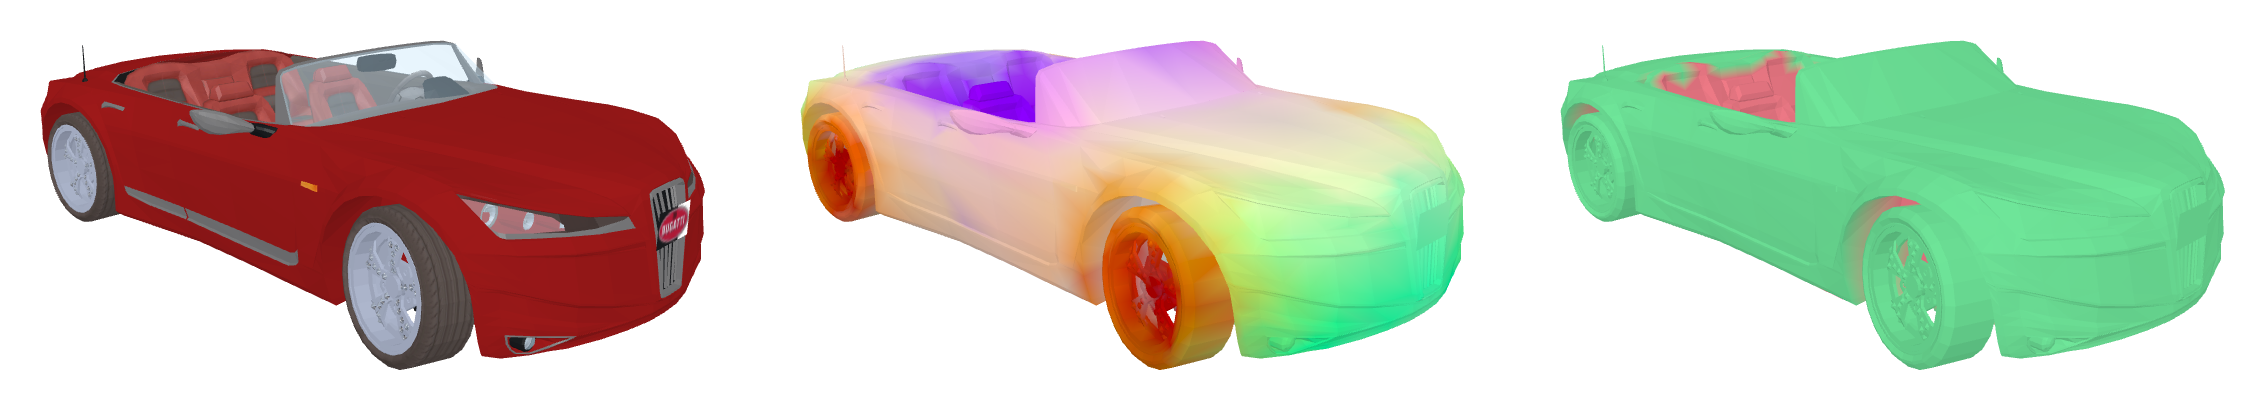
\includegraphics[width=\linewidth]{figures/semantic_analysis/src_triplet_view1.png}\\[-1mm]
    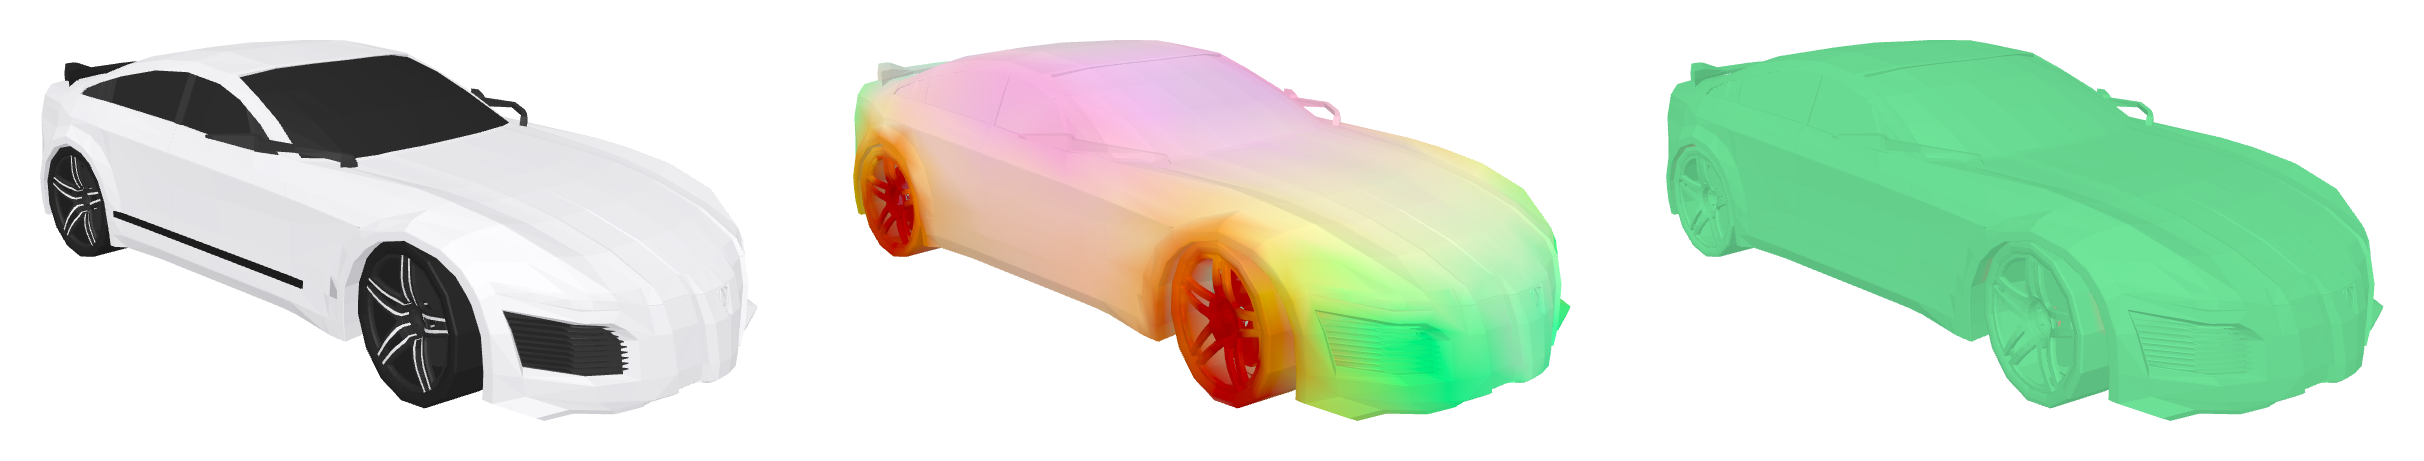
\includegraphics[width=\linewidth]{figures/semantic_analysis/tgt_triplet_view1.png}\\[1mm]
    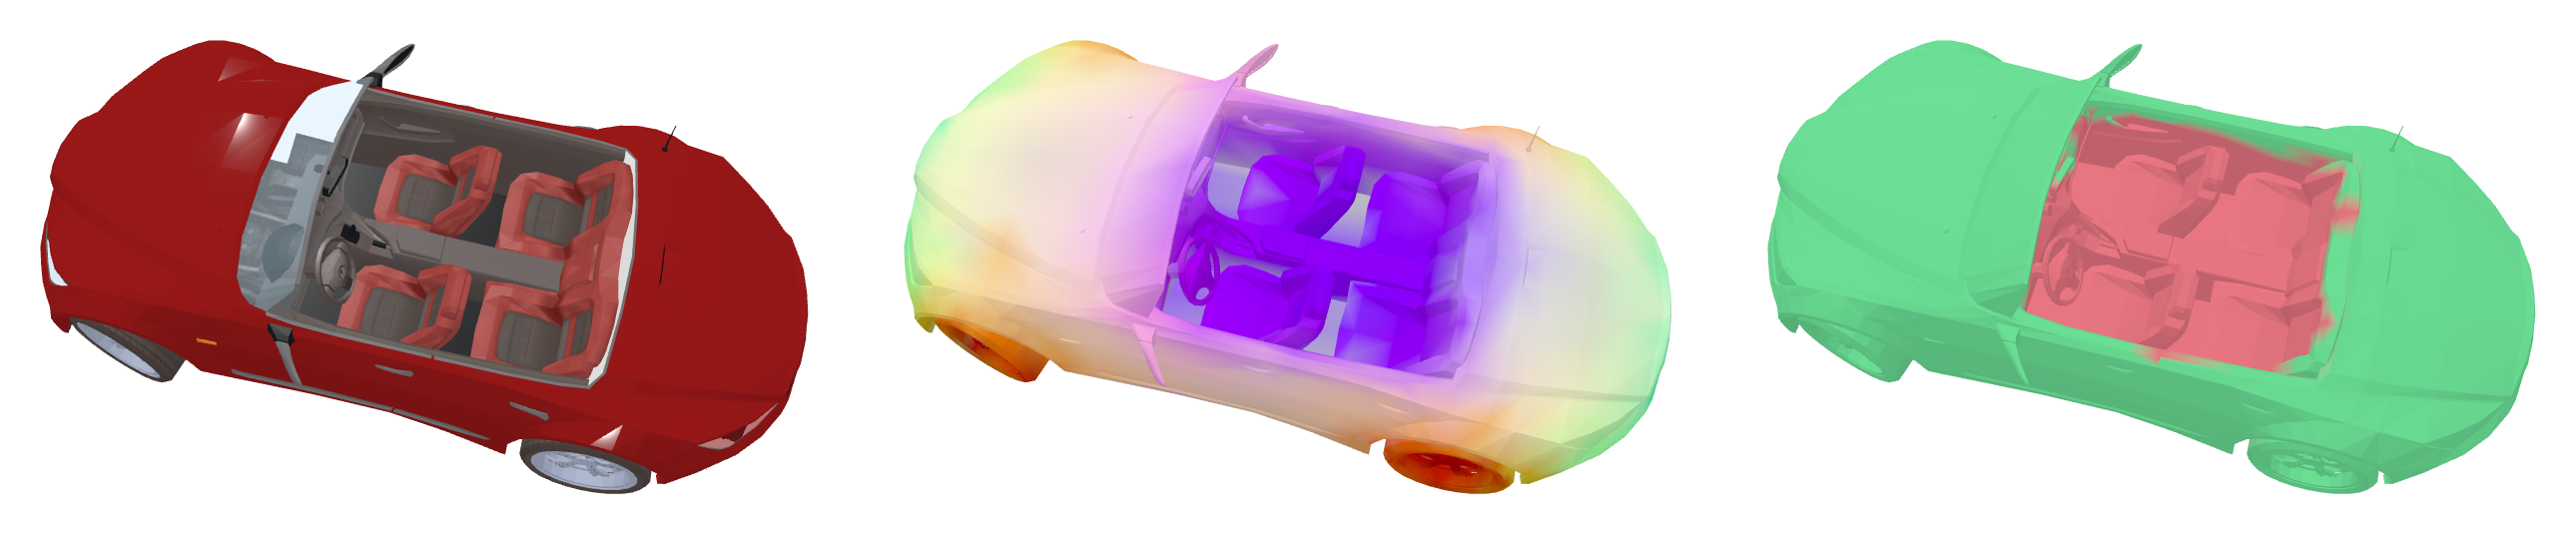
\includegraphics[width=\linewidth]{figures/semantic_analysis/src_triplet_view2.png}\\[-1mm]
    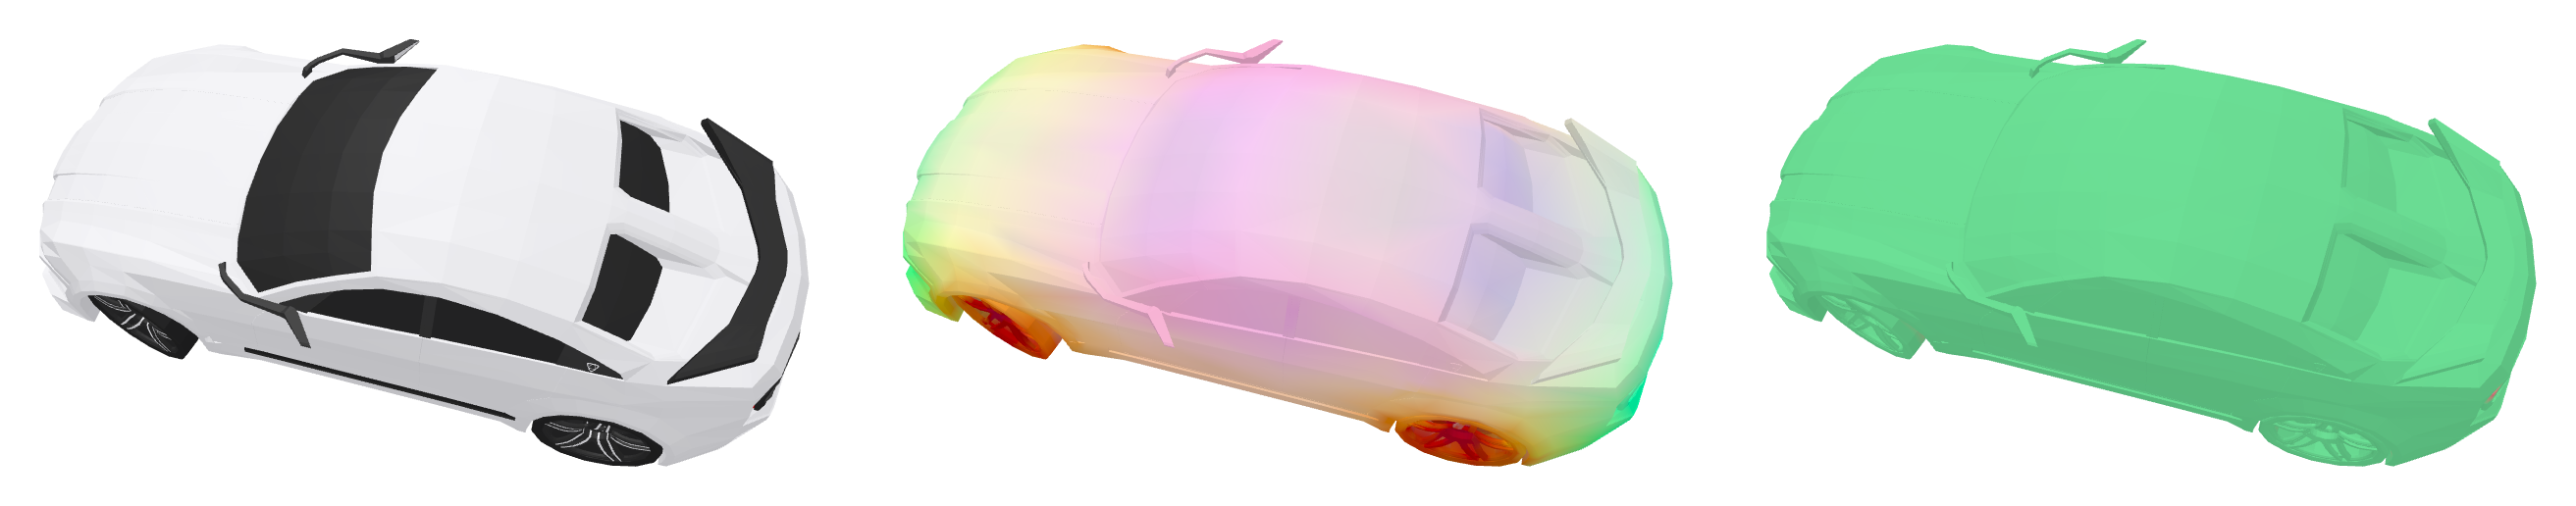
\includegraphics[width=\linewidth]{figures/semantic_analysis/tgt_triplet_view2.png}
\caption{
Qualitative analysis of DINOv2 based semantic coverage. Each row shows the original rendering, a PCA visualization of DINOv2 features computed jointly for the object pair, and the resulting semantic coverage mask. Green points have at least one semantically similar point in the paired object, while red points have none.
}
    
    \label{fig:semantic_coverage_analysis}
\end{figure}


We further visualize sampled correspondences established by our method in \autoref{fig:semantic_correspondence_pruning}. For visualization, we sample farthest points from the final correspondence set after semantic pruning. Each row shows a different view of the same object pair. As can be seen, semantically unmatched regions such as the exposed seats and steering wheel of the roofless car do not obtain correspondences. Similarly, the roof region of the white car is also removed, even though the CPA registration geometrically deforms these regions toward other object parts. These correspondences are filtered by our semantic correspondence pruning stage due to semantic inconsistency.
\clearpage
\begin{figure}[t]
    \centering
    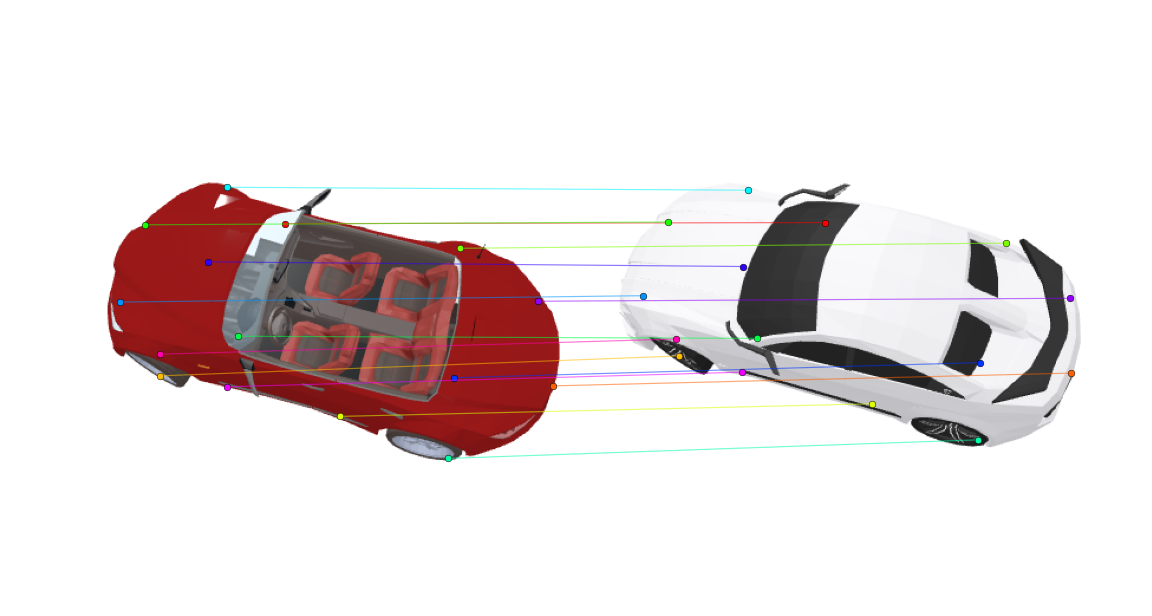
\includegraphics[
        width=0.9\linewidth,
        height=0.26\textheight,
        keepaspectratio,
        trim={20pt 80pt 20pt 80pt},
        clip
    ]{figures/semantic_analysis/sparse15_view10.png}\\[-2mm]
    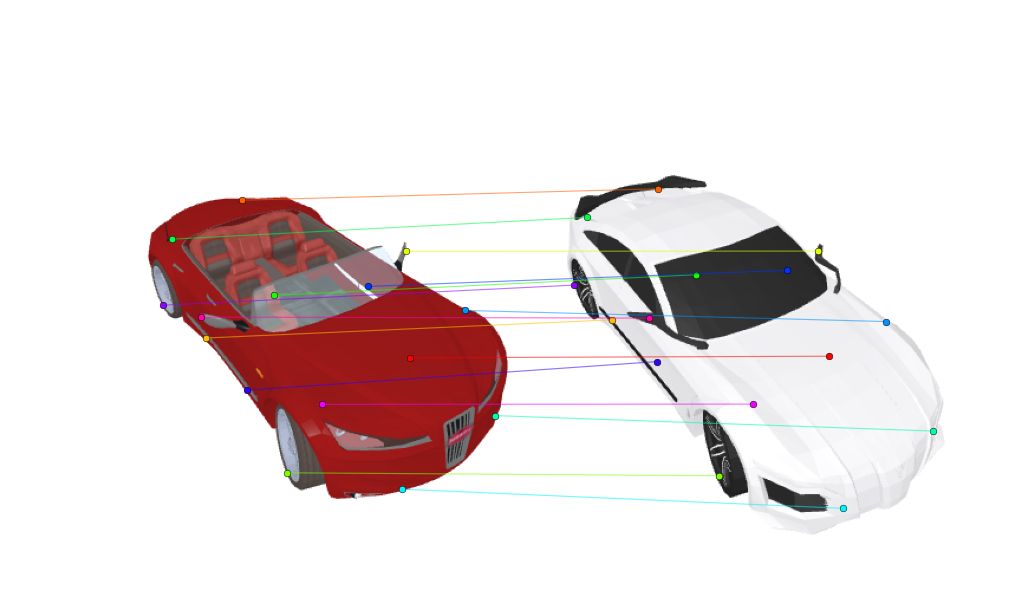
\includegraphics[
        width=0.9\linewidth,
        height=0.26\textheight,
        keepaspectratio,
        trim={20pt 50pt 20pt 80pt},
        clip
    ]{figures/semantic_analysis/sparse15_view34.png}
    \caption{
    Sampled correspondences after semantic pruning. Each row shows a different view of the same object pair.
    }
    \label{fig:semantic_correspondence_pruning}
\end{figure}

\section{Detailed PCK Results by Semantic Label and KeypointNet Category}
\label{Sup:per_label}

We provide a detailed analysis of correspondence quality at the level of individual semantic keypoints. For each category, we evaluate up to 100 objects and all induced source-target pairs, corresponding to up to $\binom{100}{2}$ object pairs per category, across 16 categories and 79,200 pairs overall. We report PCK results per annotated semantic label, following the KeypointNet \cite{you2020} evaluation protocol.

These results are computed using our full pipeline, including correspondence-level semantic filtering with $\tau_{\mathrm{sem}}=0.85$ and pair-level filtering. For each semantic label, we report results as $\text{correct}/\text{total}$, where \emph{total} denotes the number of ground-truth keypoints that remain evaluable after filtering. A keypoint is considered evaluable if at least one predicted correspondence remains within $0.05$ of the object bounding-box diagonal from the ground-truth location. We report raw $\text{correct}/\text{total}$ counts rather than percentages to make the amount of retained evaluable annotations explicit for each semantic label.

KeypointNet annotations are sparse and typically located on salient corners or extreme parts, while our method produces dense correspondences across the object surface. Therefore, these per-label results should be interpreted as a conservative estimate of correspondence quality around the sparse annotated locations.

The full per-label results are reported in 
Tables~\ref{tab:pck_airplane}-\ref{tab:pck_vessel}.


\subimport{./sup_mat/tables}{labels_airplane}

%shira added
\clearpage
\subimport{./sup_mat/tables}{semantic_thresh_values_tables}

% \clearpage
% \subimport{./sup_mat/figures}{keypointnet_fig}
% \subimport{./sup_mat/figures}{failure_cases_keypointnet}

\begin{comment}
        \item[\autoref{Sup:MoreExpRes}.] Additional experiments and results:
            \begin{enumerate}[label=\arabic*)] 
                \item Comparisons on $N=3$ cases (\autoref{fig:triplets})
                \item Camera overlap expressiveness  (\autoref{Fig:5cam}).
                \item Fast Moving Videos from  StabStitch-D dataset ~\cite{Nie:ECCV:2024:stabstitch} (\autoref{fig:fm})
            \end{enumerate}
         \refstepcounter{enumi}   
        \item [\autoref{Sup:ArchN=3}.] An example MVS architecture Plot for an $N>2$ case (\autoref{Fig:method})
        \refstepcounter{enumi}
        \item[\autoref{sec:geovar}.] The Geometric Variance metric
        \refstepcounter{enumi}
        \item[\autoref{sec:arch}.] Additional architecture details: AE and the Alignment Network
\setcounter{figure}{4}
\setcounter{table}{3}      % 4 + 1 → 5
\clearpage

\section{Additional Experiments and Results}\label{Sup:MoreExpRes}
\subimport{./supp_mat/}{experiments_and_results}

\clearpage


\section{An Example for the MVS Architecture for an $N>2$ Case}\label{Sup:ArchN=3}
In the paper, due to page
limit, we show a visualization of 
our MVS architecture
for the case of $N=2$. 
The case of $N>2$ is handled
similarly: in the prepossessing the DINO, PCA and AE steps are still done per cameras,
while the ORT extraction
is still done in a pairwise
fashion. 
Stage 1, based on the geometric loss, utilized 
all the relevant pairs. 
Similarly, this is also the case in Stage 2, where,
for every $t$, 
there are now 3 pairs 
for each time step $t$,
along with three temporal pairs (for $t$ and $t+1$
in each of the $N=3$ cameras).
The architecture,
by design, naturally generalizes
to the case of even 
higher $N$ values. 

\subimport{./supp_mat/}{fig_method} 

\clearpage

\section{The Geometric Variance metric}
\label{sec:geovar}
\subimport{./supp_mat/}{geometric_variance} 
\clearpage

\subimport{./supp_mat/}{arch_details} 


\clearpage
\bibliography{refs}
%\bibliographystyle{abbrvnat}
\bibliographystyle{unsrt}
\end{comment}
% \end{document}